\chapter{RESULTADOS}\label{sec:Resultados}

En este capítulo se exponen los resultados que se han ido obteniendo a lo largo del proyecto. La idea es ir reconstruyendo el camino experimental que llevó a obtener los resultados finales. Se explicará qué ideas se probaron primero, qué problemas surgieron, qué hipótesis aparecieron a partir de los datos y qué cambios fueron mejorando el modelo.

Hay una aclaración importante antes de empezar. El paper de ChemEq25 compara modelos de detección como \textit{YOLOv11} o \textit{RF-DETR} \citebox{hossain2025chemistrylabdataset}. En este TFG el planteamiento final no es detección, sino clasificación de crops generados a partir de las anotaciones YOLO. Por tanto, las métricas como \textit{accuracy}, F1 o \texttt{classification\_mAP} sirven para evaluar nuestro clasificador, pero no son directamente equivalentes al \textit{mAP@50} de un detector. Aun así, sí permiten demostrar que un modelo de \textit{deep learning} basado en TN puede funcionar de forma competitiva en un problema de clasificación de imágenes.

\section{Primeros experimentos con Flowers102}

Flowers102 fue el dataset de prueba inicial. No era el objetivo final del TFG, pero sirvió para comprobar que el pipeline entrenaba, que las métricas se guardaban bien y que la red tensorial recibía gradientes. Además, al tener 102 clases, era un buen primer dataset de prueba para detectar si el modelo estaba aprendiendo algo o si se quedaba cerca del azar.

\subsection{Modelo original CustomTTN}

Con el modelo original \texttt{CustomTTN} se hicieron los primeros experimentos. Los resultados fueron los siguientes:

\begin{figure}[H]
    \centering
    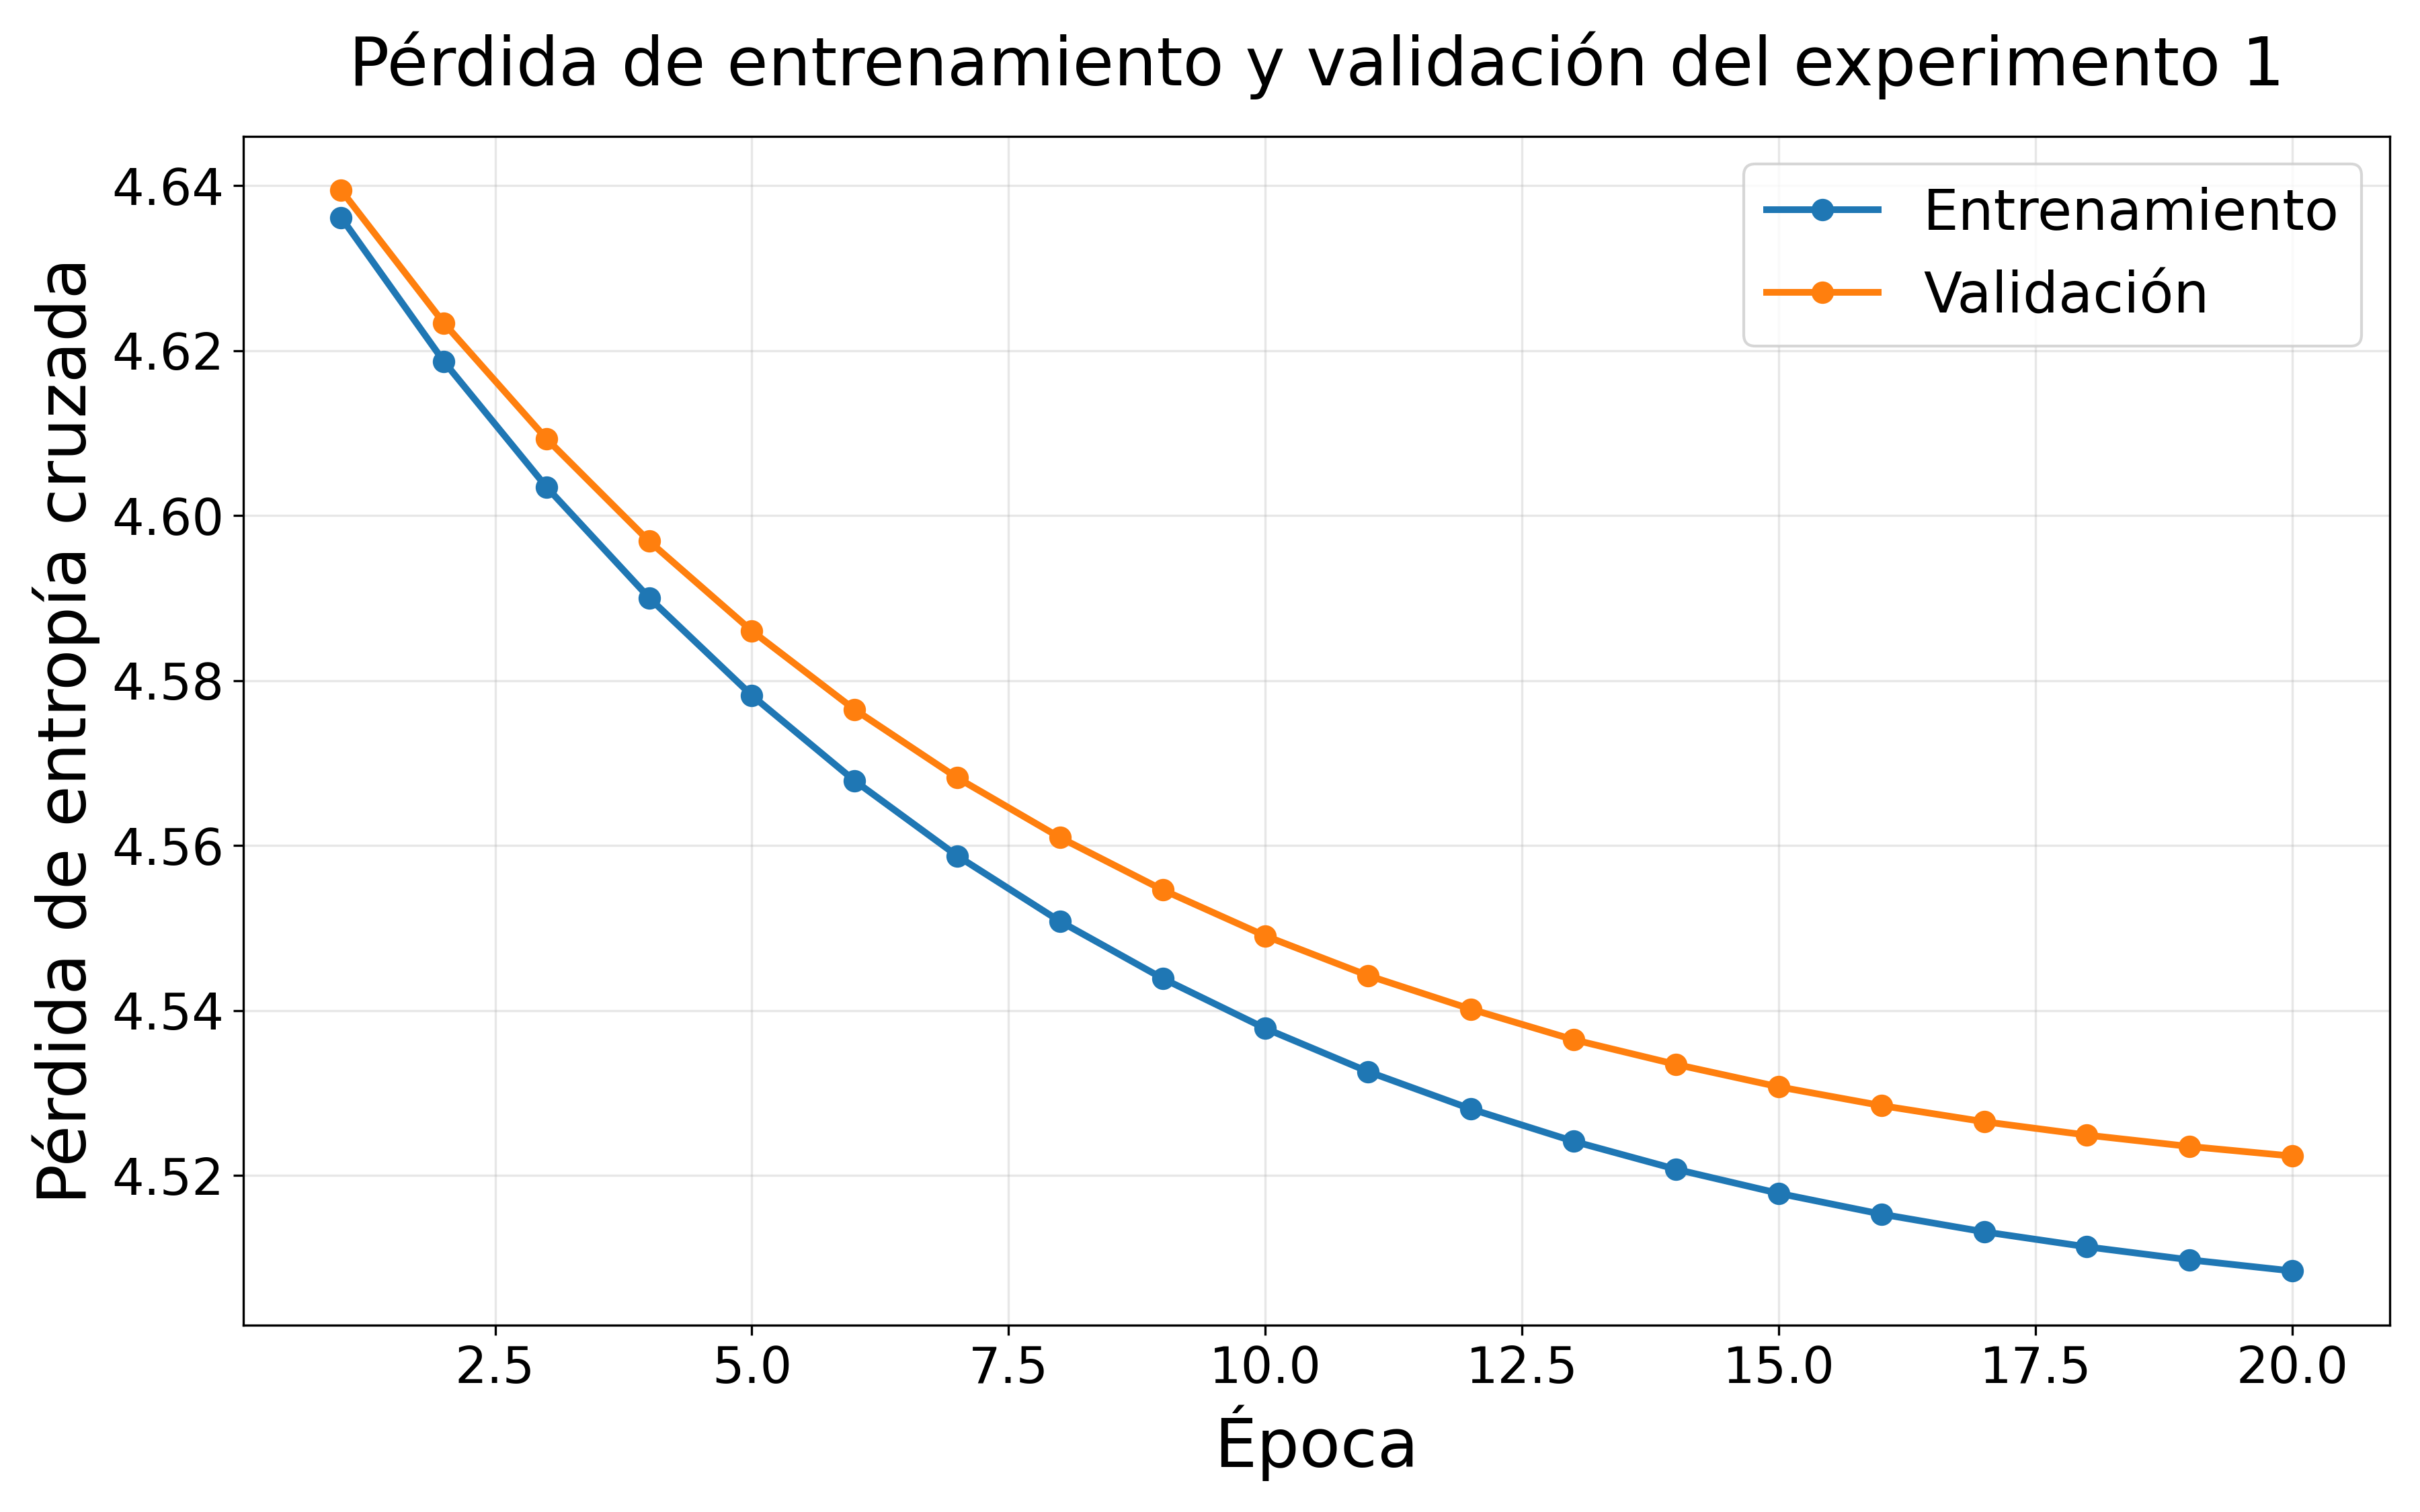
\includegraphics[width=0.55\linewidth]{figures/Experiments_logs/loss_curve_04-21.png}
    \caption{Curvas de pérdida del primer experimento con \texttt{CustomTTN} sobre Flowers102.}
    \label{fig:loss_curve_04-20}
\end{figure}

\begin{table}[H]
\centering
\small
\begin{tabular}{lcccc}
\toprule
\textbf{Experimento} & \textbf{Mejor acc. eval} & \textbf{Época} & \textbf{Mejor eval loss} & \textbf{Eval loss final} \\
\midrule
\texttt{1} & 3,58\% & 9 & 4,5153 & 4,5156 \\
\bottomrule
\end{tabular}
\caption{Resumen representativo del primer experimento con \texttt{CustomTTN}.}
\label{tab:customttn_inicial}
\end{table}

En este momento se estaba usando Flowers102. Si calculamos $\ln(102)$ se obtiene aproximadamente $4,625$, que está muy cerca de la pérdida que aparece en la gráfica. Esto significa que el modelo estaba muy próximo a un comportamiento aleatorio. La \textit{train loss} bajaba muy poco y la precisión de evaluación se quedaba alrededor del 3,6\%. Por tanto, aunque el código ya funcionaba, el modelo todavía no estaba aprendiendo una representación útil.

\subsection{Hipótesis 1}

A raíz de estos resultados se elaboró la primera hipótesis. El modelo no aprendía bien porque entre las contracciones tensoriales no había funciones no lineales como ReLU, sigmoide o SeLU. Esta hipótesis tenía sentido porque, como se vio en el marco teórico, las redes neuronales profundas no se basan solo en aplicar transformaciones lineales, sino en intercalar activaciones no lineales que aumentan su capacidad expresiva.

La idea inicial fue aplicar estas funciones en cada salida resultante de la contracción de cada bloque MPS. Sin embargo, esto no era tan directo en TensorKrowch, porque los nodos resultantes de una contracción no se pueden modificar como si fueran tensores PyTorch normales. Por eso fue necesario cambiar la estructura del modelo y dividir la TTN en niveles independientes.

\subsection{Modelo HybridCustomTTN}

Después de aplicar el cambio de la hipótesis 1, se lanzó un nuevo experimento. El modelo ya no era una TTN monolítica, sino una arquitectura híbrida; cada nivel contraía bloques MPS-3 con TensorKrowch y entre niveles se aplicaban transformaciones PyTorch del tipo \texttt{LayerNorm -> Linear -> ReLU}.

\begin{figure}[H]
    \centering
    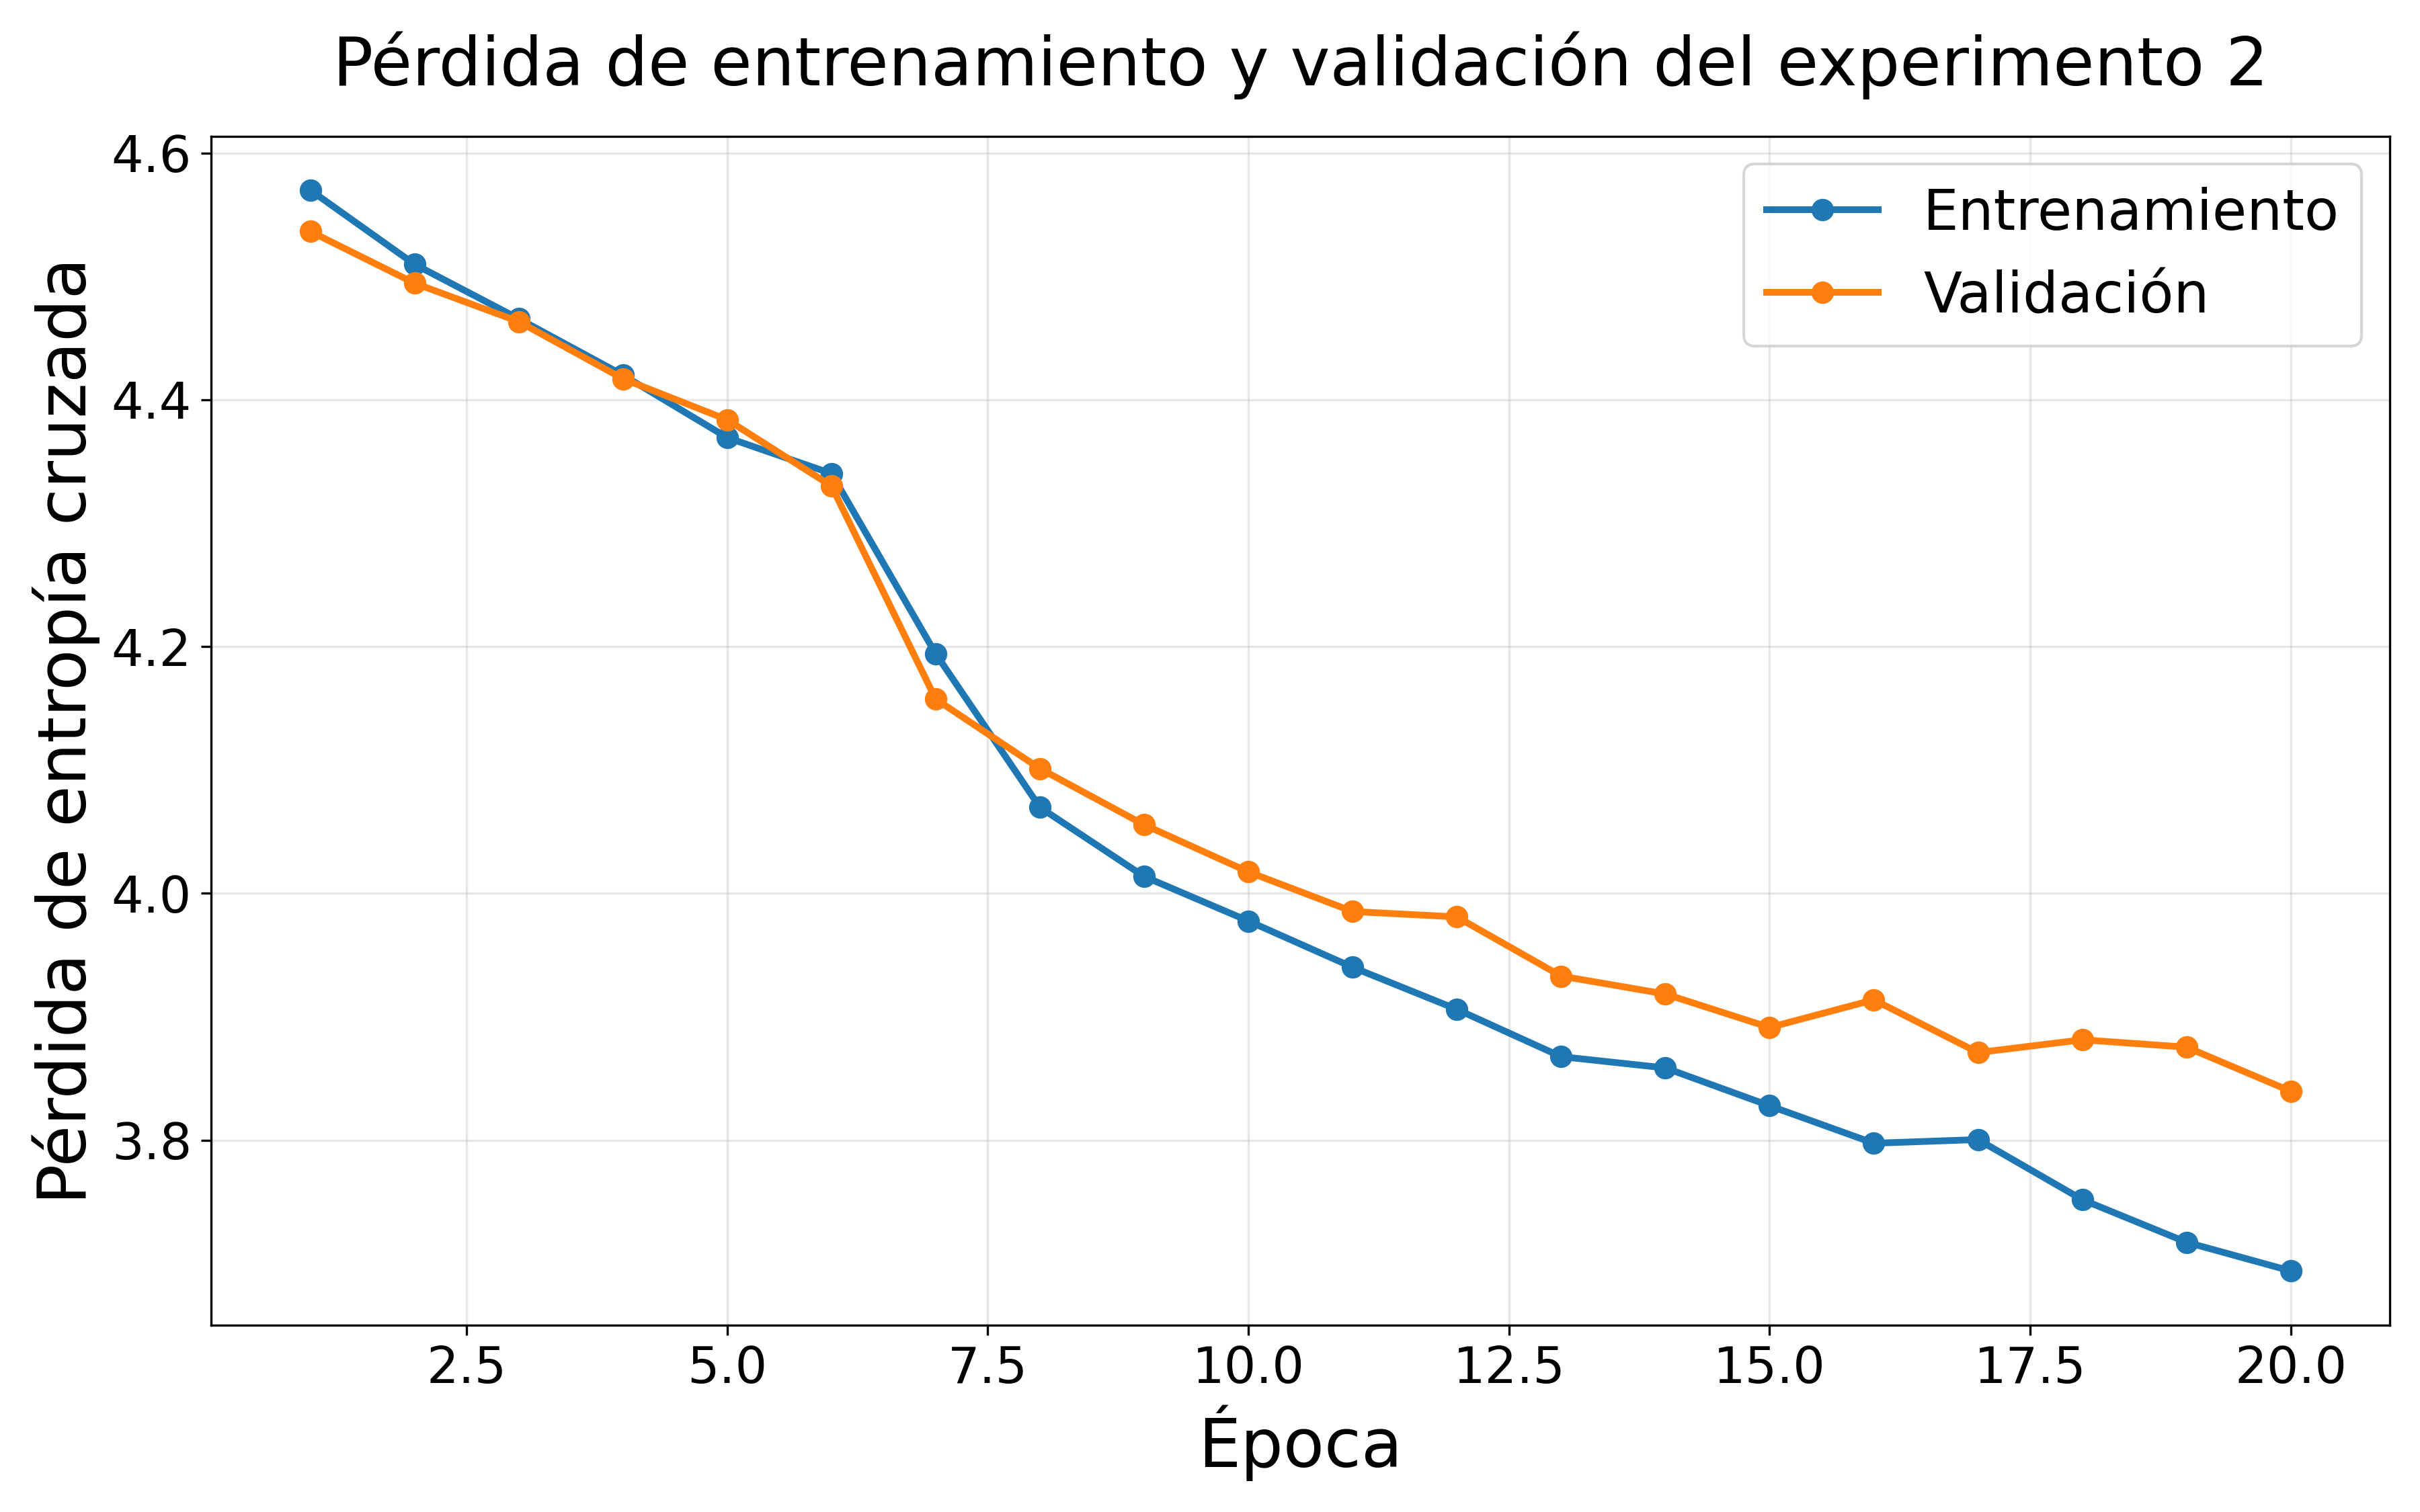
\includegraphics[width=0.55\linewidth]{figures/Experiments_logs/loss_curve_04-22.png}
    \caption{Primer experimento con la arquitectura híbrida. La pérdida ya no queda tan cerca del comportamiento aleatorio inicial.}
    \label{fig:loss_curve_04-22}
\end{figure}

\begin{table}[H]
\centering
\small
\begin{tabular}{lcccc}
\toprule
\textbf{Experimento} & \textbf{Mejor acc. eval} & \textbf{Época} & \textbf{Mejor eval loss} & \textbf{Eval loss final} \\
\midrule
\texttt{2} & 13,60\% & 47 & 3,5593 & 5,1254 \\
\bottomrule
\end{tabular}
\caption{Resumen del primer experimento relevante con \texttt{HybridCustomTTN}.}
\label{tab:hybridttn_inicial}
\end{table}

Este resultado confirmó la hipótesis 1, ya que el modelo dejó de tener un comportamiento prácticamente aleatorio. La precisión subió de 3,58\% a 13,60\%, y la mejor \textit{eval loss} bajó de 4,5153 a 3,5593. La mejora era clara, pero también apareció una señal nueva; al avanzar el entrenamiento, la pérdida de evaluación volvía a empeorar.

Para entender mejor esta tendencia se repitió el experimento durante más épocas:

\begin{figure}[H]
    \centering
    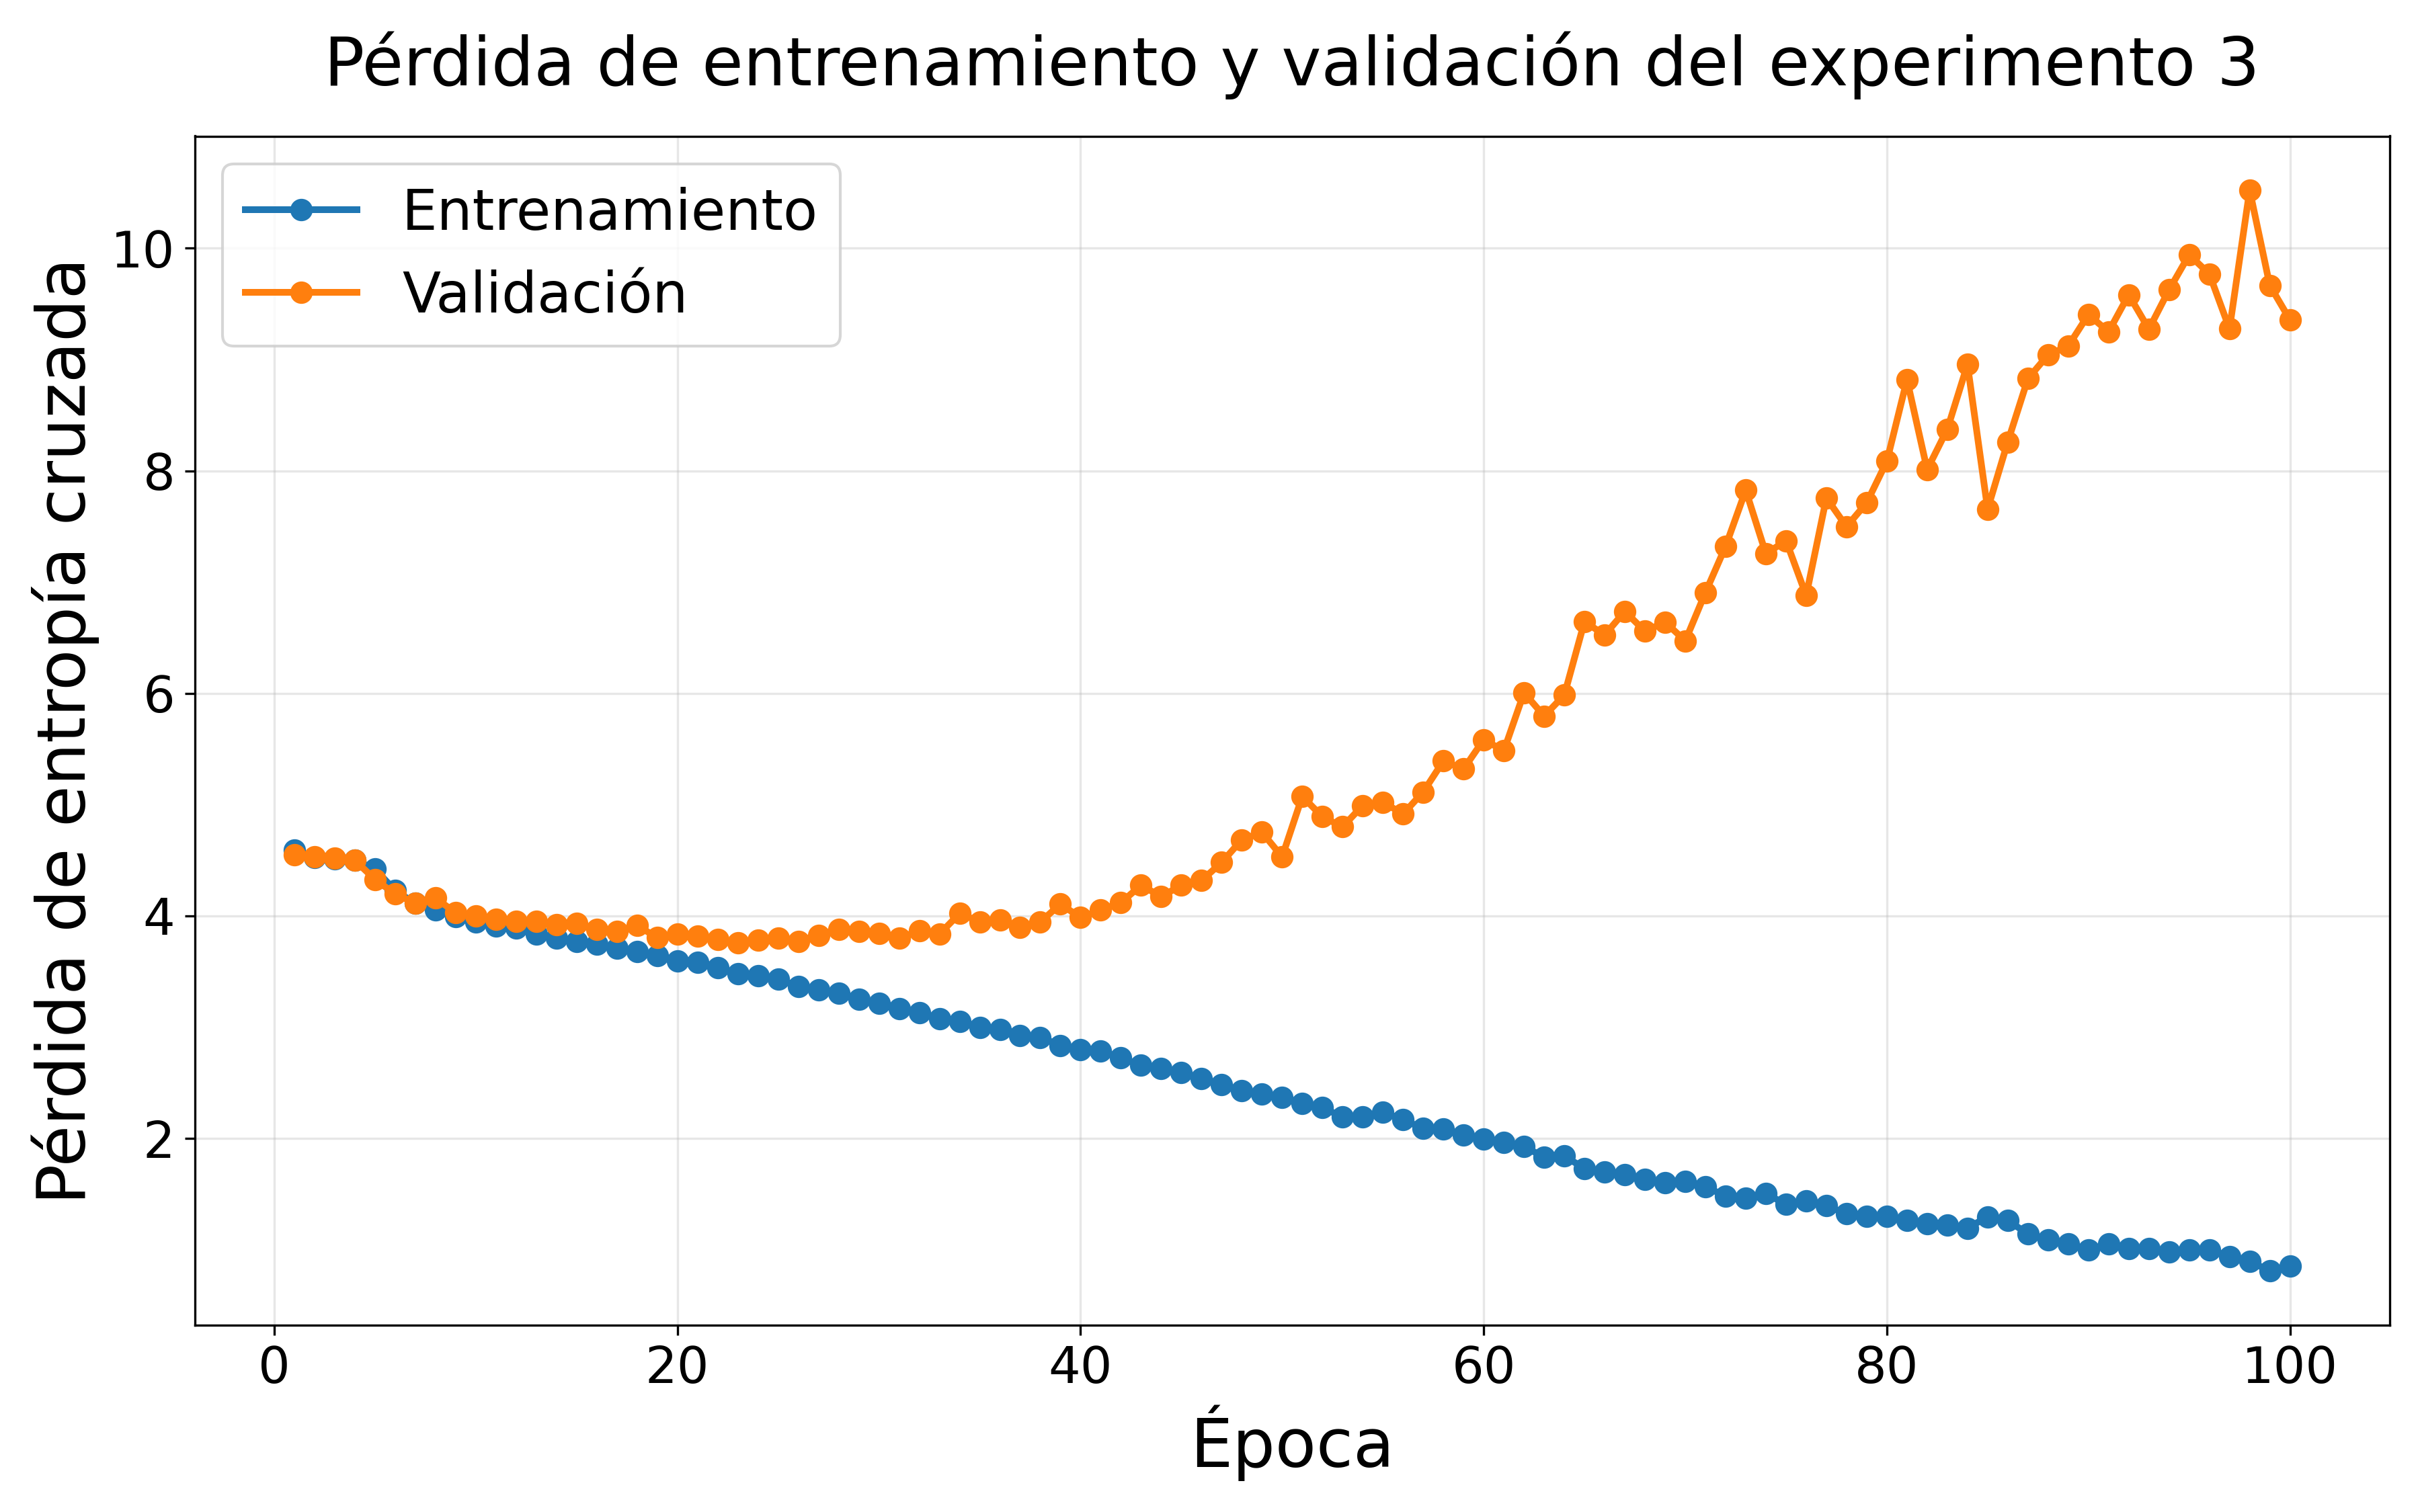
\includegraphics[width=0.55\linewidth]{figures/Experiments_logs/loss_curve_04-27.png}
    \caption{Experimento largo con \texttt{HybridCustomTTN} sobre Flowers102.}
    \label{fig:loss_curve_04-27}
\end{figure}

\begin{table}[H]
\centering
\small
\begin{tabular}{lccccc}
\toprule
\textbf{Experimento} & \textbf{Acc. eval} & \textbf{Época} & \textbf{Train loss} & \textbf{Eval loss} & \textbf{Acc. final} \\
\midrule
\texttt{3} & 12,46\% & 54 & 1,3295 & 8,2368 & 8,55\% \\
\bottomrule
\end{tabular}
\caption{Resumen del experimento largo con \texttt{HybridCustomTTN}.}
\label{tab:hybridttn_largo}
\end{table}

Aquí ya se ve mucho mejor el problema. La \textit{train loss} baja de forma sostenida hasta 1,3295, así que el modelo sí aprende el conjunto de entrenamiento. Sin embargo, la \textit{eval loss} sube hasta 8,2368 y la precisión final cae al 8,55\%. Esto es una señal clara de \textit{overfitting}, el modelo se adapta al entrenamiento, pero no generaliza bien a imágenes nuevas.

\subsection{Hipótesis 2}

La segunda hipótesis fue que el modelo estaba perdiendo demasiada información espacial de la imagen. Hasta ese momento se usaba \texttt{PatchEmbedding}. Para imágenes de $224\times224$ y \texttt{patch\_size=16}, la imagen se divide en una rejilla de $14\times14$, es decir, 196 posiciones. Cada \textit{patch} se proyecta a una dimensión \texttt{local\_dim} y se entrega a la TTN:

\begin{center}
\texttt{[B, 3, 224, 224] -> [B, 196, local\_dim]}.
\end{center}

El problema es que, en las primeras pruebas, \texttt{local\_dim} era muy pequeña. Se estaba comprimiendo cada \textit{patch} de la imagen a muy pocos números antes de que el modelo pudiera procesar bien la localidad espacial. El zigzag ayudaba a ordenar la secuencia, pero no recuperaba la estructura 2D original. Por eso el siguiente cambio fue introducir un \textit{embedding} que procesara la imagen como mapa bidimensional antes de aplanarla.

\section{Cambio del embedding a AIM}

El cambio a \texttt{AIMPatchEmbedding} nace de la hipótesis 2. El objetivo era conservar más información espacial antes de entregar la imagen a la TTN. Para ello se incorporó un \textit{front-end} inspirado en los bloques AIM de \textit{Deep Tree Tensor Networks for Image Recognition} \citebox{nie2025deeptreetensornetworks}.

\begin{center}
\texttt{imagen -> stem CNN -> AIM2D -> Conv2d 1x1 -> flatten + zigzag -> HybridCustomTTN}
\end{center}

El bloque AIM2D combina dos ramas lineales mediante producto elemento a elemento. Si ambas ramas son lineales en la entrada, su producto introduce interacciones bilineales. Esta idea encaja muy bien con las redes tensoriales, porque introduce interacciones multiplicativas estructuradas antes de pasar a la TTN.

En términos de dimensiones, con imágenes de $224\times224$ y \texttt{patch\_size=16}, el front-end reduce la imagen a una rejilla $14\times14$. Después, una convolución $1\times1$ proyecta los canales a \texttt{local\_dim}, y finalmente la rejilla se aplana:

\begin{center}
\texttt{[B, 3, 224, 224] -> [B, local\_dim, 14, 14] -> [B, 196, local\_dim]}.
\end{center}

El primer experimento con AIM durante 50 épocas fue:

\begin{figure}[H]
    \centering
    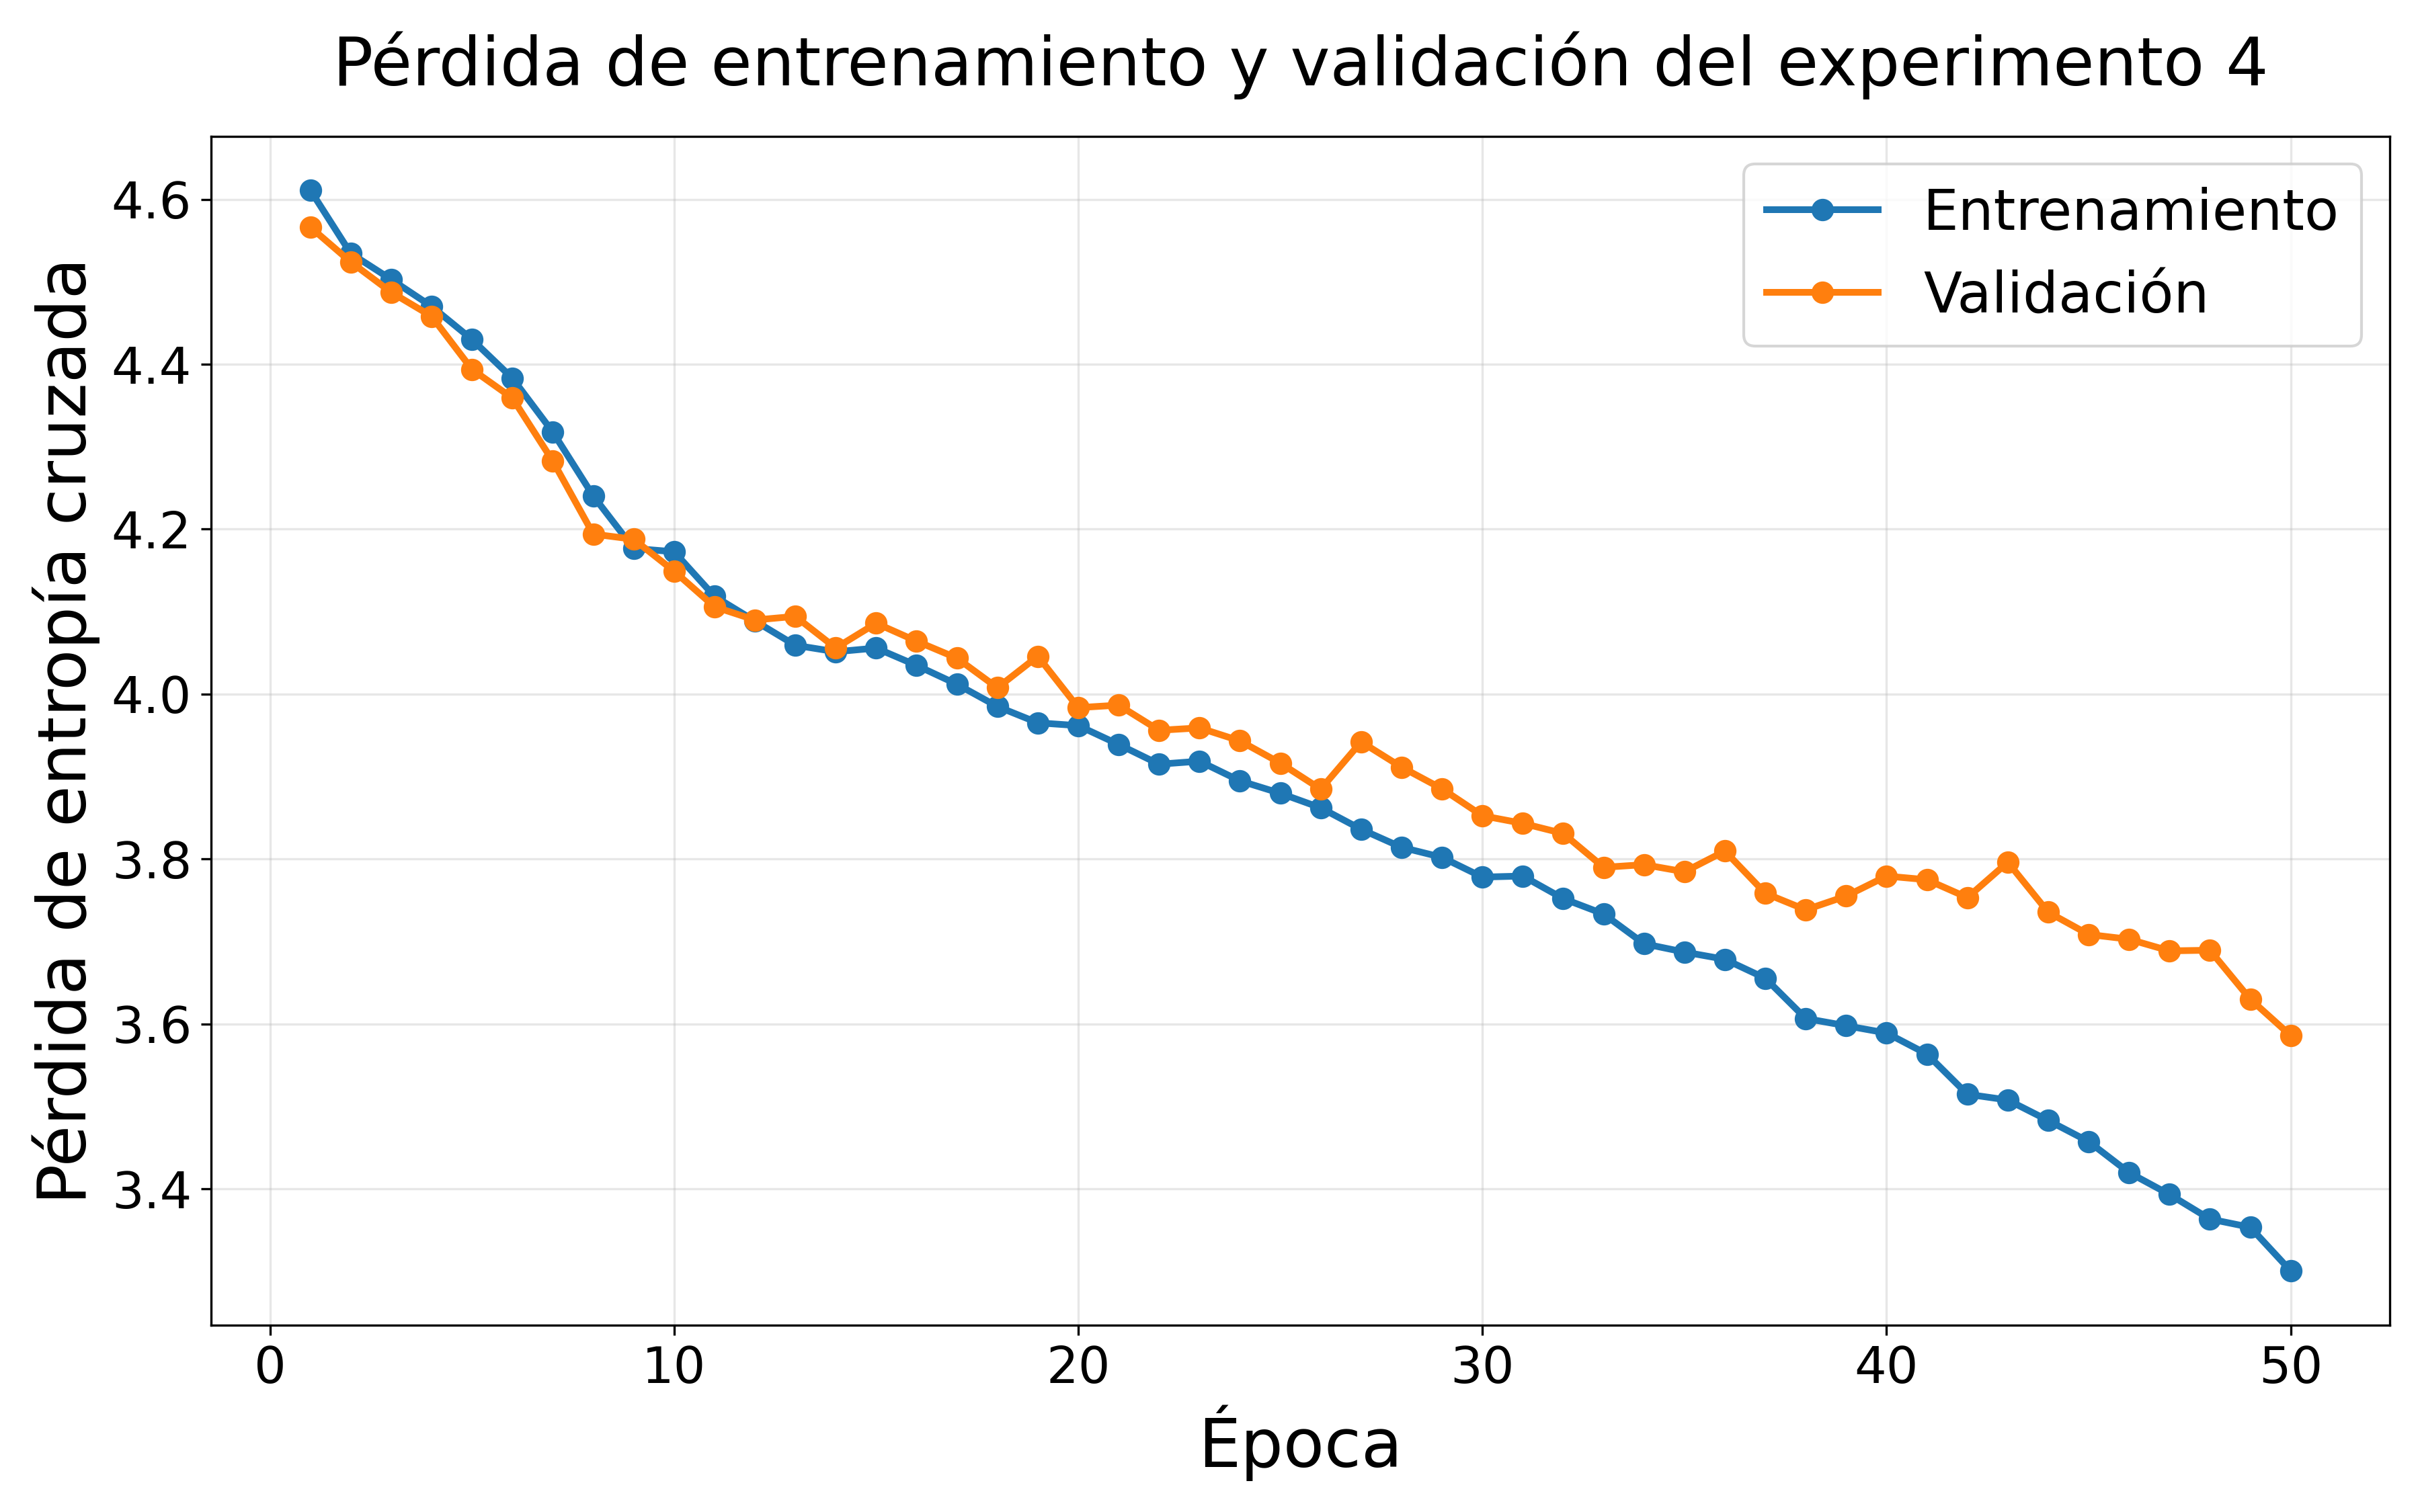
\includegraphics[width=0.55\linewidth]{figures/Experiments_logs/loss_curve_04-28-50.png}
    \caption{Experimento con \texttt{AIMPatchEmbedding} durante 50 épocas.}
    \label{fig:loss_curve_04-28-50}
\end{figure}

\begin{table}[H]
\centering
\small
\begin{tabular}{lcccc}
\toprule
\textbf{Experimento} & \textbf{Épocas} & \textbf{Mejor acc. eval} & \textbf{Mejor eval loss} & \textbf{Acc. final} \\
\midrule
\texttt{4} & 50 & 14,01\% & 3,5859 & 14,01\% \\
\bottomrule
\end{tabular}
\caption{Primer resultado con \texttt{AIMPatchEmbedding}.}
\label{tab:aim_50}
\end{table}

El resultado fue positivo porque la pérdida seguía bajando y no se observaba una separación tan violenta entre entrenamiento y evaluación. Para compararlo mejor con los experimentos anteriores, se repitió con 100 épocas:

\begin{figure}[H]
    \centering
    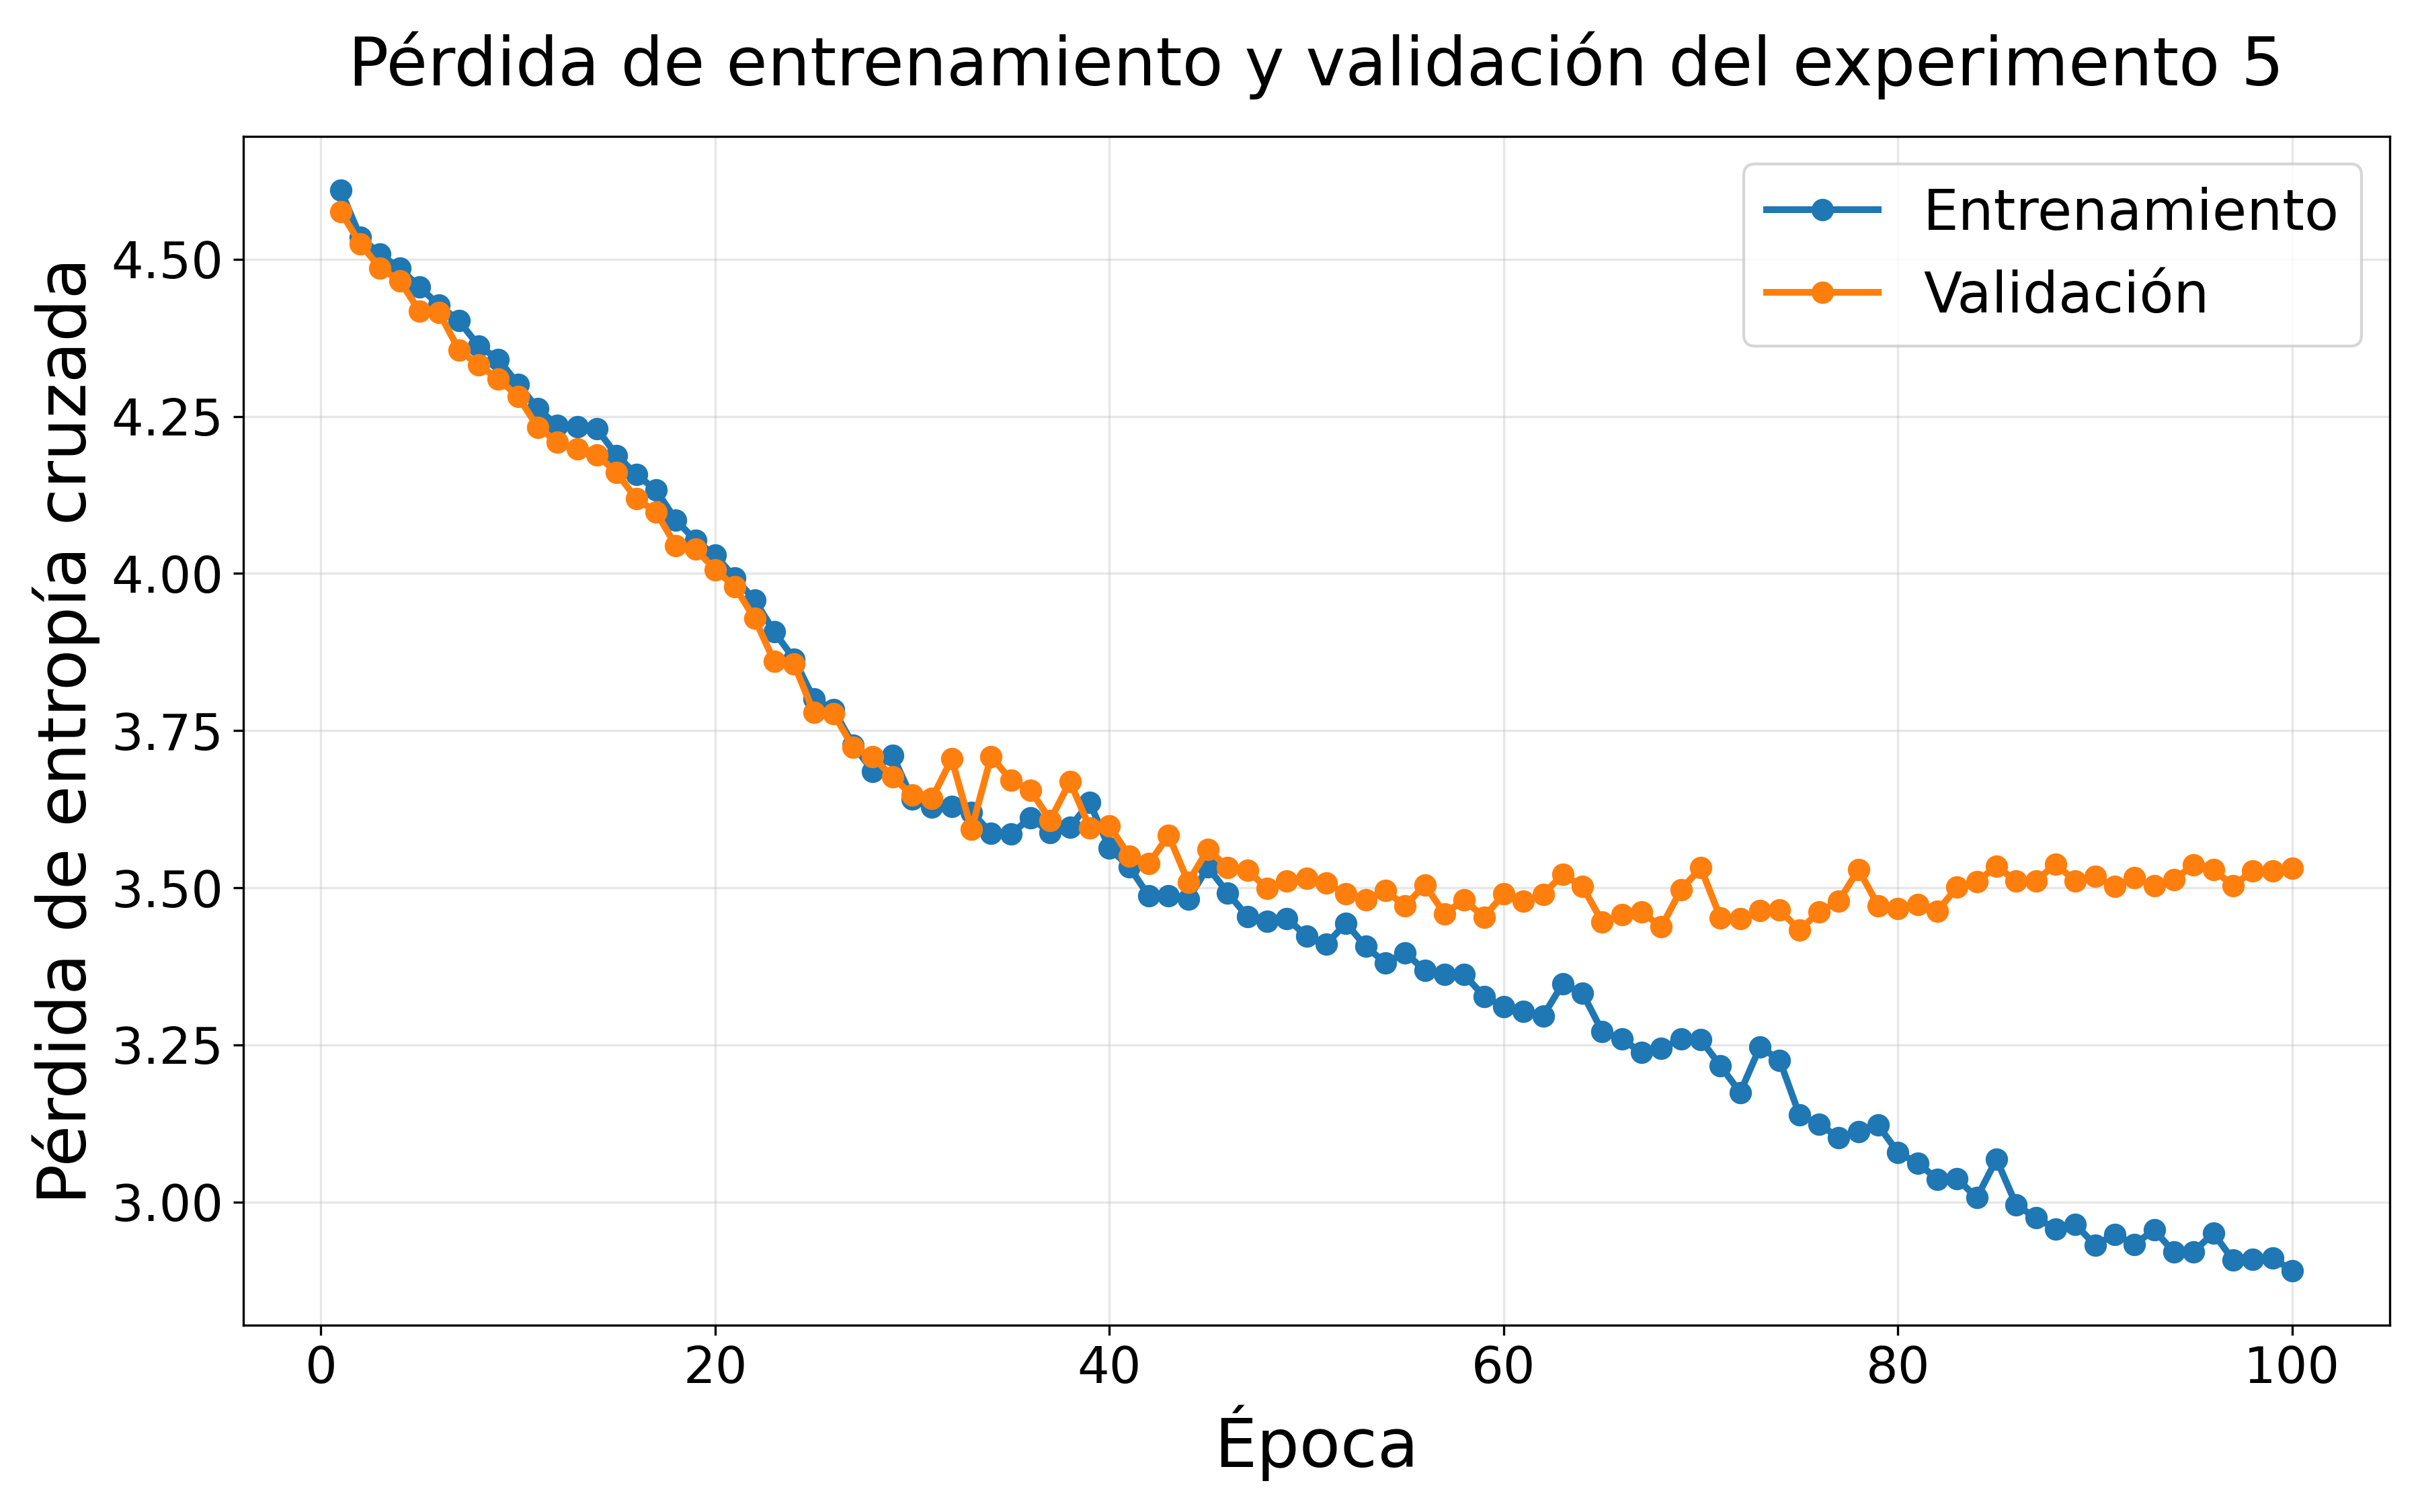
\includegraphics[width=0.55\linewidth]{figures/Experiments_logs/loss_curve_04-28-100.png}
    \caption{Experimento con \texttt{AIMPatchEmbedding} durante 100 épocas.}
    \label{fig:loss_curve_04-28-100}
\end{figure}

\begin{table}[H]
\centering
\small
\begin{tabular}{lcccc}
\toprule
\textbf{Experimento} & \textbf{Épocas} & \textbf{Mejor acc. eval} & \textbf{Mejor eval loss} & \textbf{Eval loss final} \\
\midrule
\texttt{5} & 100 & 15,88\% & 3,4330 & 3,5312 \\
\bottomrule
\end{tabular}
\caption{Resultado con AIM durante 100 épocas.}
\label{tab:aim_100}
\end{table}

Comparado con \figref{fig:loss_curve_04-27}, el \textit{overfitting} ya no era tan agresivo. Antes la \textit{eval loss} acababa en 8,2368, mientras que con AIM se mantuvo alrededor de 3,5312. La precisión seguía siendo baja, pero el comportamiento del entrenamiento era más sano. Esto indicaba que AIM no era una solución mágica, pero sí estaba atacando el problema correcto.

El siguiente paso fue aplicar \textit{data augmentation}. Esta técnica consiste en generar variaciones de las imágenes durante el entrenamiento, por ejemplo con cambios de recorte, color, orientación o borrado parcial. La idea es que el modelo no memorice una única versión de cada imagen, sino que aprenda rasgos más generales.

\begin{figure}[H]
    \centering

    \begin{subfigure}{0.45\textwidth}
        \centering
        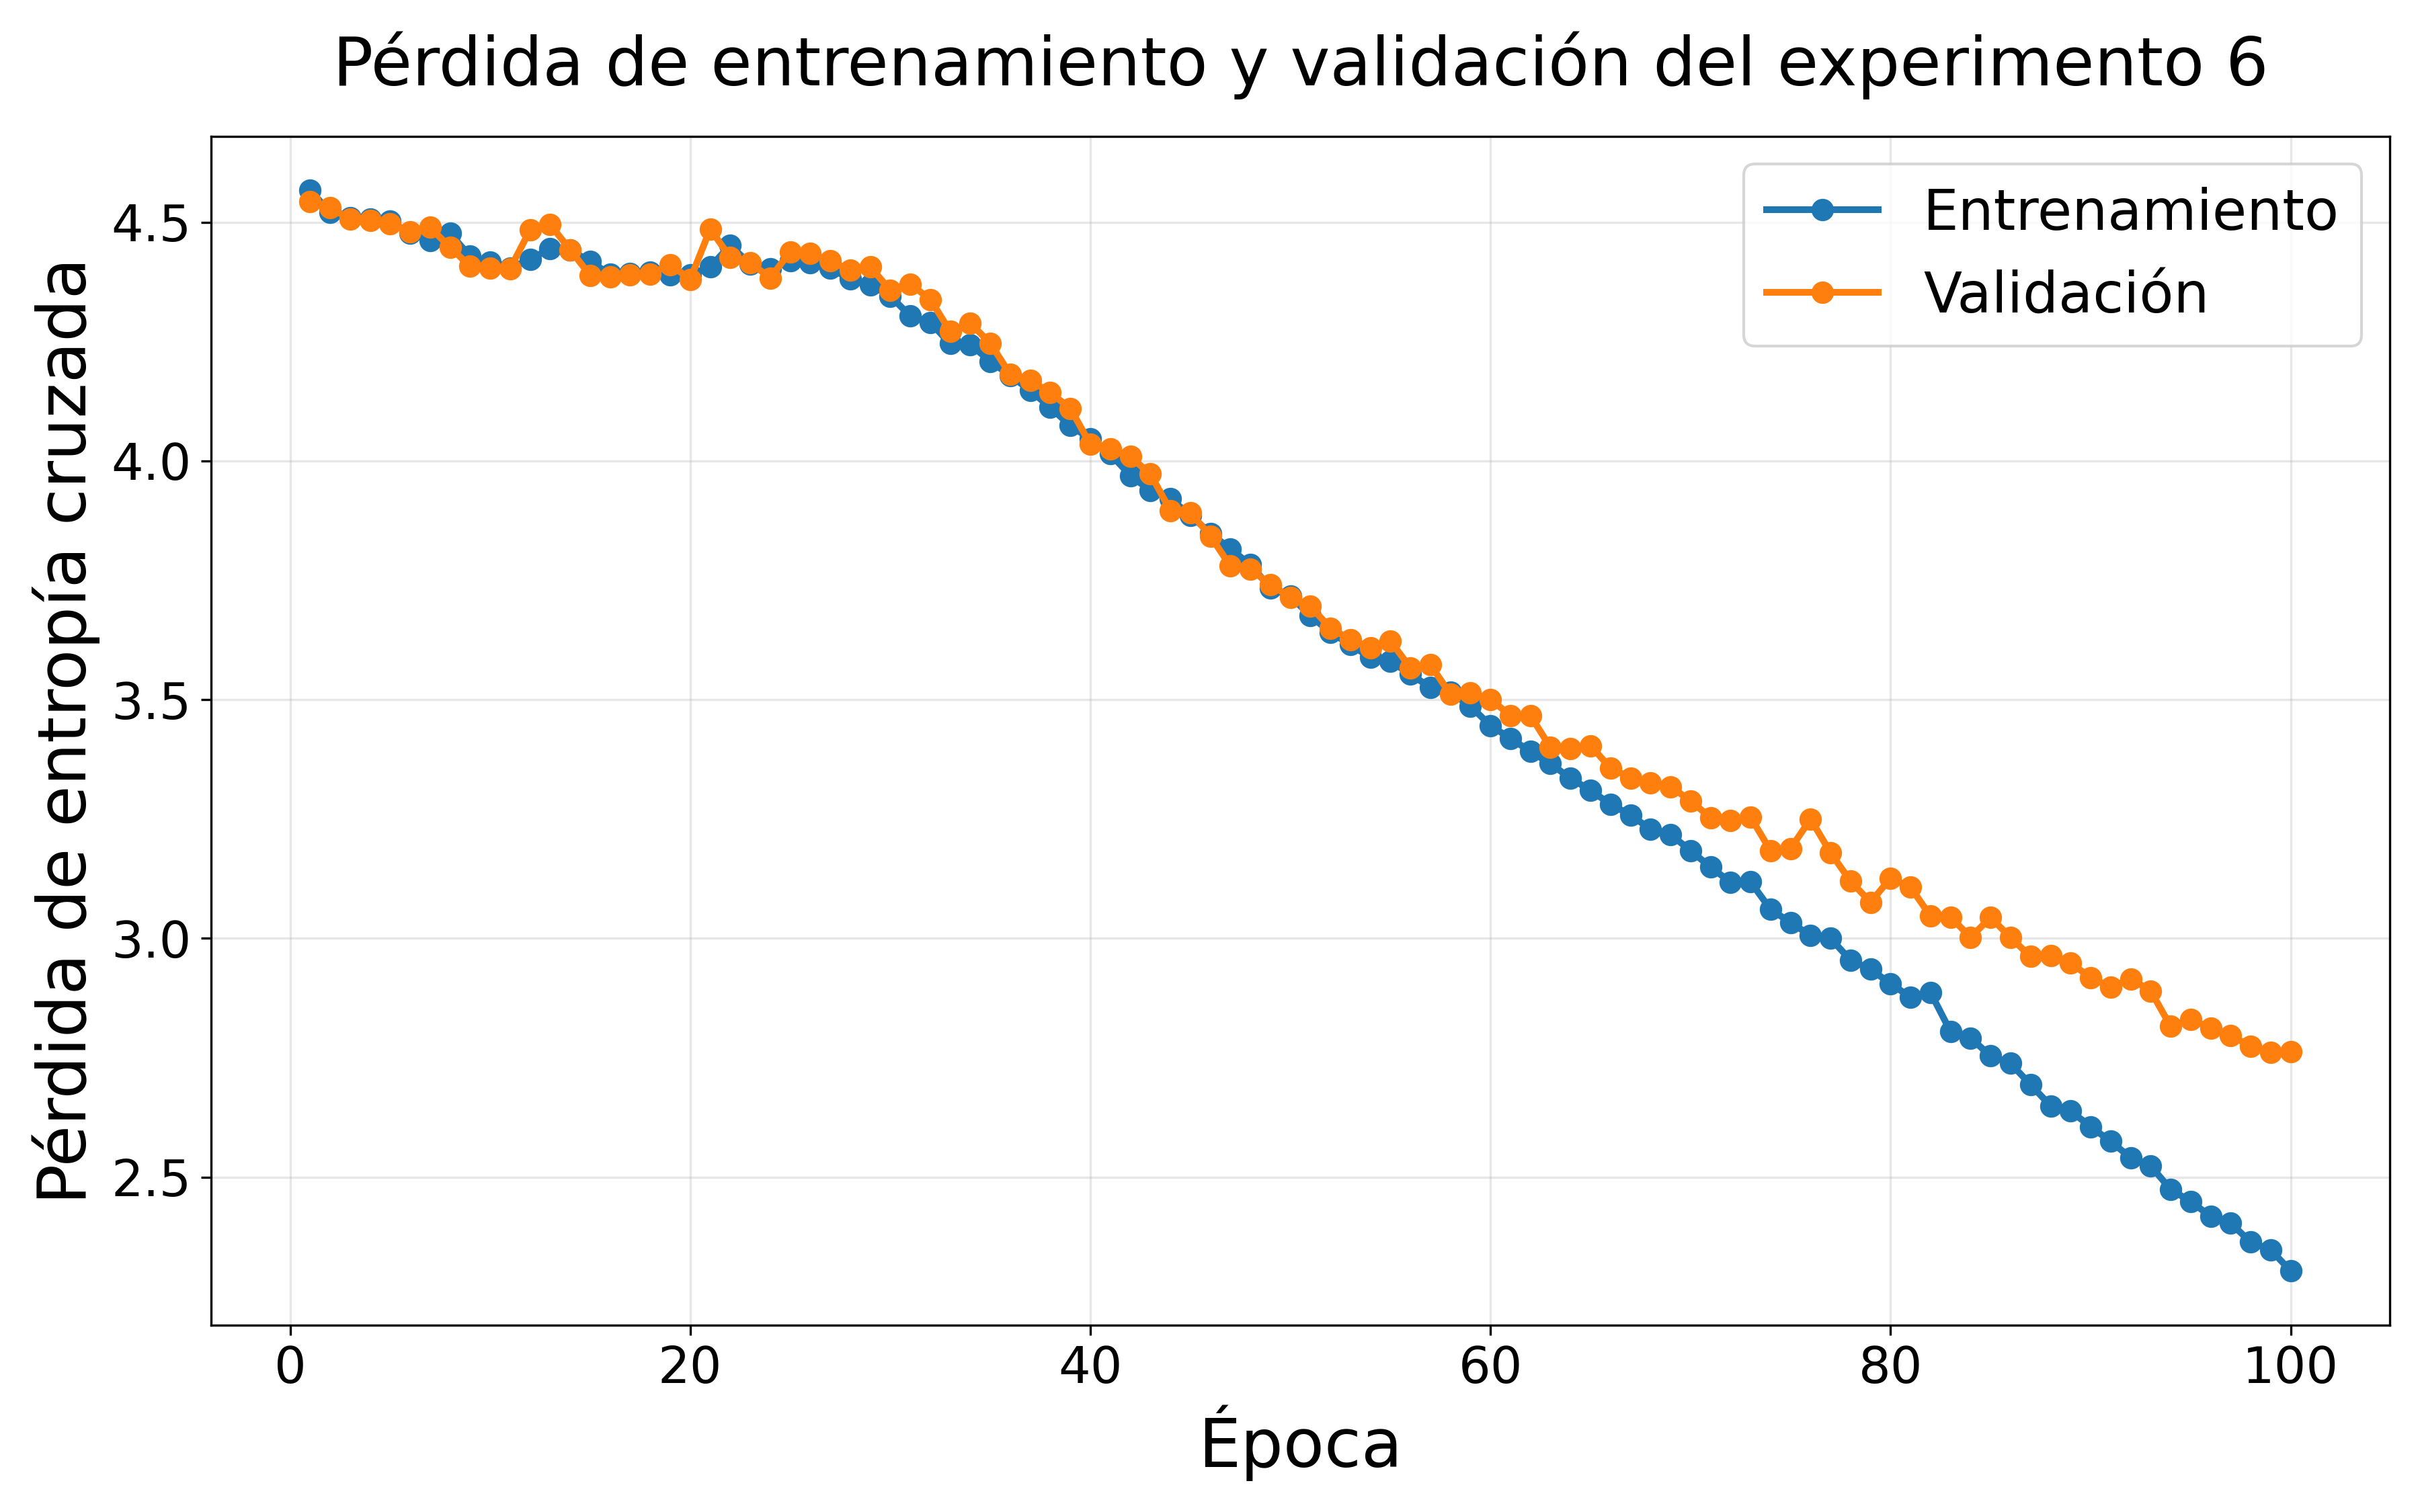
\includegraphics[width=\textwidth]{figures/Experiments_logs/loss_curve_04-30-0011.png}
        \caption{}
        \label{fig:loss_curve_04-30-0011}
    \end{subfigure}
    \hfill
    \begin{subfigure}{0.45\textwidth}
        \centering
        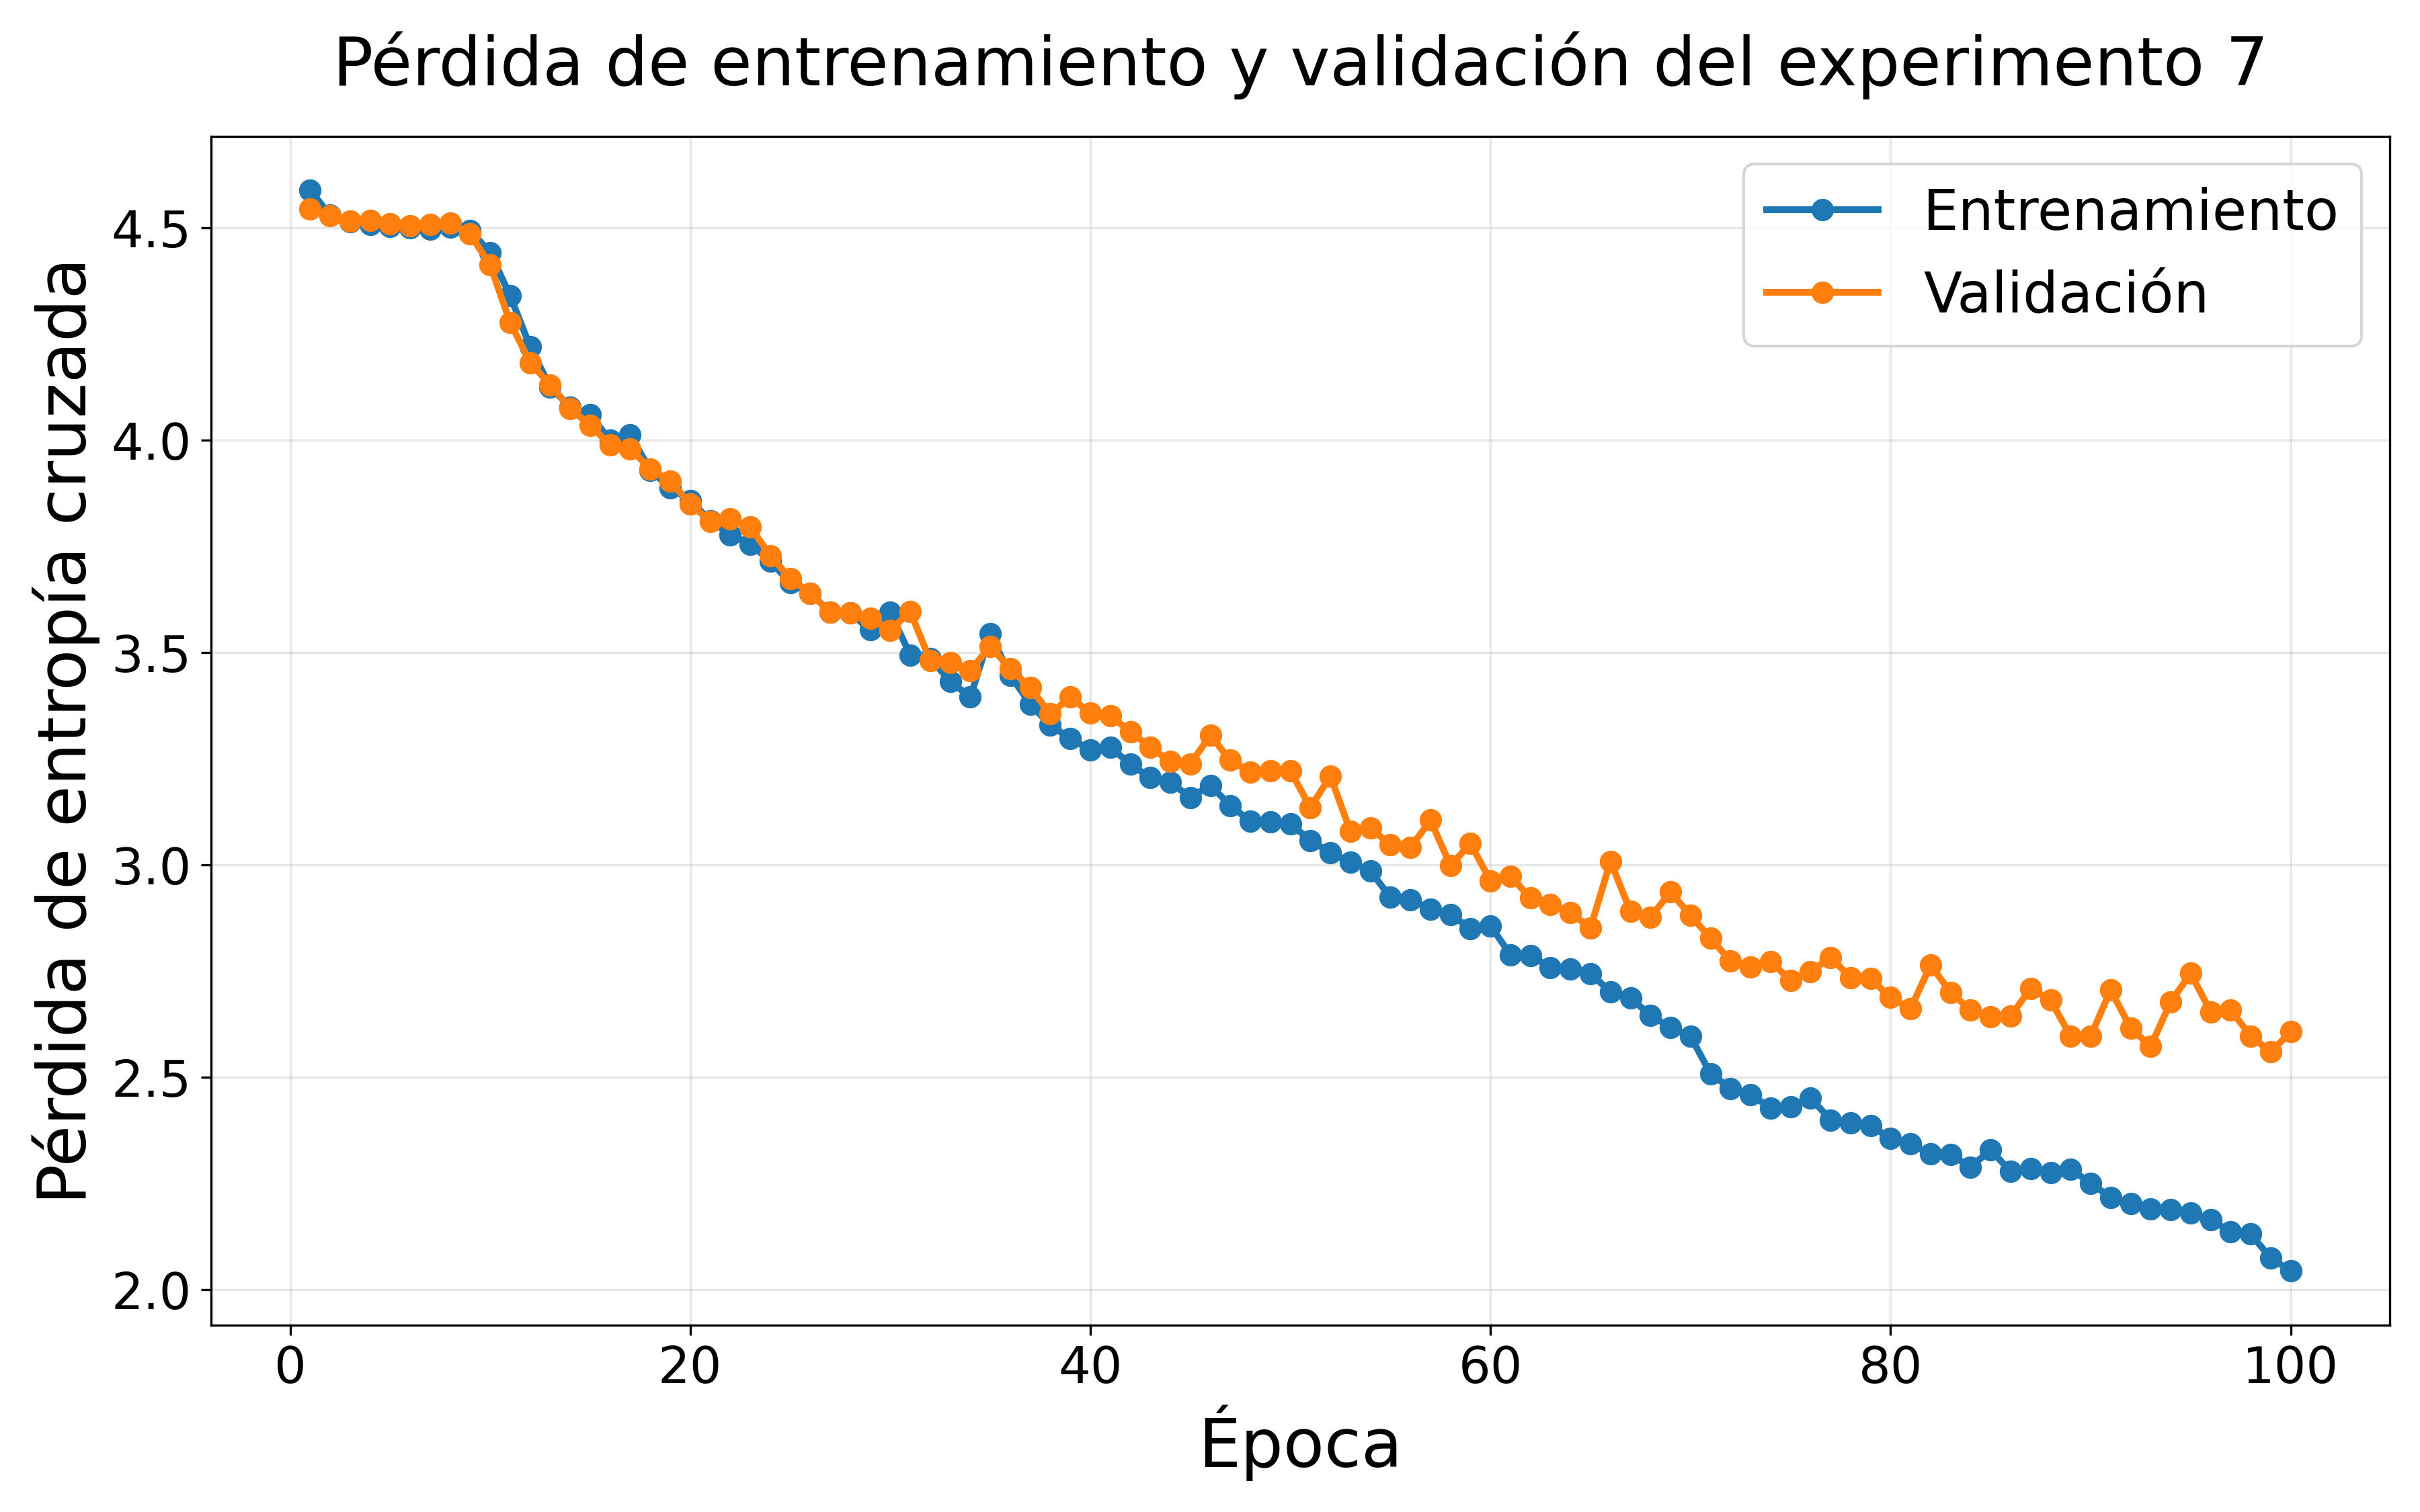
\includegraphics[width=\textwidth]{figures/Experiments_logs/loss_curve_04-30-0021.png}
        \caption{}
        \label{fig:loss_curve_04-30-0021}
    \end{subfigure}

    \caption{Experimentos en Flowers102 con AIM y \textit{data augmentation}.}
    \label{fig:loss_curve_04-30-0011-0021}
\end{figure}

\begin{table}[H]
\centering
\small
\begin{tabular}{lcccc}
\toprule
\textbf{Experimento} & \textbf{Mejor acc. eval} & \textbf{Top-5 eval} & \textbf{Mejor eval loss} & \textbf{Acc. final} \\
\midrule
\texttt{6} & 30,13\% & 61,40\% & 2,7612 & 29,97\% \\
\texttt{7} & 33,96\% & 66,04\% & 2,5600 & 33,96\% \\
\bottomrule
\end{tabular}
\caption{Mejores resultados sobre Flowers102 después de añadir AIM y \textit{data augmentation}.}
\label{tab:flowers_aim_aug}
\end{table}

Aquí el cambio ya fue bastante más claro. La precisión subió hasta 33,96\% y el top-5 alcanzó 66,04\%. Aun así, la matriz de confusión mostraba que el modelo seguía confundiendo muchas clases.

\begin{figure}[H]
    \centering

    \begin{subfigure}{0.45\textwidth}
        \centering
        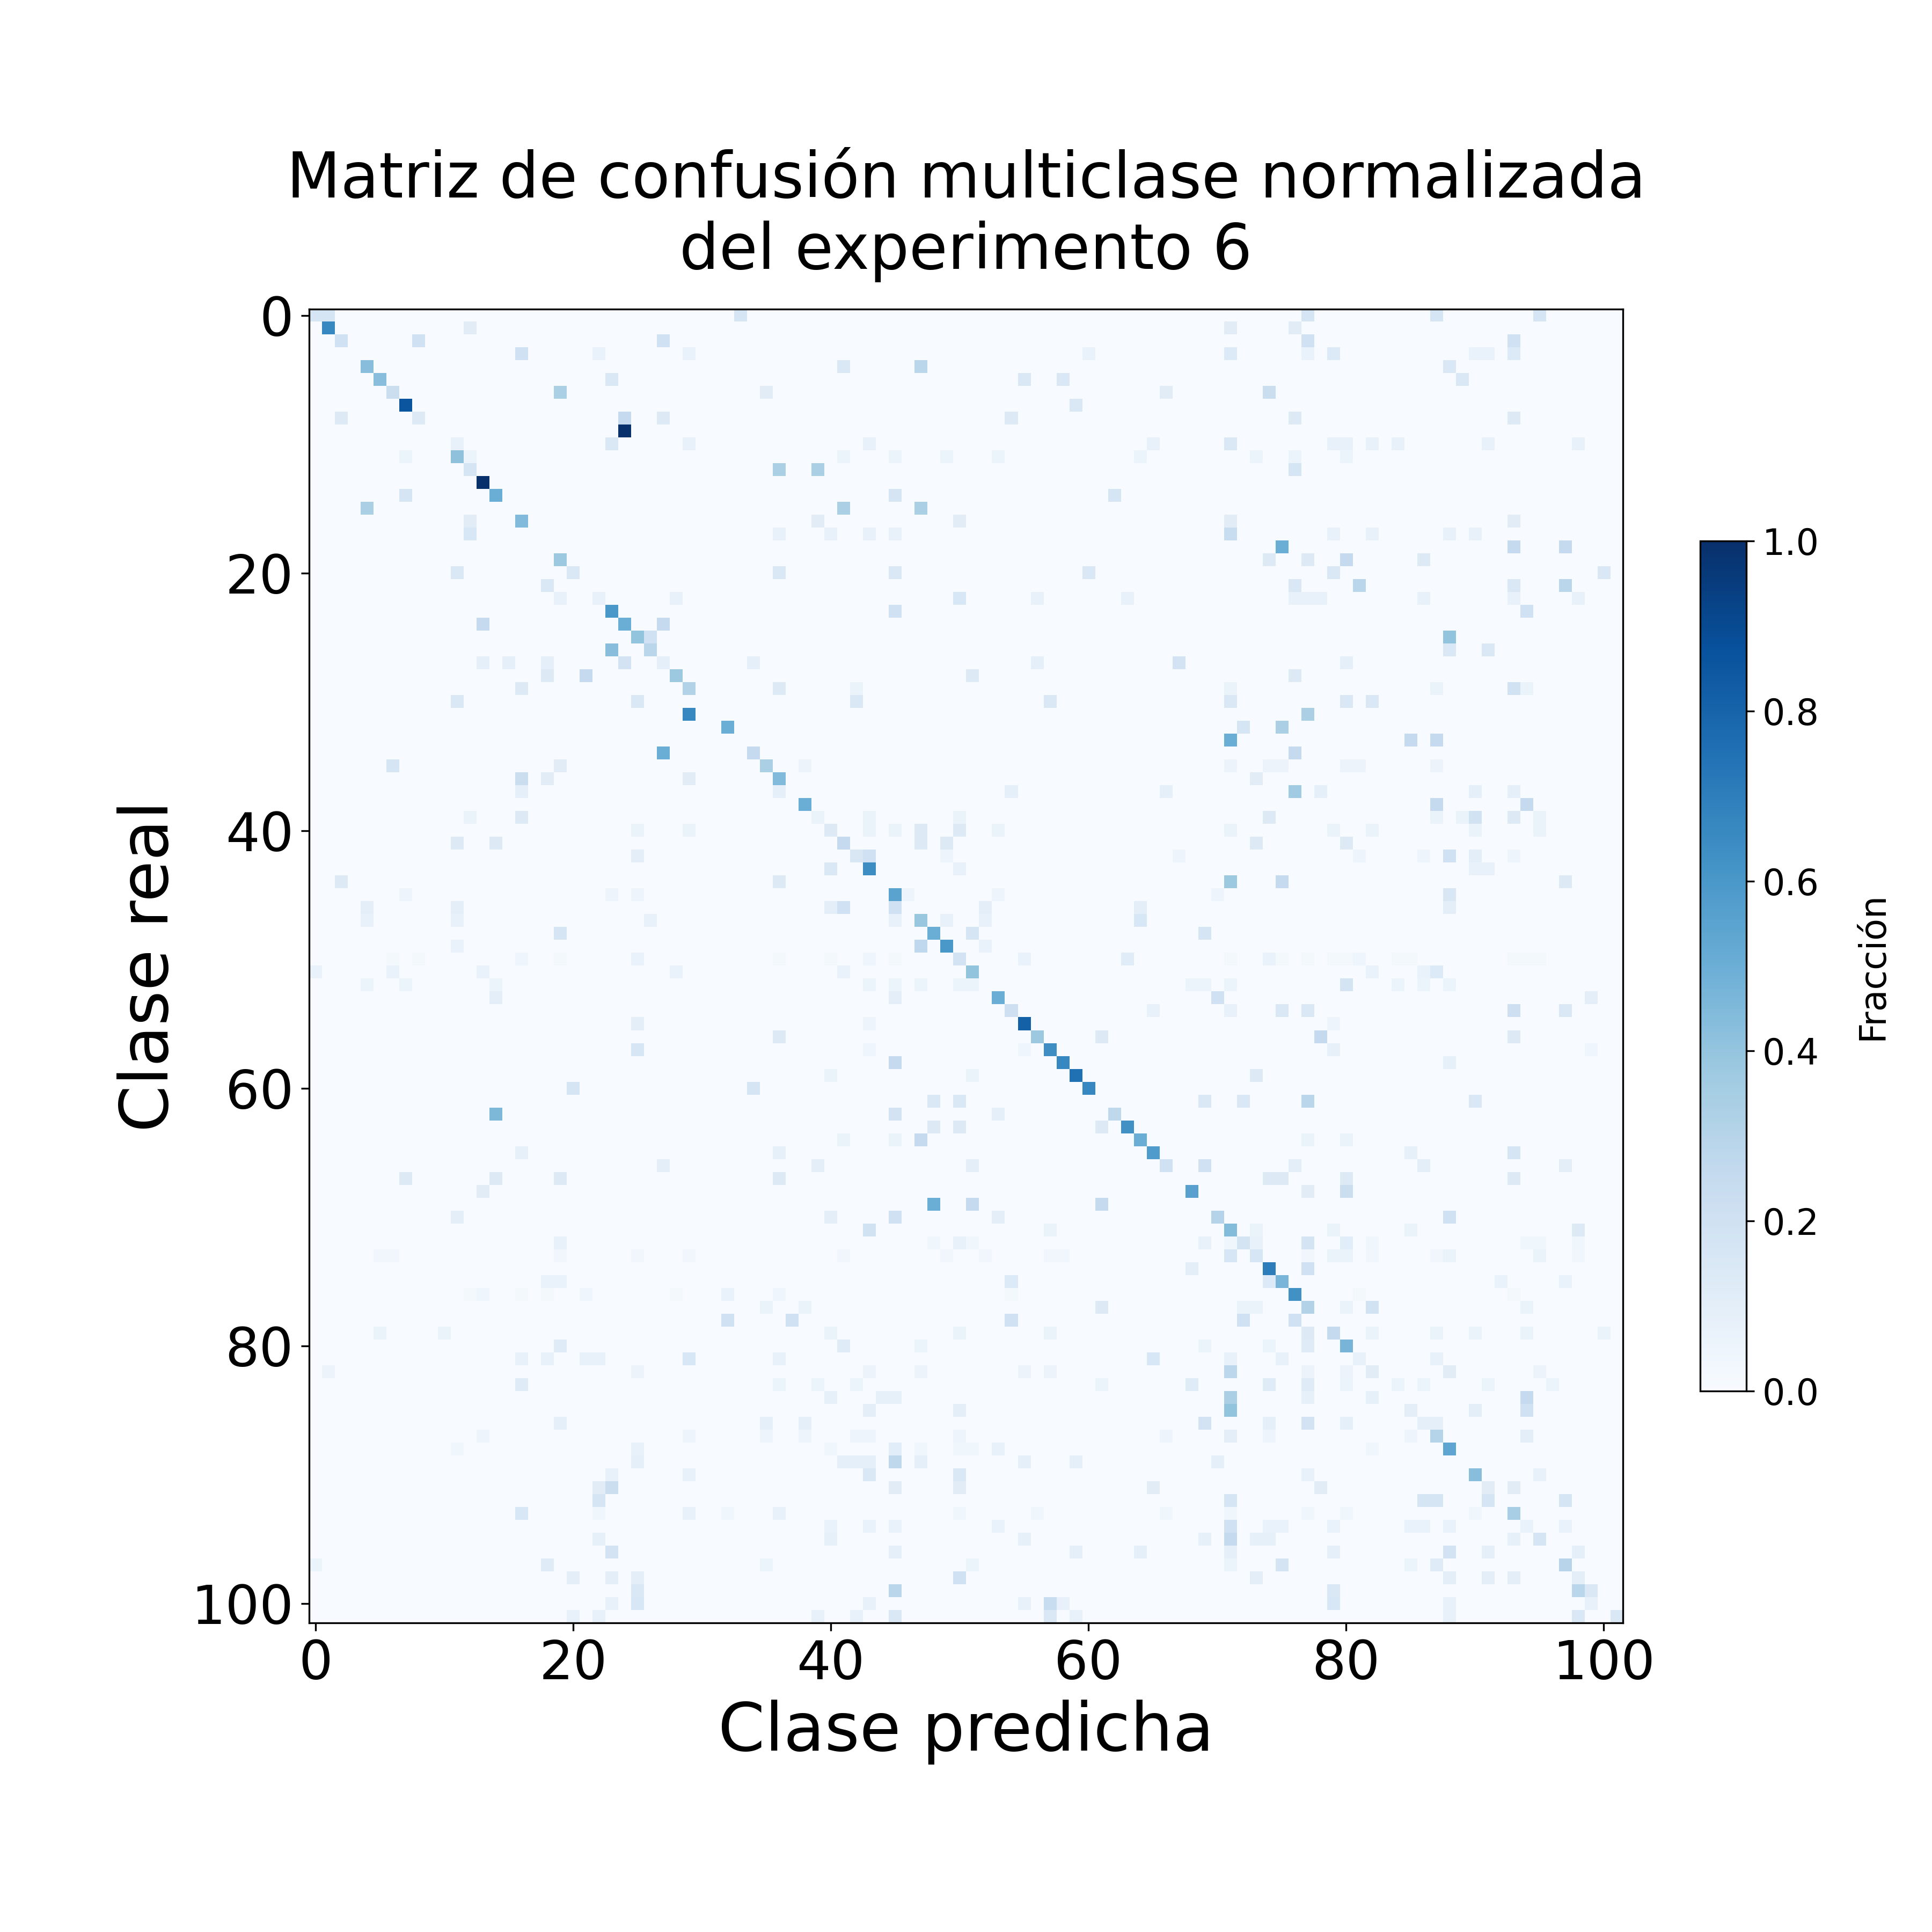
\includegraphics[width=\textwidth]{figures/Experiments_logs/confusion_matrix_04-30-0011.png}
        \caption{}
        \label{fig:confusion_matrix_04-30-0011}
    \end{subfigure}
    \hfill
    \begin{subfigure}{0.45\textwidth}
        \centering
        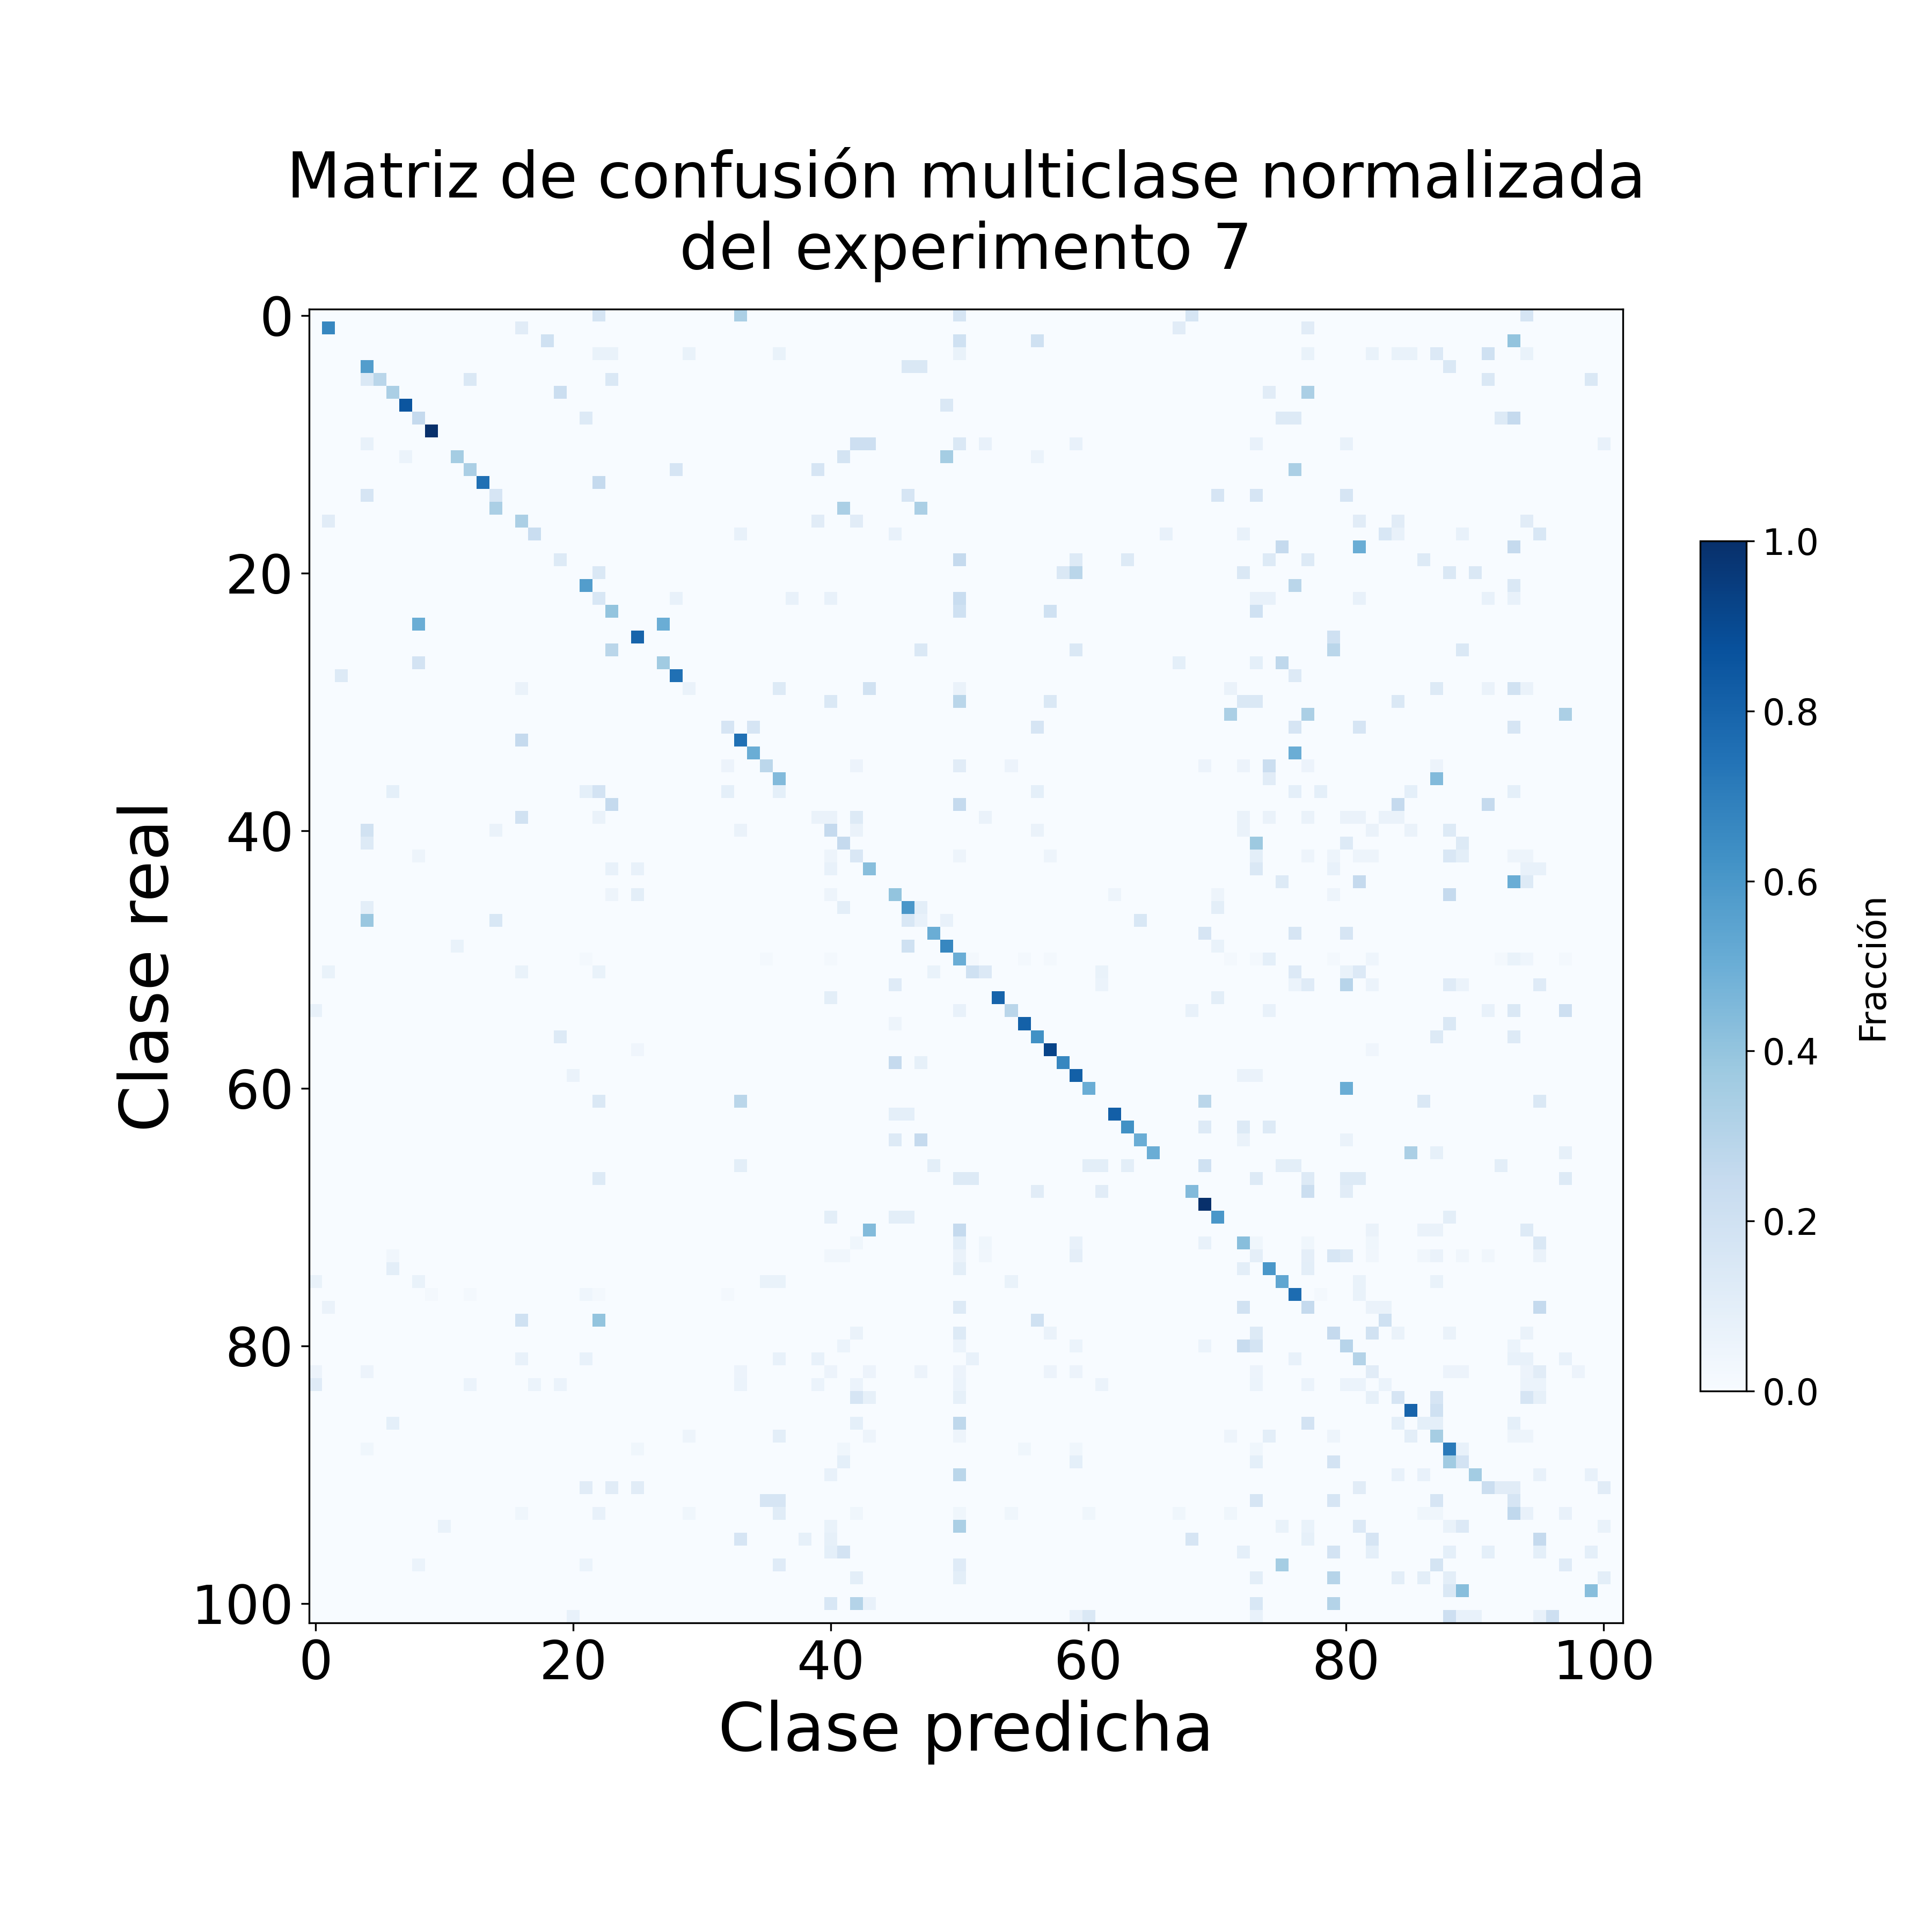
\includegraphics[width=\textwidth]{figures/Experiments_logs/confusion_matrix_04-30-0021.png}
        \caption{}
        \label{fig:confusion_matrix_04-30-0021}
    \end{subfigure}

    \caption{Matrices de confusión multiclase en Flowers102 tras AIM y \textit{data augmentation}.}
    \label{fig:confusion_matrix_04-30-0011-0021}
\end{figure}

En una matriz de confusión ideal se vería casi todo concentrado en la diagonal. En este caso la diagonal ya aparece, lo cual significa que el modelo no está prediciendo completamente al azar, pero sigue habiendo muchos valores fuera de ella. Esto llevó a la tercera hipótesis.

\subsection{Hipótesis 3}

La tercera hipótesis fue que el problema ya no era solo que el modelo no aprendiera, sino que Flowers102 era un dataset difícil para esta fase del proyecto. Tiene 102 clases de flores, muchas de ellas visualmente muy parecidas. Incluso para una persona puede ser complicado distinguir correctamente todas las clases sin un conocimiento previo sobre botánica.

Además, Flowers102 nunca fue el objetivo central del TFG. El objetivo era trabajar con imágenes de material de laboratorio, usando ChemEq25. Por tanto, una vez comprobado que el pipeline funcionaba y que AIM mejoraba el comportamiento, el siguiente paso natural fue cambiar al dataset principal.

\section{Cambio de dataset a ChemEq25}

Antes de implementar cualquier dataset en un modelo, es muy importante revisarlo detenidamente. La parte de limpiar y adaptar los datos es una de las más importantes dentro del \textit{machine learning}, porque si los datos no están bien preparados, es muy difícil obtener buenos resultados después.

Revisando ChemEq25 apareció una particularidad importante. Muchas imágenes tenían dimensiones de $640\times640$ píxeles, pero podían contener más de un objeto de laboratorio. Incluso había fotografías con muchos objetos distintos en la misma escena. Si se introdujera una imagen completa en el clasificador, el modelo no sabría qué objeto debe clasificar. Por eso fue necesario usar las anotaciones YOLO del dataset.

Las anotaciones YOLO indican dónde está cada objeto dentro de la imagen. Con ellas se generaron recortes que contienen un único objeto, y cada recorte mantiene su etiqueta correspondiente.

\begin{figure}[H]
    \centering

    \begin{subfigure}{0.45\textwidth}
        \centering
        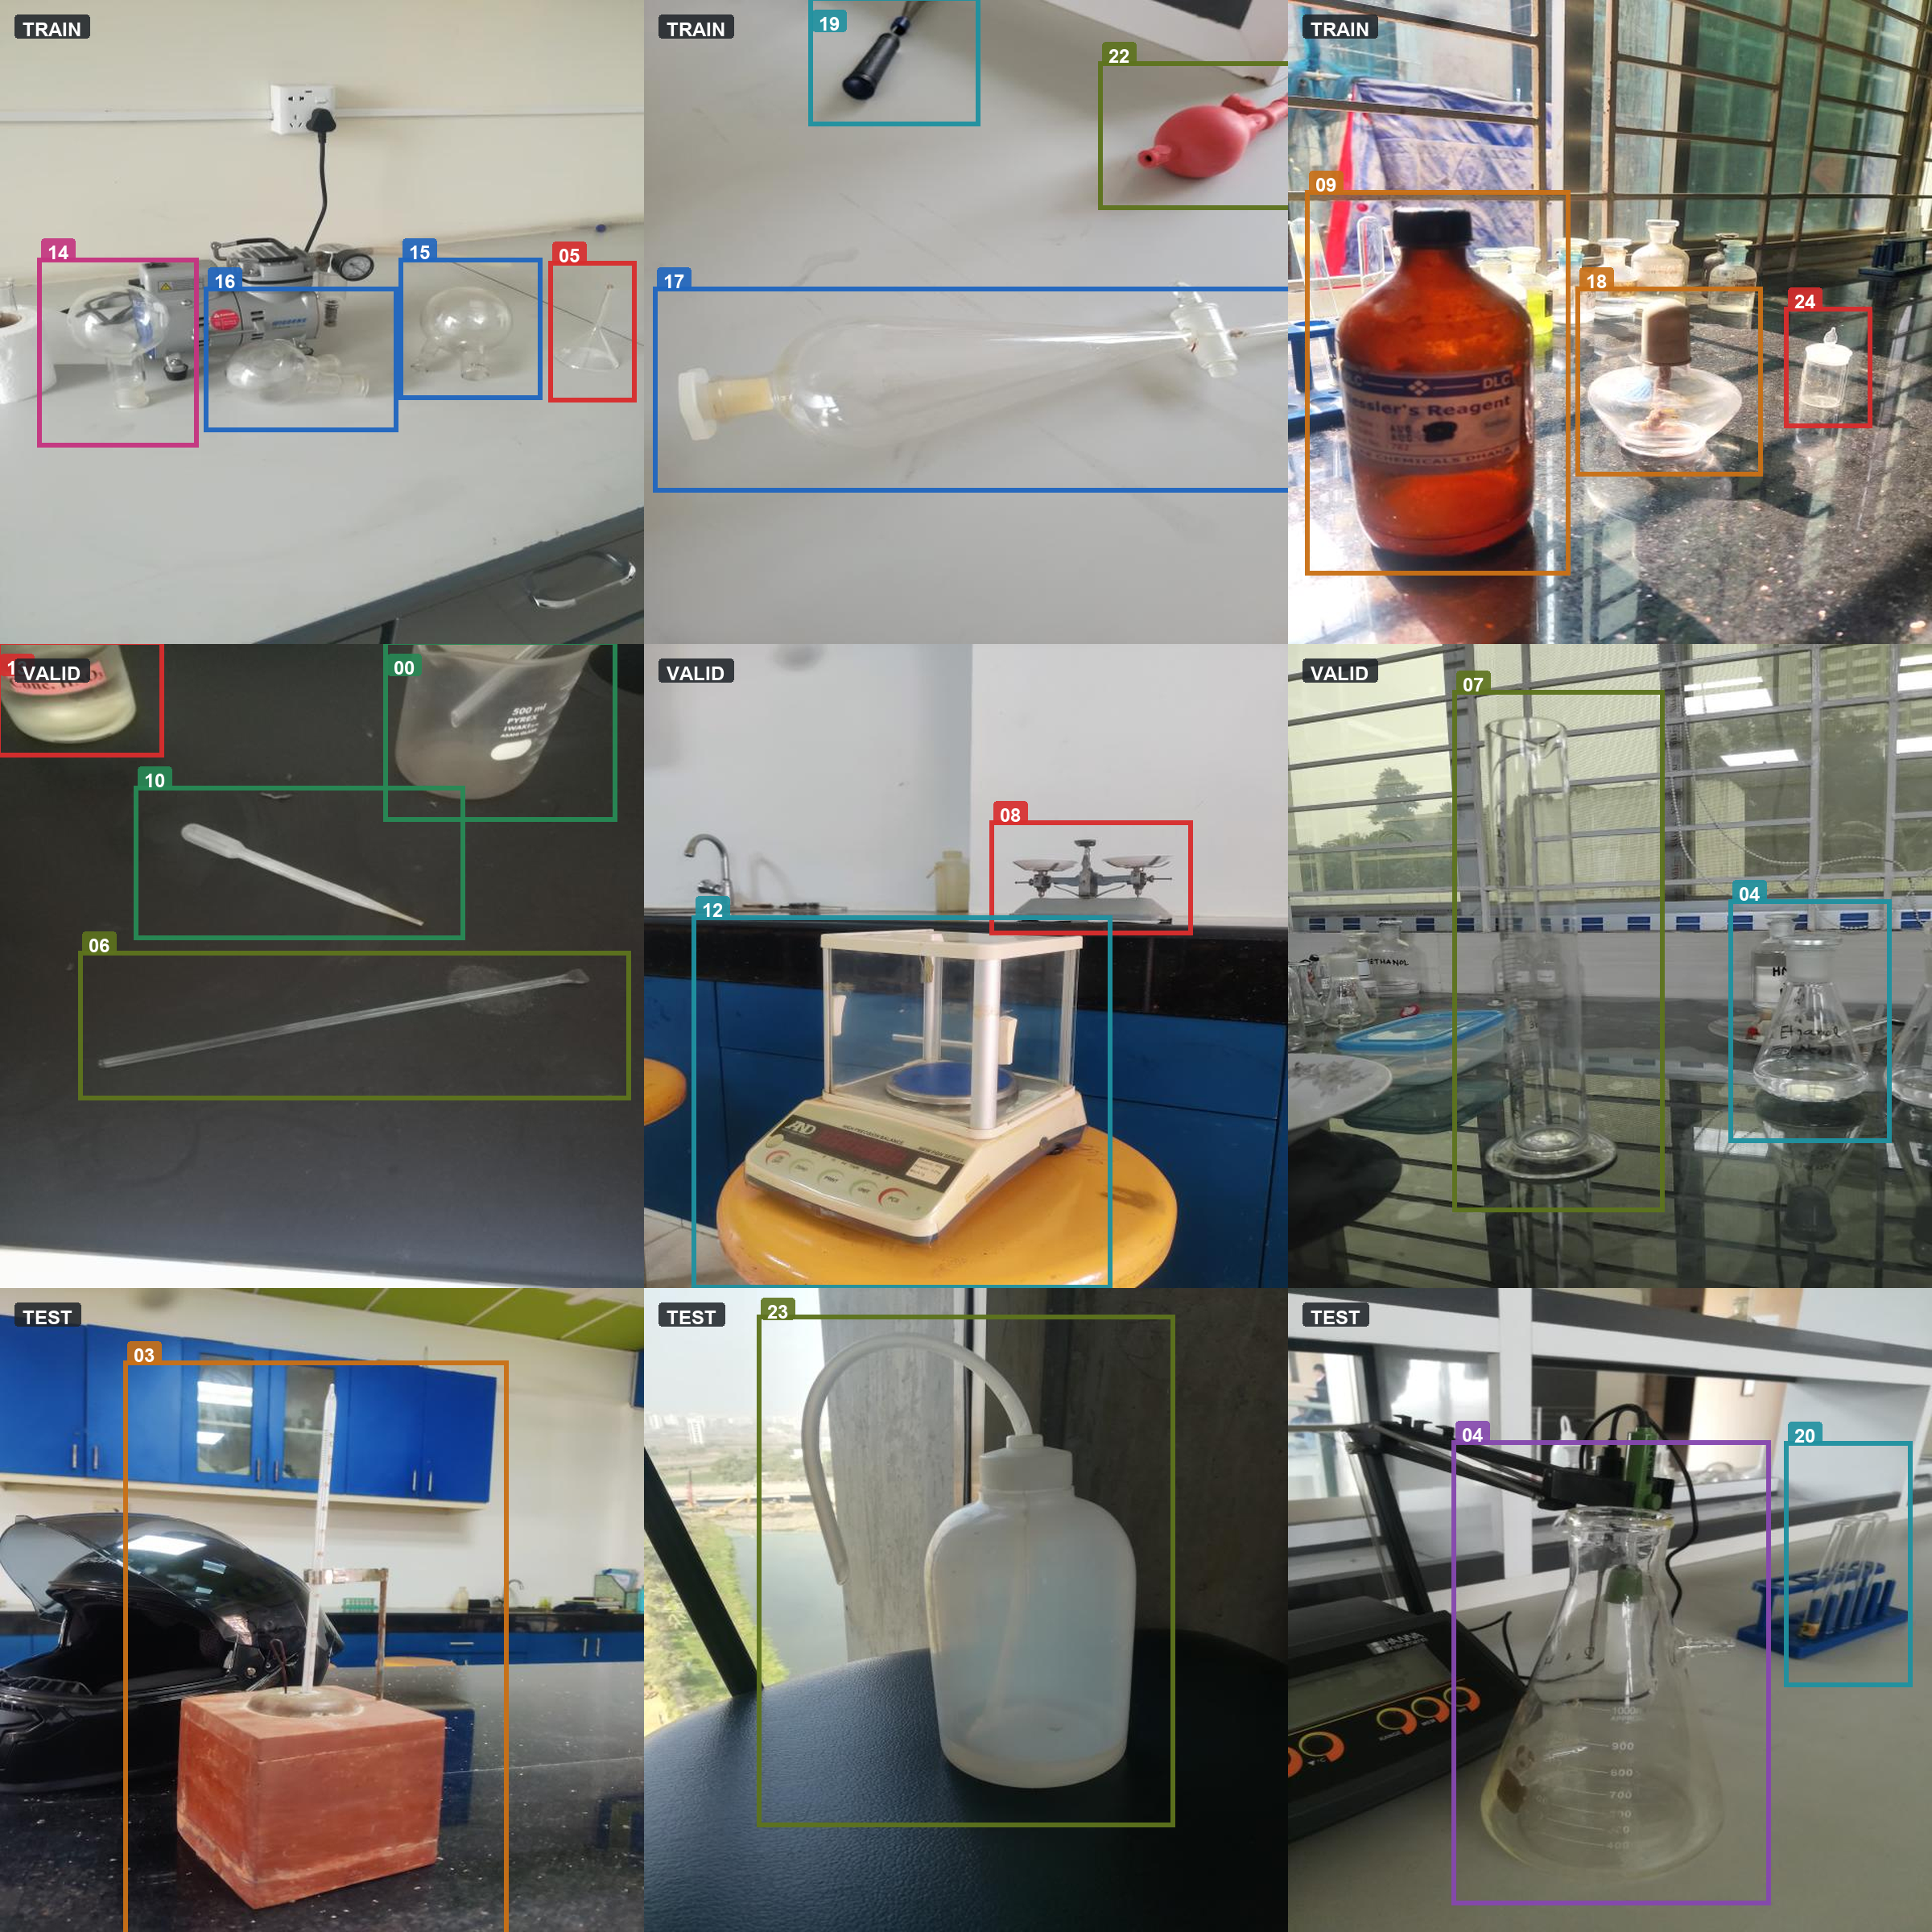
\includegraphics[width=\textwidth]{figures/tfg_dataset_yolo_boxes_square.png}
        \caption{}
        \label{fig:YOLO}
    \end{subfigure}
    \hfill
    \begin{subfigure}{0.45\textwidth}
        \centering
        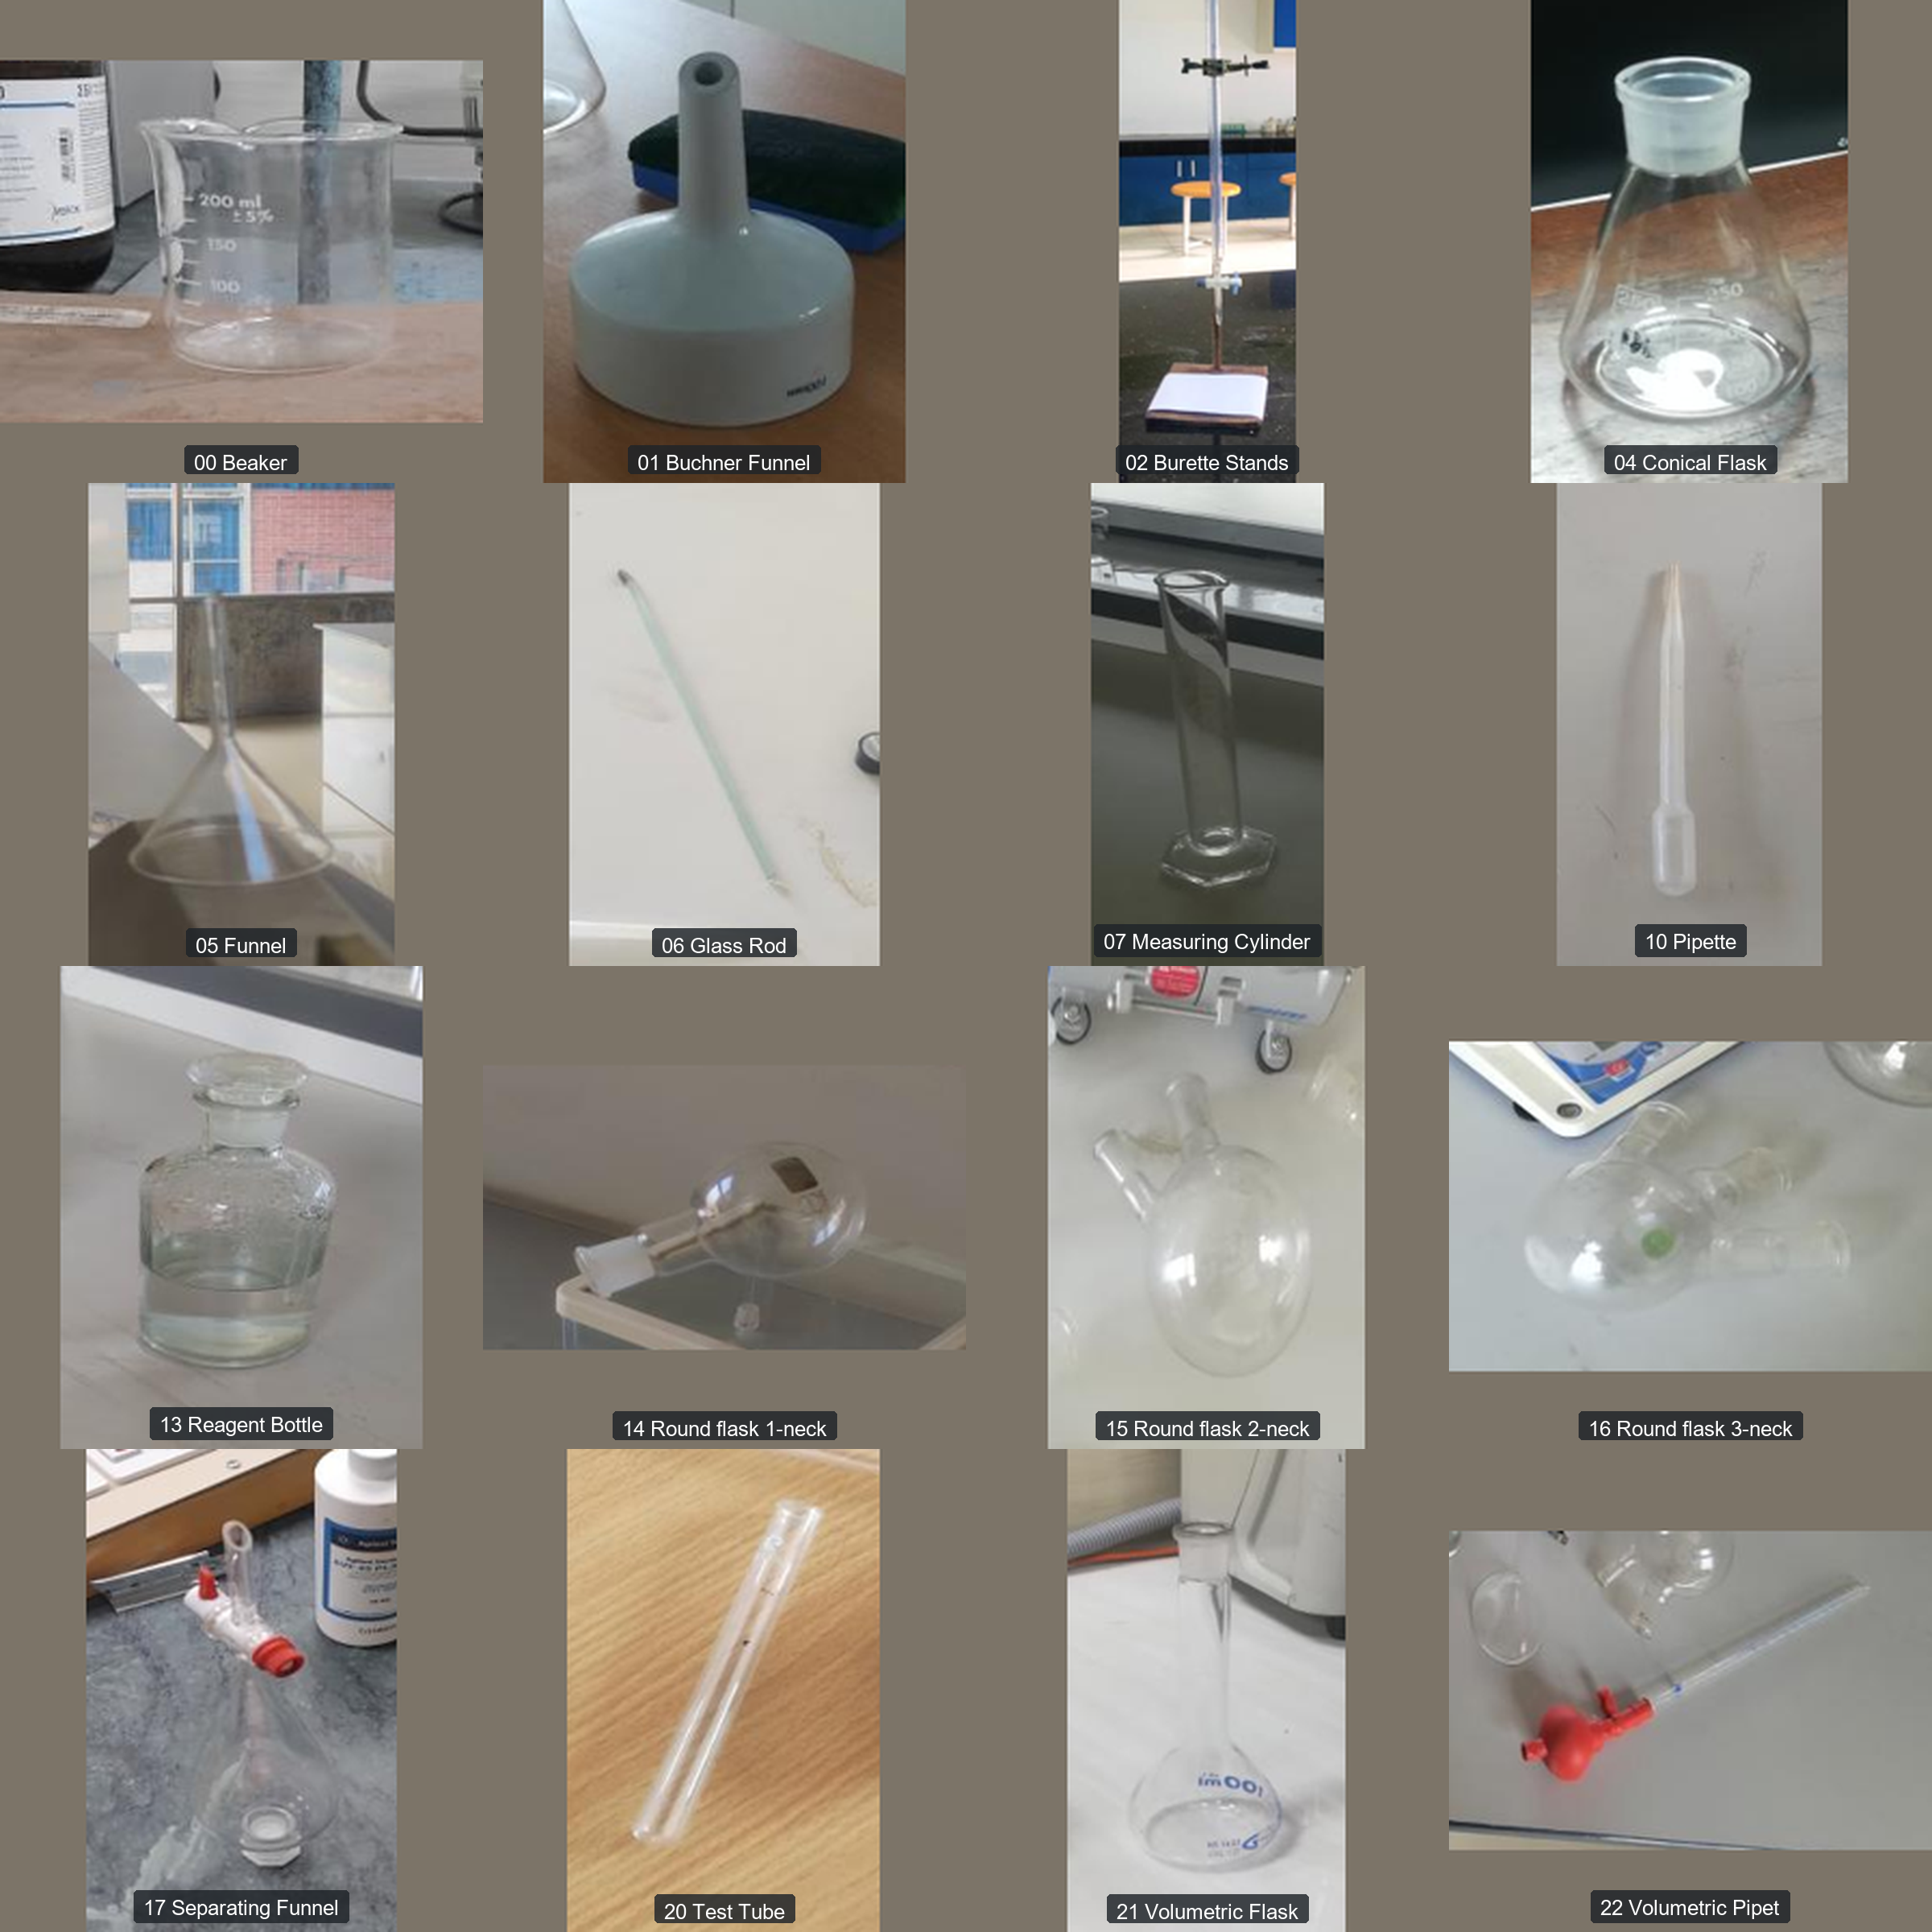
\includegraphics[width=\textwidth]{figures/tfg_dataset_classifier_crops_square.png}
        \caption{}
        \label{fig:crops}
    \end{subfigure}

    \caption{En la figura a) vemos ejemplos de cajas obtenidas a partir de las anotaciones YOLO. En la figura b) vemos ejemplos de los recortes utilizados como entrada del clasificador. El color gris que se ven entre las imágenes es el color de relleno cercano a la media de \textit{ImageNet}. Las imágenes en b) son los recortes tal y como las va a ver el modelo.}
    \label{fig:dataset_crops_YOLO}
\end{figure}

Una vez preparado el dataset, se lanzó el primer experimento serio con ChemEq25:

\begin{figure}[H]
    \centering
    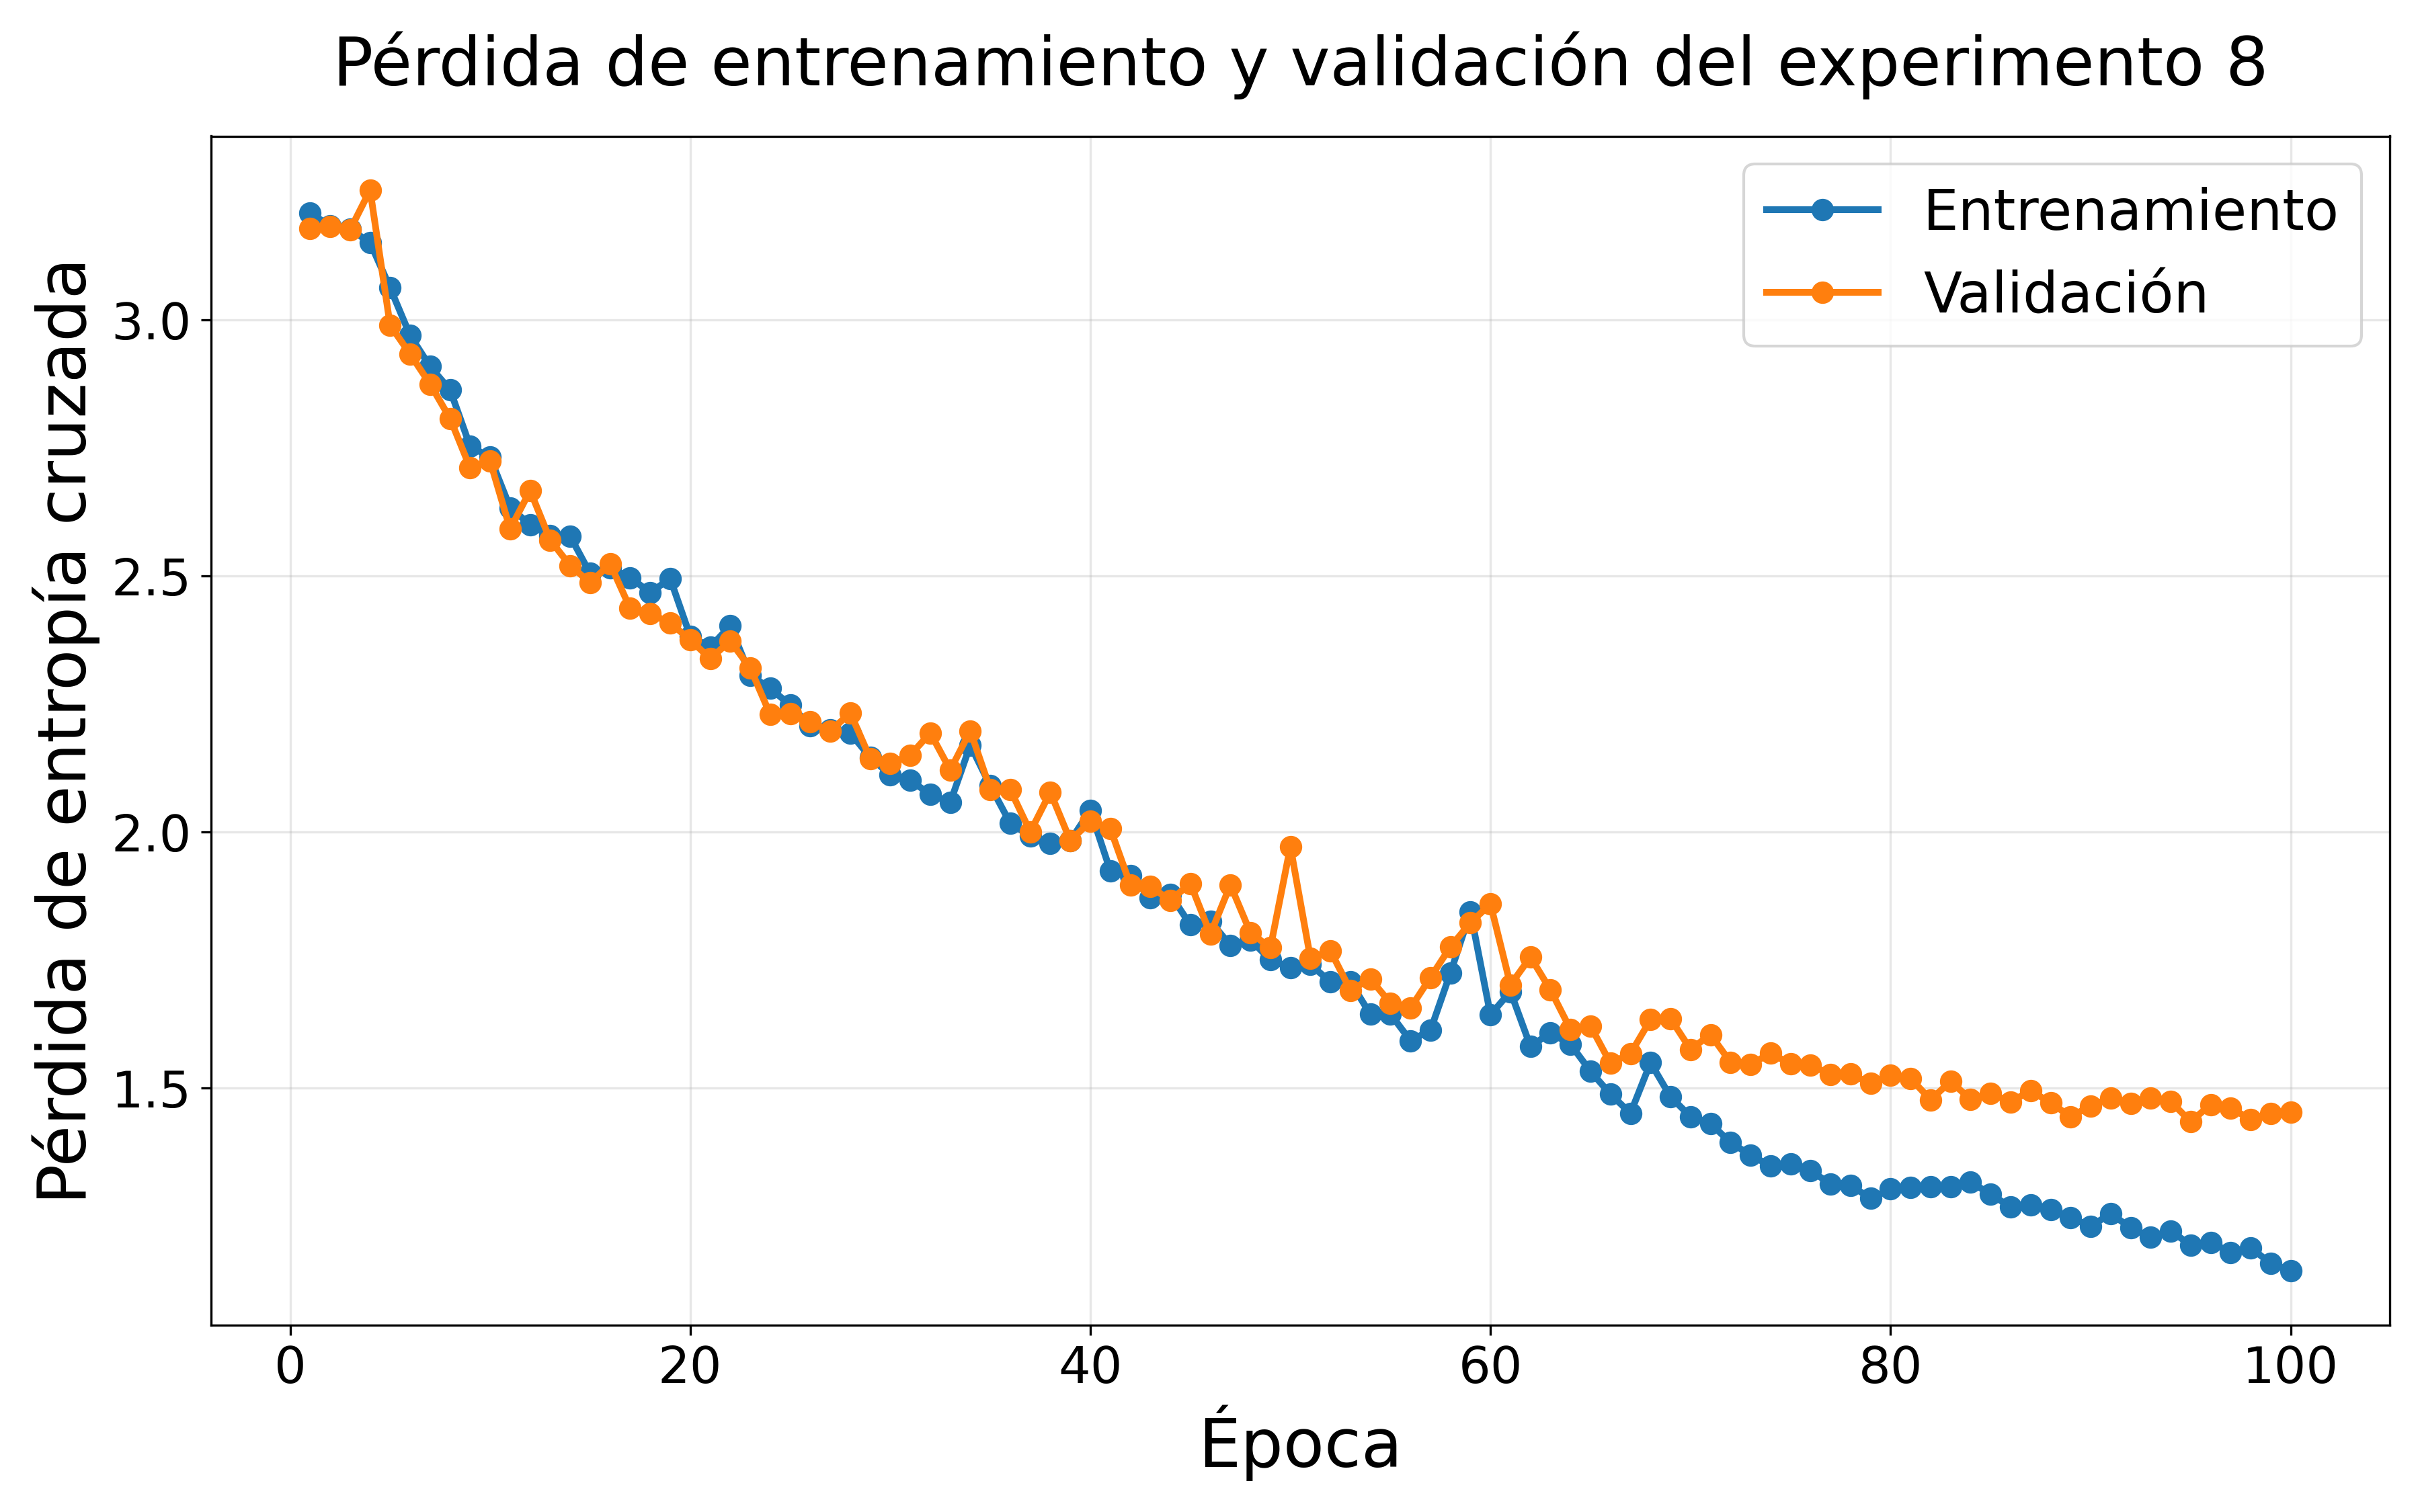
\includegraphics[width=0.55\linewidth]{figures/Experiments_logs/loss_curve_05-05-0953.png}
    \caption{Primer experimento con ChemEq25.}
    \label{fig:loss_curve_05-05-0953}
\end{figure}

\begin{table}[H]
\centering
\small
\begin{tabular}{lccccc}
\toprule
\textbf{Experimento} & \textbf{LR} & \textbf{Acc. eval} & \textbf{Top-5} & \textbf{Eval loss} & \textbf{Acc. final} \\
\midrule
\texttt{8} & 0,0005 & 57,00\% & 86,22\% & 1,4343 & 56,86\% \\
\bottomrule
\end{tabular}
\caption{Primer resultado sobre ChemEq25.}
\label{tab:chemeq_primer_run}
\end{table}

El salto respecto a Flowers102 fue muy grande. La precisión pasó de 33,96\% en Flowers a 57,00\% en ChemEq25, y el top-5 alcanzó 86,22\%. Esto confirmó la hipótesis 3. El problema de Flowers102 no era solo la arquitectura, sino también la dificultad de separar 102 clases de flores muy parecidas. Con 25 clases de material de laboratorio, el modelo empezó a mostrar mucha más capacidad.

\subsection{Efecto del learning rate}

El siguiente cambio fue reducir el \textit{learning rate} de 0,0005 a 0,00025. El \textit{learning rate} es el tamaño del paso que da el optimizador al actualizar los parámetros. Si es demasiado alto, el modelo puede moverse de forma brusca por el espacio de parámetros y no estabilizarse bien. Si es demasiado bajo, el entrenamiento puede avanzar muy lento.

\begin{figure}[H]
    \centering

    \begin{subfigure}{0.45\textwidth}
        \centering
        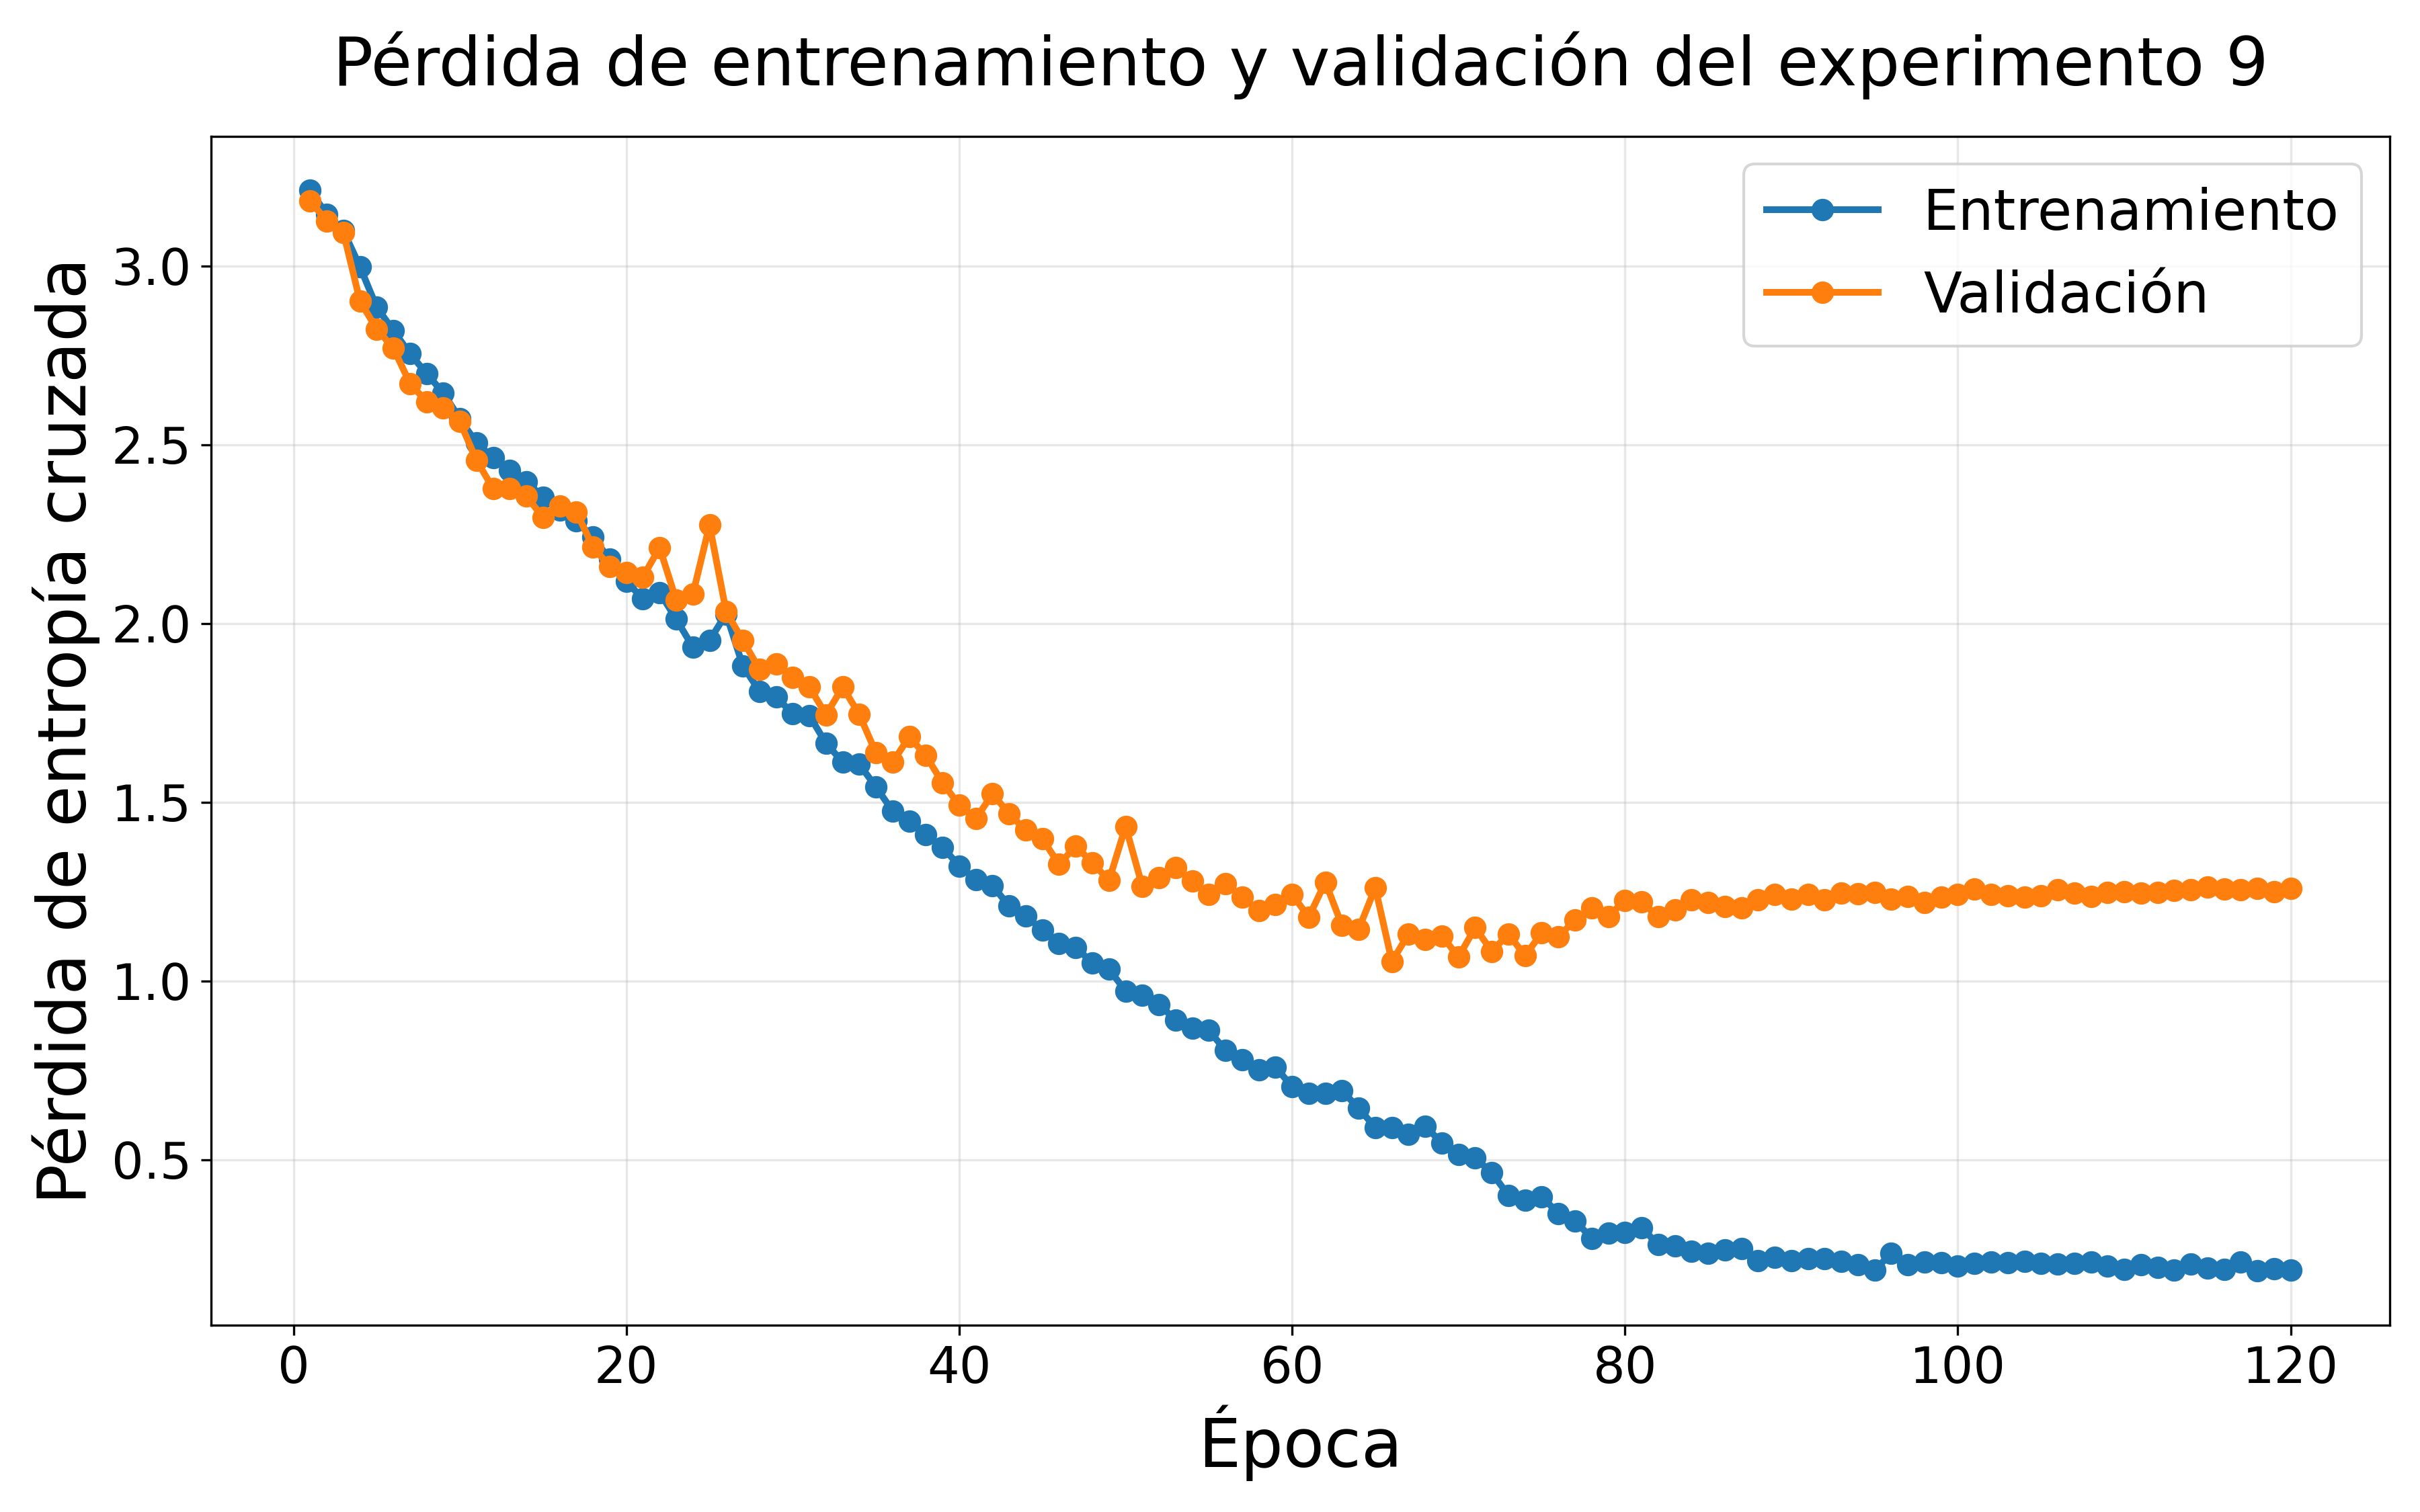
\includegraphics[width=\textwidth]{figures/Experiments_logs/loss_curve_05-05-1119.png}
        \caption{}
        \label{fig:loss_curve_05-05-1119}
    \end{subfigure}
    \hfill
    \begin{subfigure}{0.45\textwidth}
        \centering
        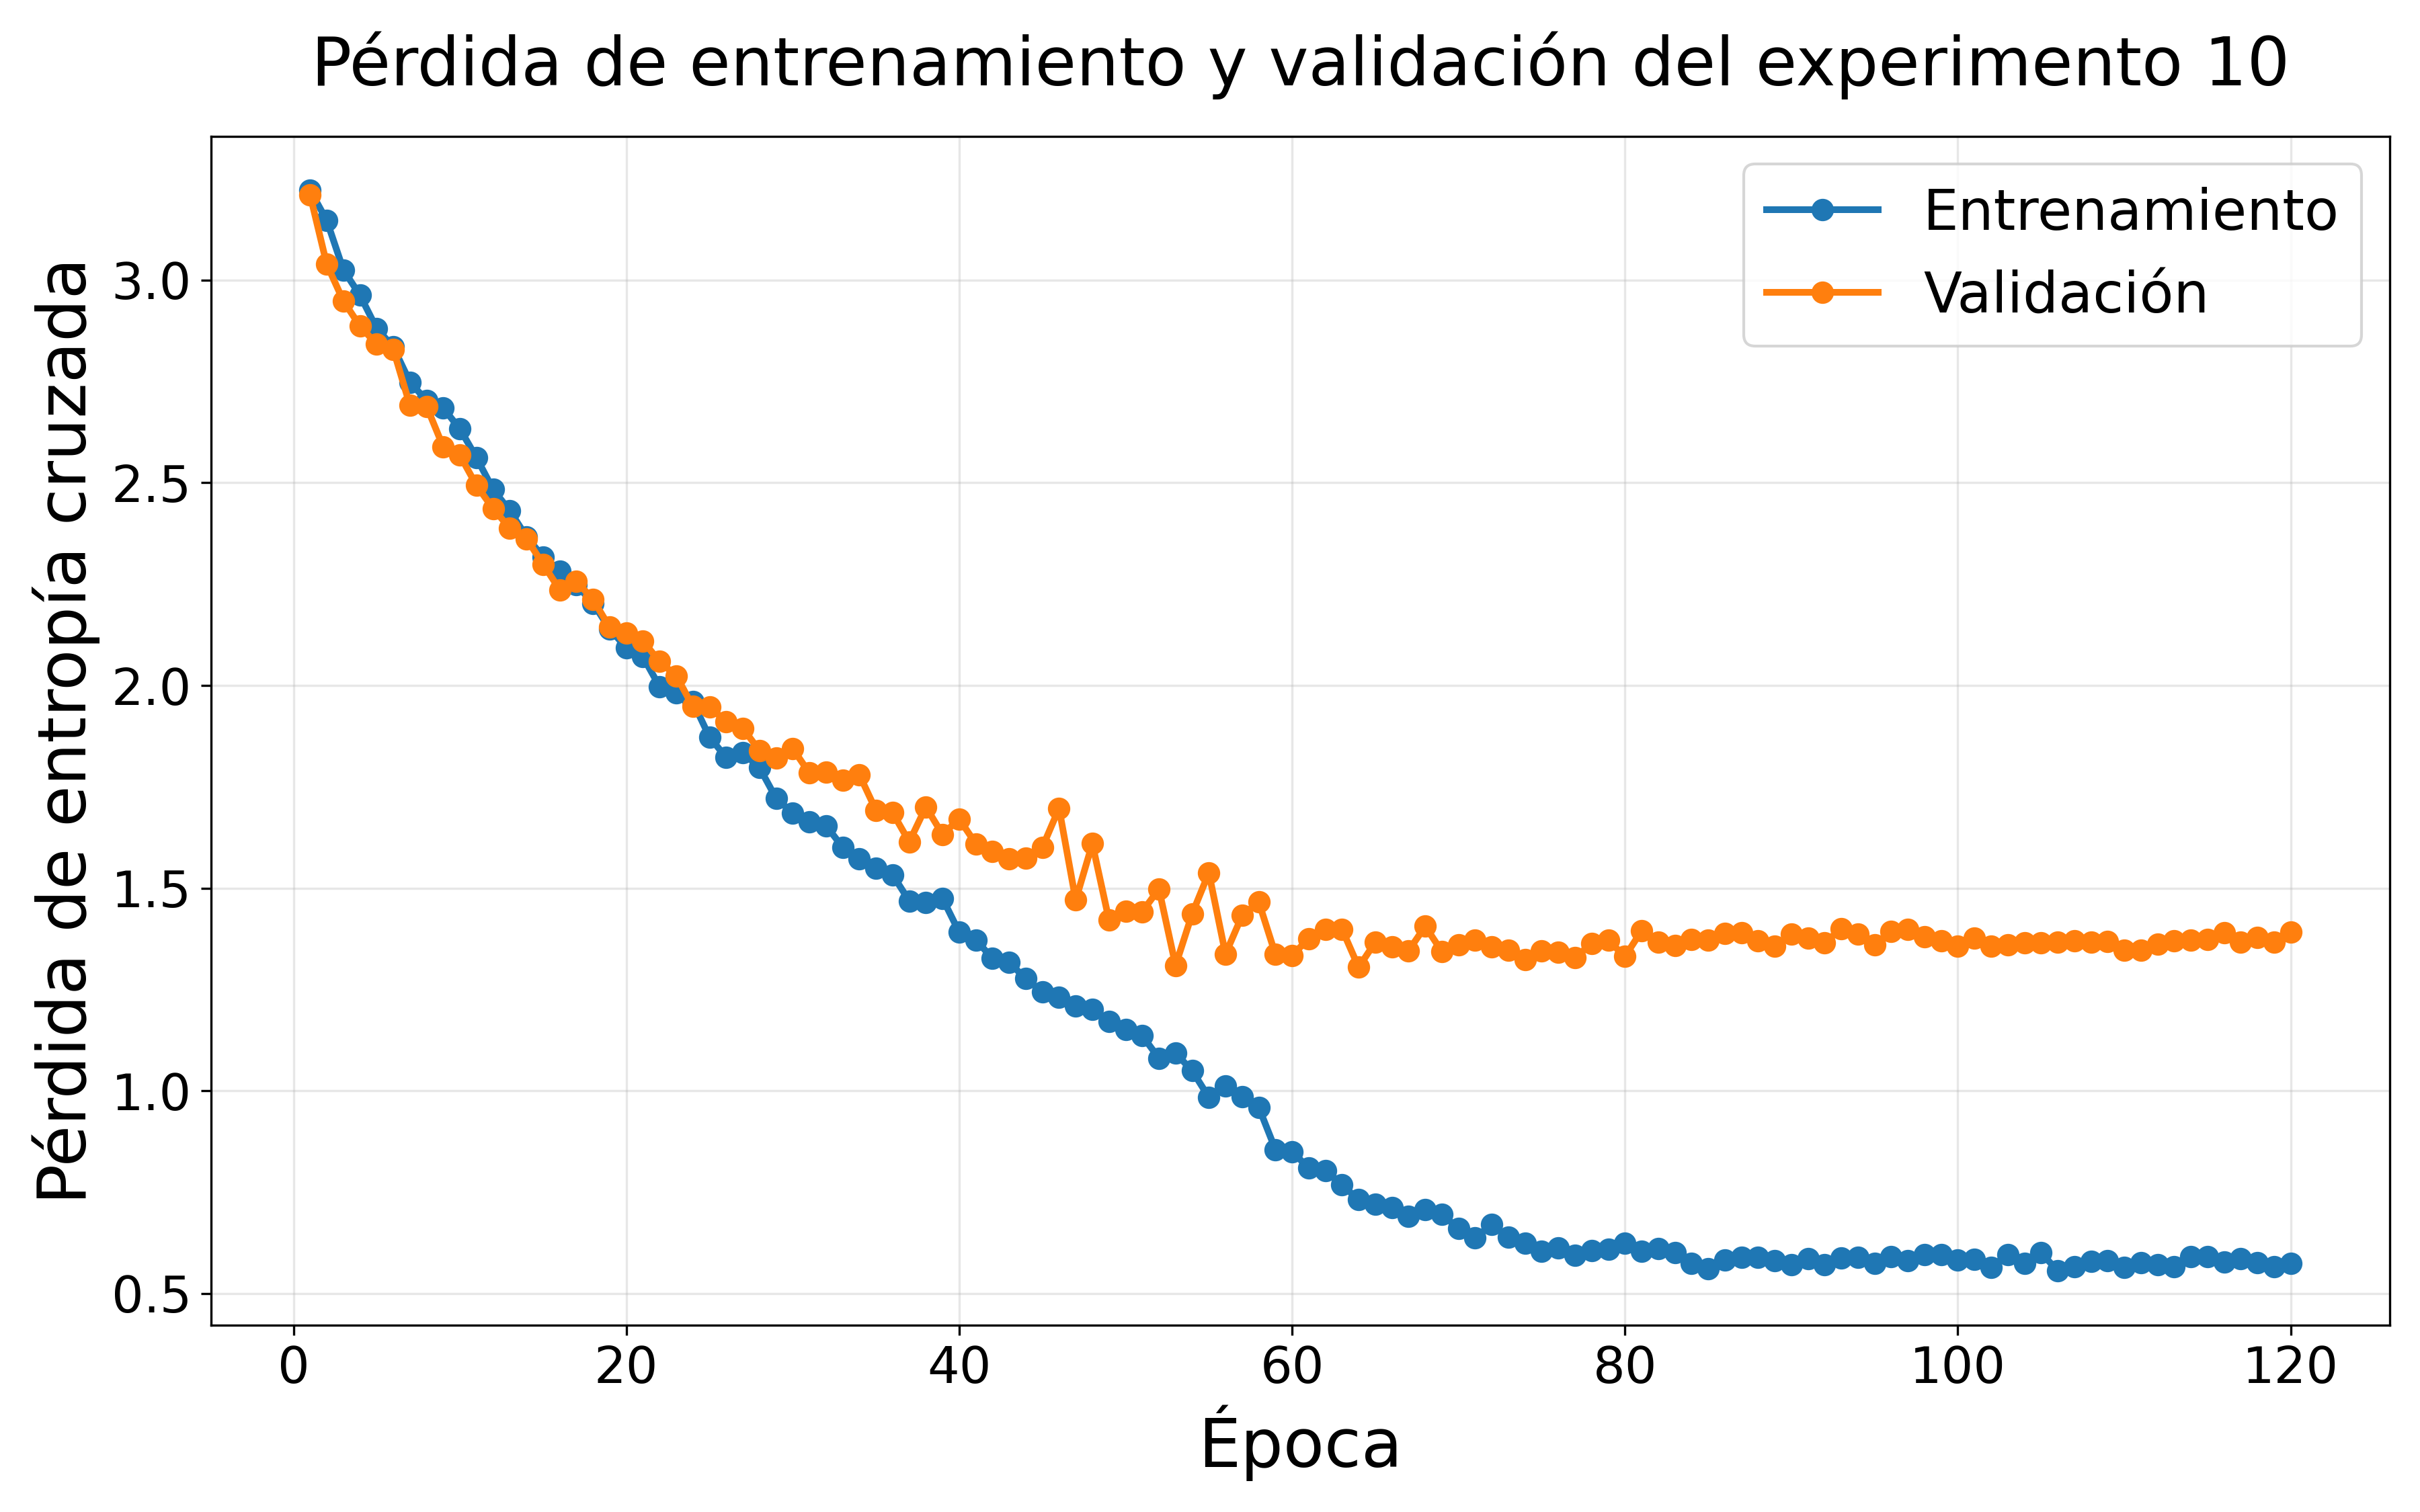
\includegraphics[width=\textwidth]{figures/Experiments_logs/loss_curve_05-05-1145.png}
        \caption{}
        \label{fig:loss_curve_05-05-1145}
    \end{subfigure}

    \caption{Mismo experimento que \figref{fig:loss_curve_05-05-0953}, pero con \textit{learning rate} menor.}
    \label{fig:loss_curve_05-05-1119-1145}
\end{figure}

\begin{table}[H]
\centering
\scriptsize
\begin{tabular}{lcccccc}
\toprule
\textbf{Experimento} & \textbf{Cambio} & \textbf{Acc.} & \textbf{Top-5} & \textbf{Loss} & \textbf{Train final} & \textbf{Eval final} \\
\midrule
\texttt{8} & LR 0,0005 & 57,00\% & 86,22\% & 1,4343 & 64,80\% & 56,86\% \\
\texttt{9} & LR 0,00025 & 75,23\% & 93,90\% & 1,0539 & 94,78\% & 74,66\% \\
\texttt{10} & MLP head & 70,57\% & 94,33\% & 1,3047 & 80,34\% & 69,56\% \\
\bottomrule
\end{tabular}
\caption{Comparación de los primeros ajustes sobre ChemEq25.}
\label{tab:chemeq_lr_head}
\end{table}

La bajada del \textit{learning rate} produjo una mejora muy fuerte: de 57,00\% a 75,23\%. Esto no significa que el modelo empezara desde un punto distinto, porque la \textit{seed} era la misma. Lo que cambió fue la trayectoria de optimización. Con pasos más pequeños, el modelo encontró una zona mucho mejor.

También se probó una cabeza MLP en vez de una cabeza lineal. La motivación era que el top-5 era alto, así que quizá la representación final contenía información suficiente, pero faltaba una separación más fina entre clases. Sin embargo, la MLP no mejoró el resultado, se quedó en 70,57\%. Por eso se mantuvo la cabeza lineal como opción principal.

En el experiemento con \textit{learning rate} 0,00025 apareció otro patrón interesante. La mejor \textit{eval loss} se alcanzó en la época 66, pero la mejor precisión llegó en la época 104. Esto indica que el modelo acertaba más ejemplos, pero cuando fallaba podía hacerlo con más confianza. Esa lectura motivó los siguientes cambios, \textit{warmup}, regularización y \textit{label smoothing}.

\section{Ajustes de entrenamiento y regularización}

A partir de este punto hubo muchos experimentos. Por cada experimento que se hacía, se iban atacando los problemas observados. Optimización inestable, sobreconfianza, clases parecidas y sensibilidad a la seed.

\begin{figure}[htbp]
    \centering

    \begin{subfigure}{0.45\textwidth}
        \centering
        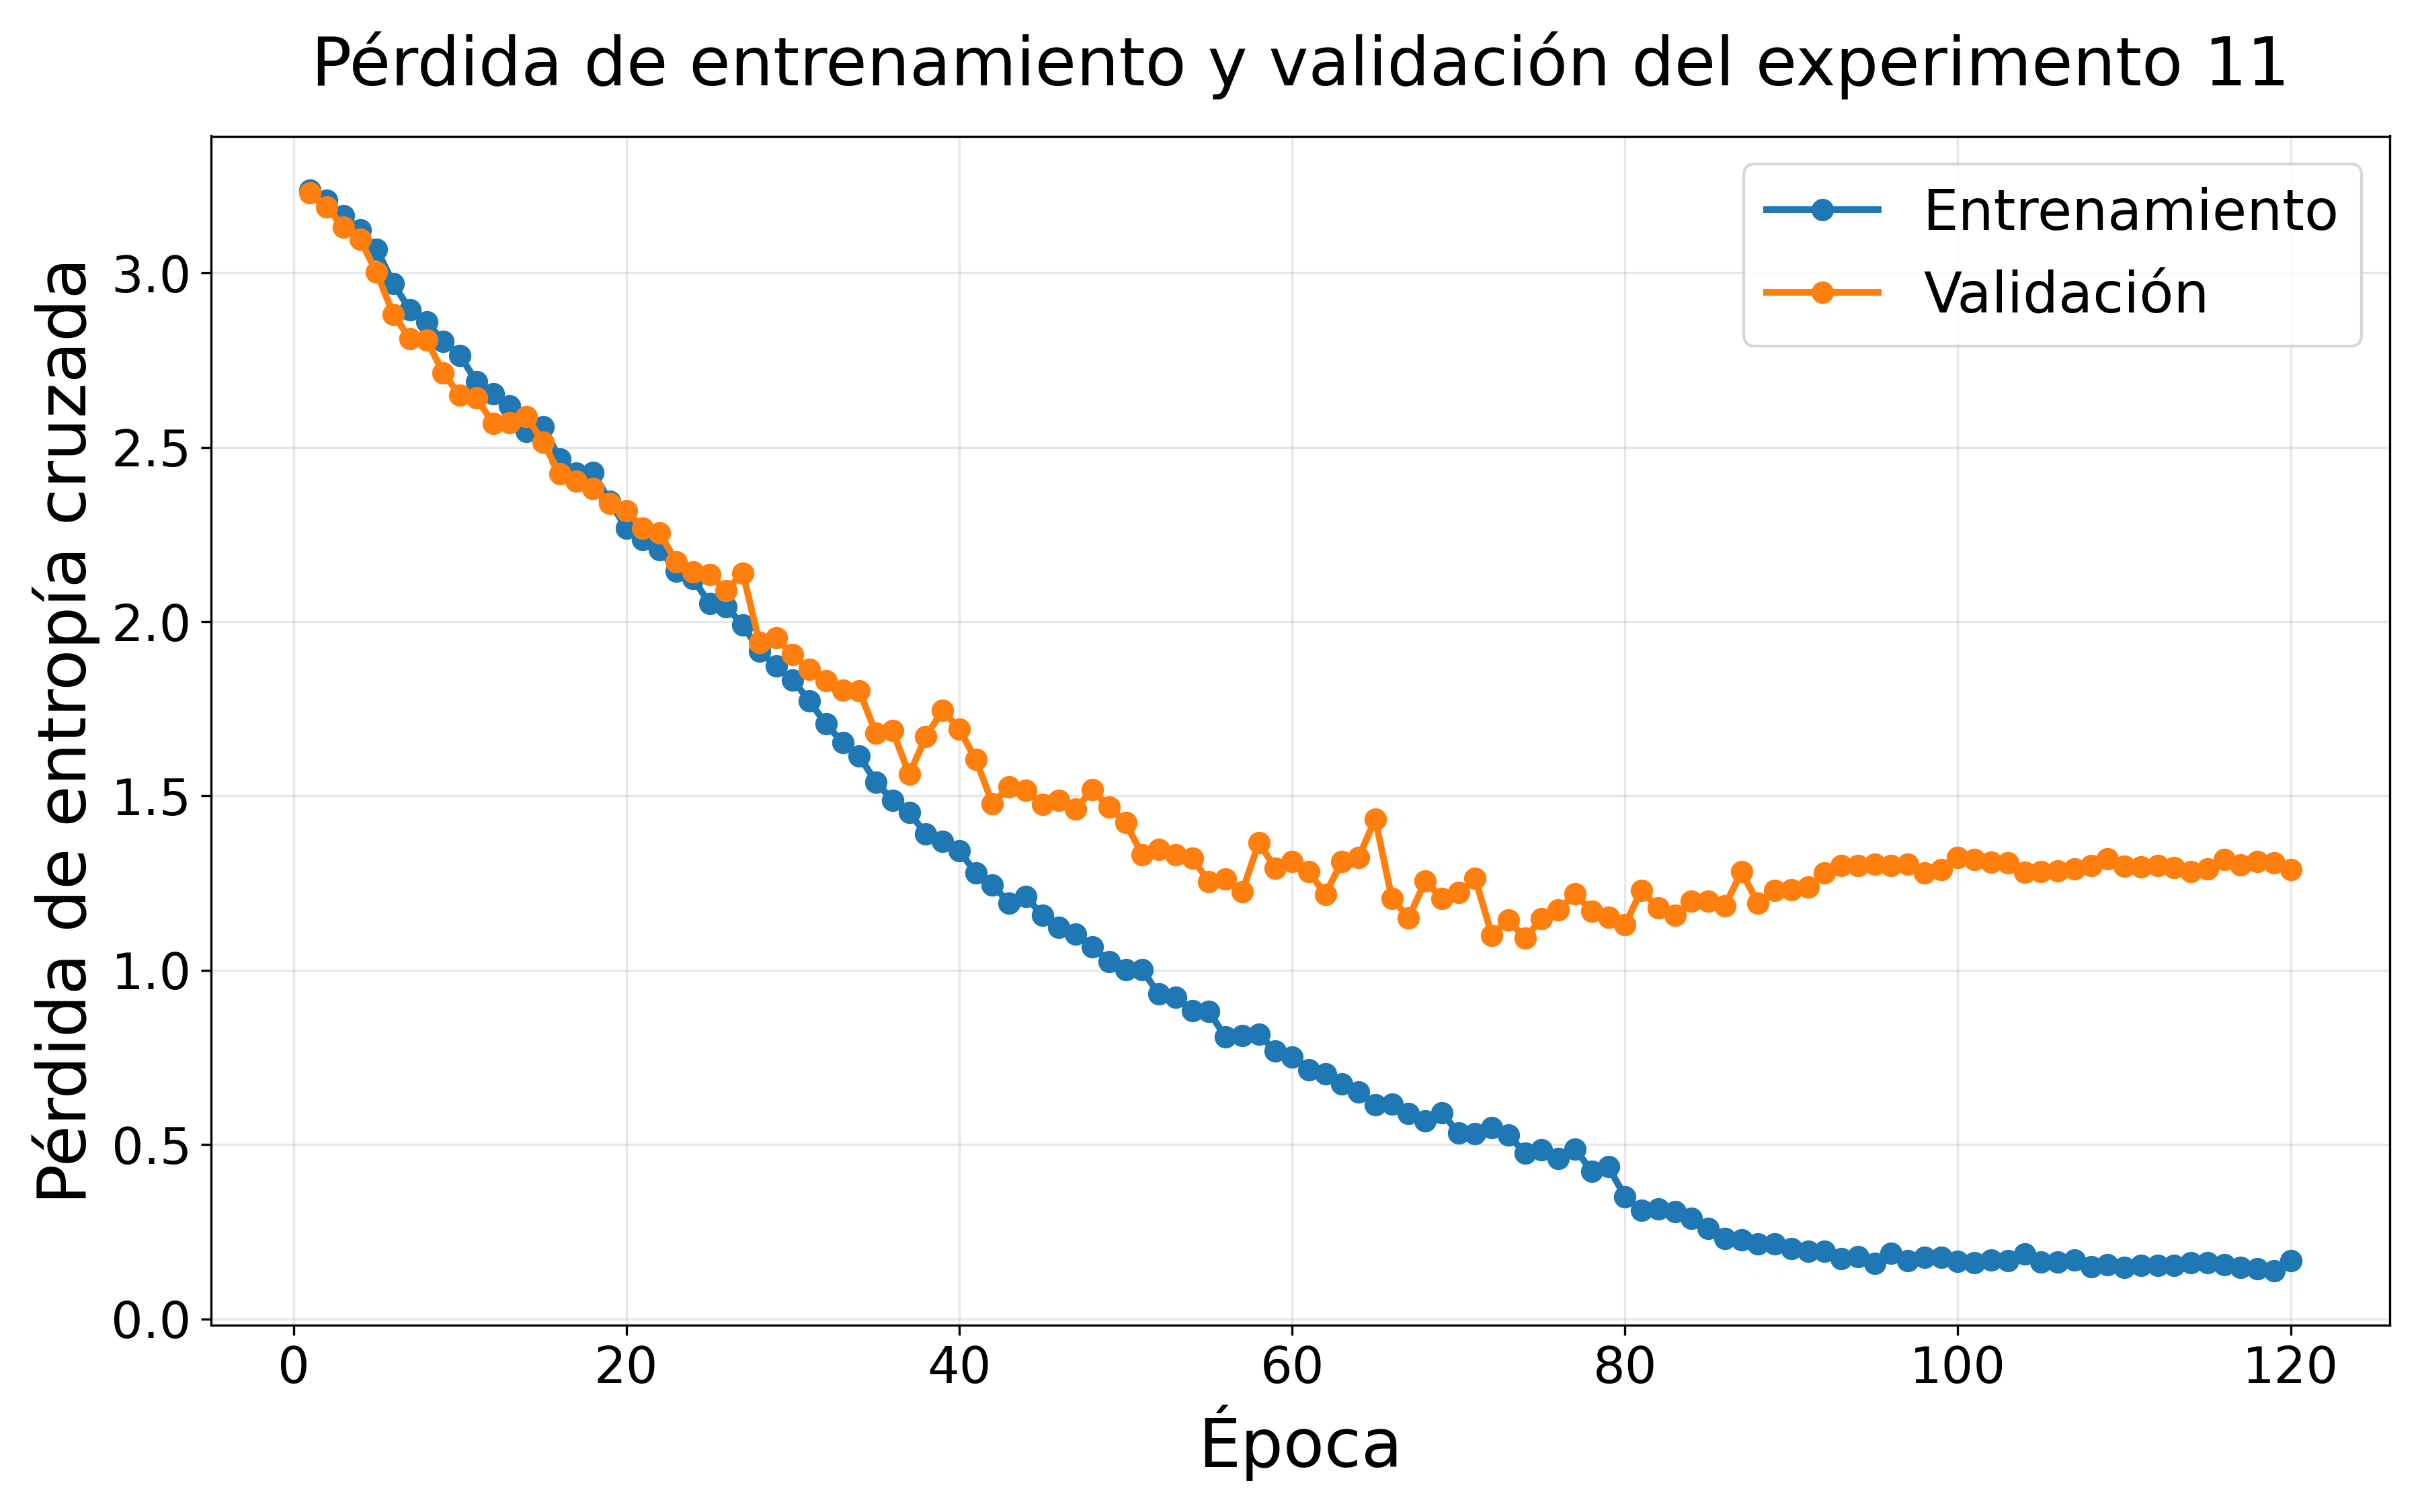
\includegraphics[width=\textwidth]{figures/Experiments_logs/loss_curve_05-07-0857.png}
        \caption{}
        \label{fig:loss_curve_05-07-0857}
    \end{subfigure}
    \hfill
    \begin{subfigure}{0.45\textwidth}
        \centering
        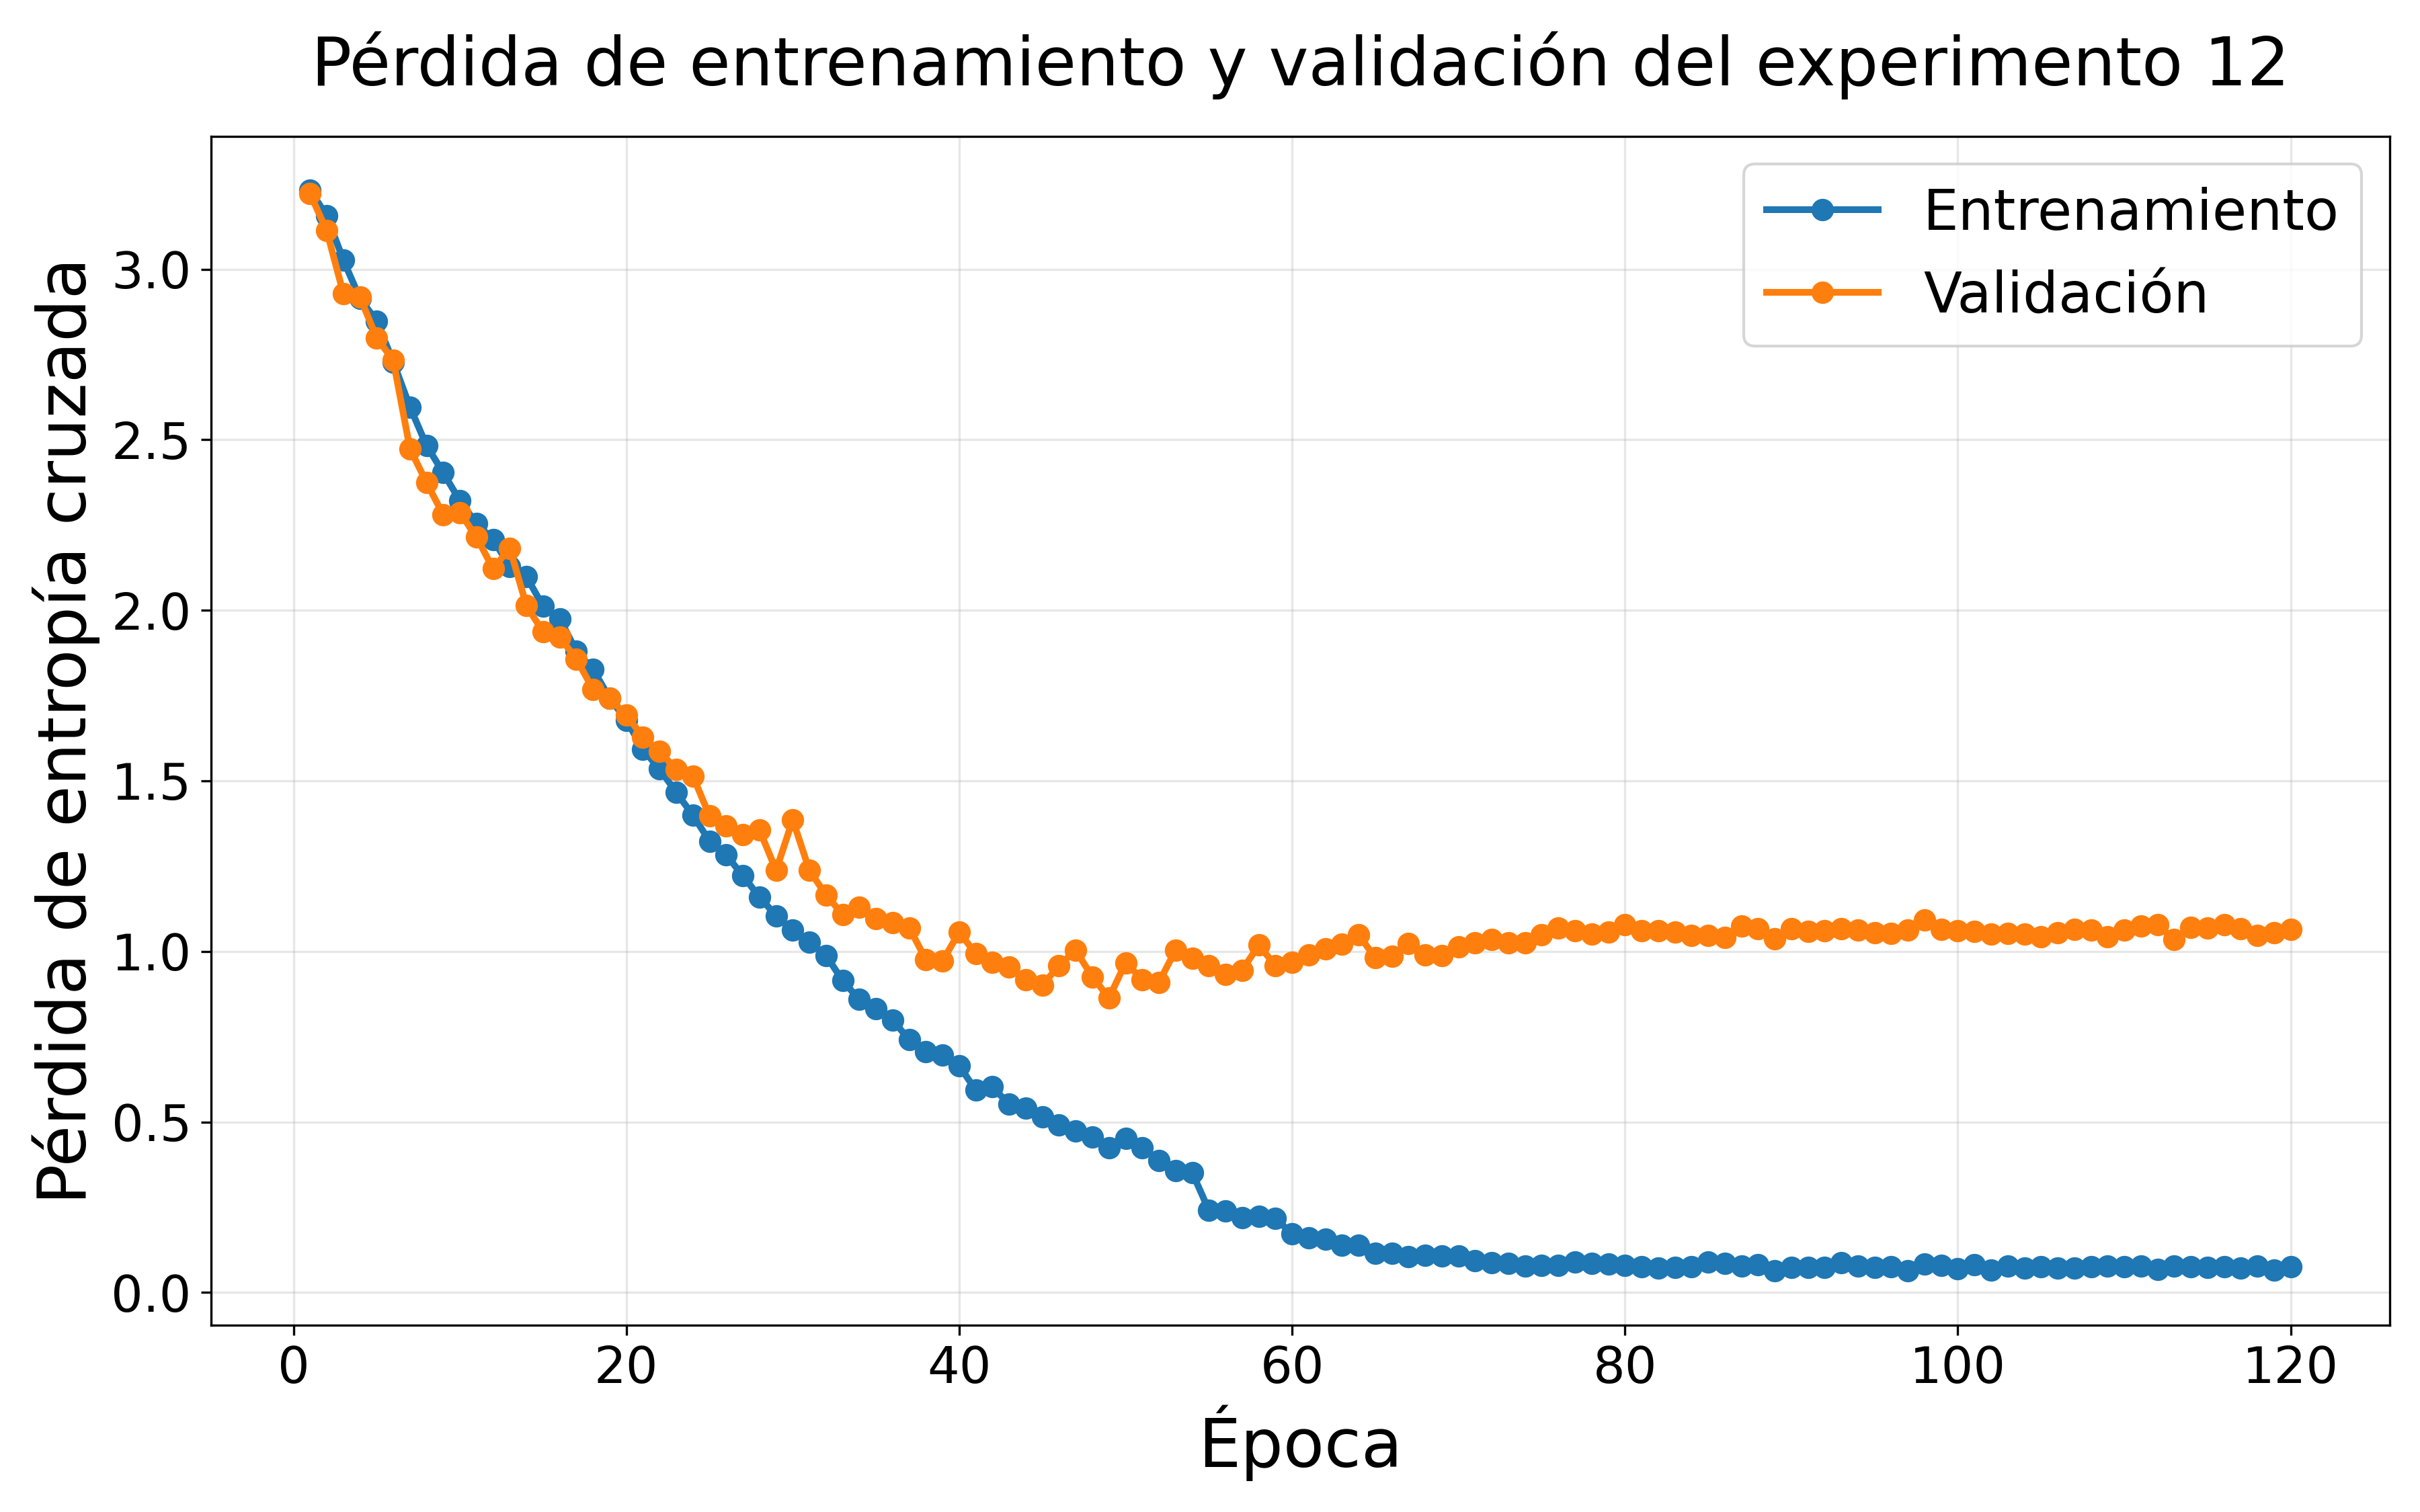
\includegraphics[width=\textwidth]{figures/Experiments_logs/loss_curve_05-07-1304.png}
        \caption{}
        \label{fig:loss_curve_05-07-1304}
    \end{subfigure}

    \vspace{0.4cm}

    \begin{subfigure}{0.45\textwidth}
        \centering
        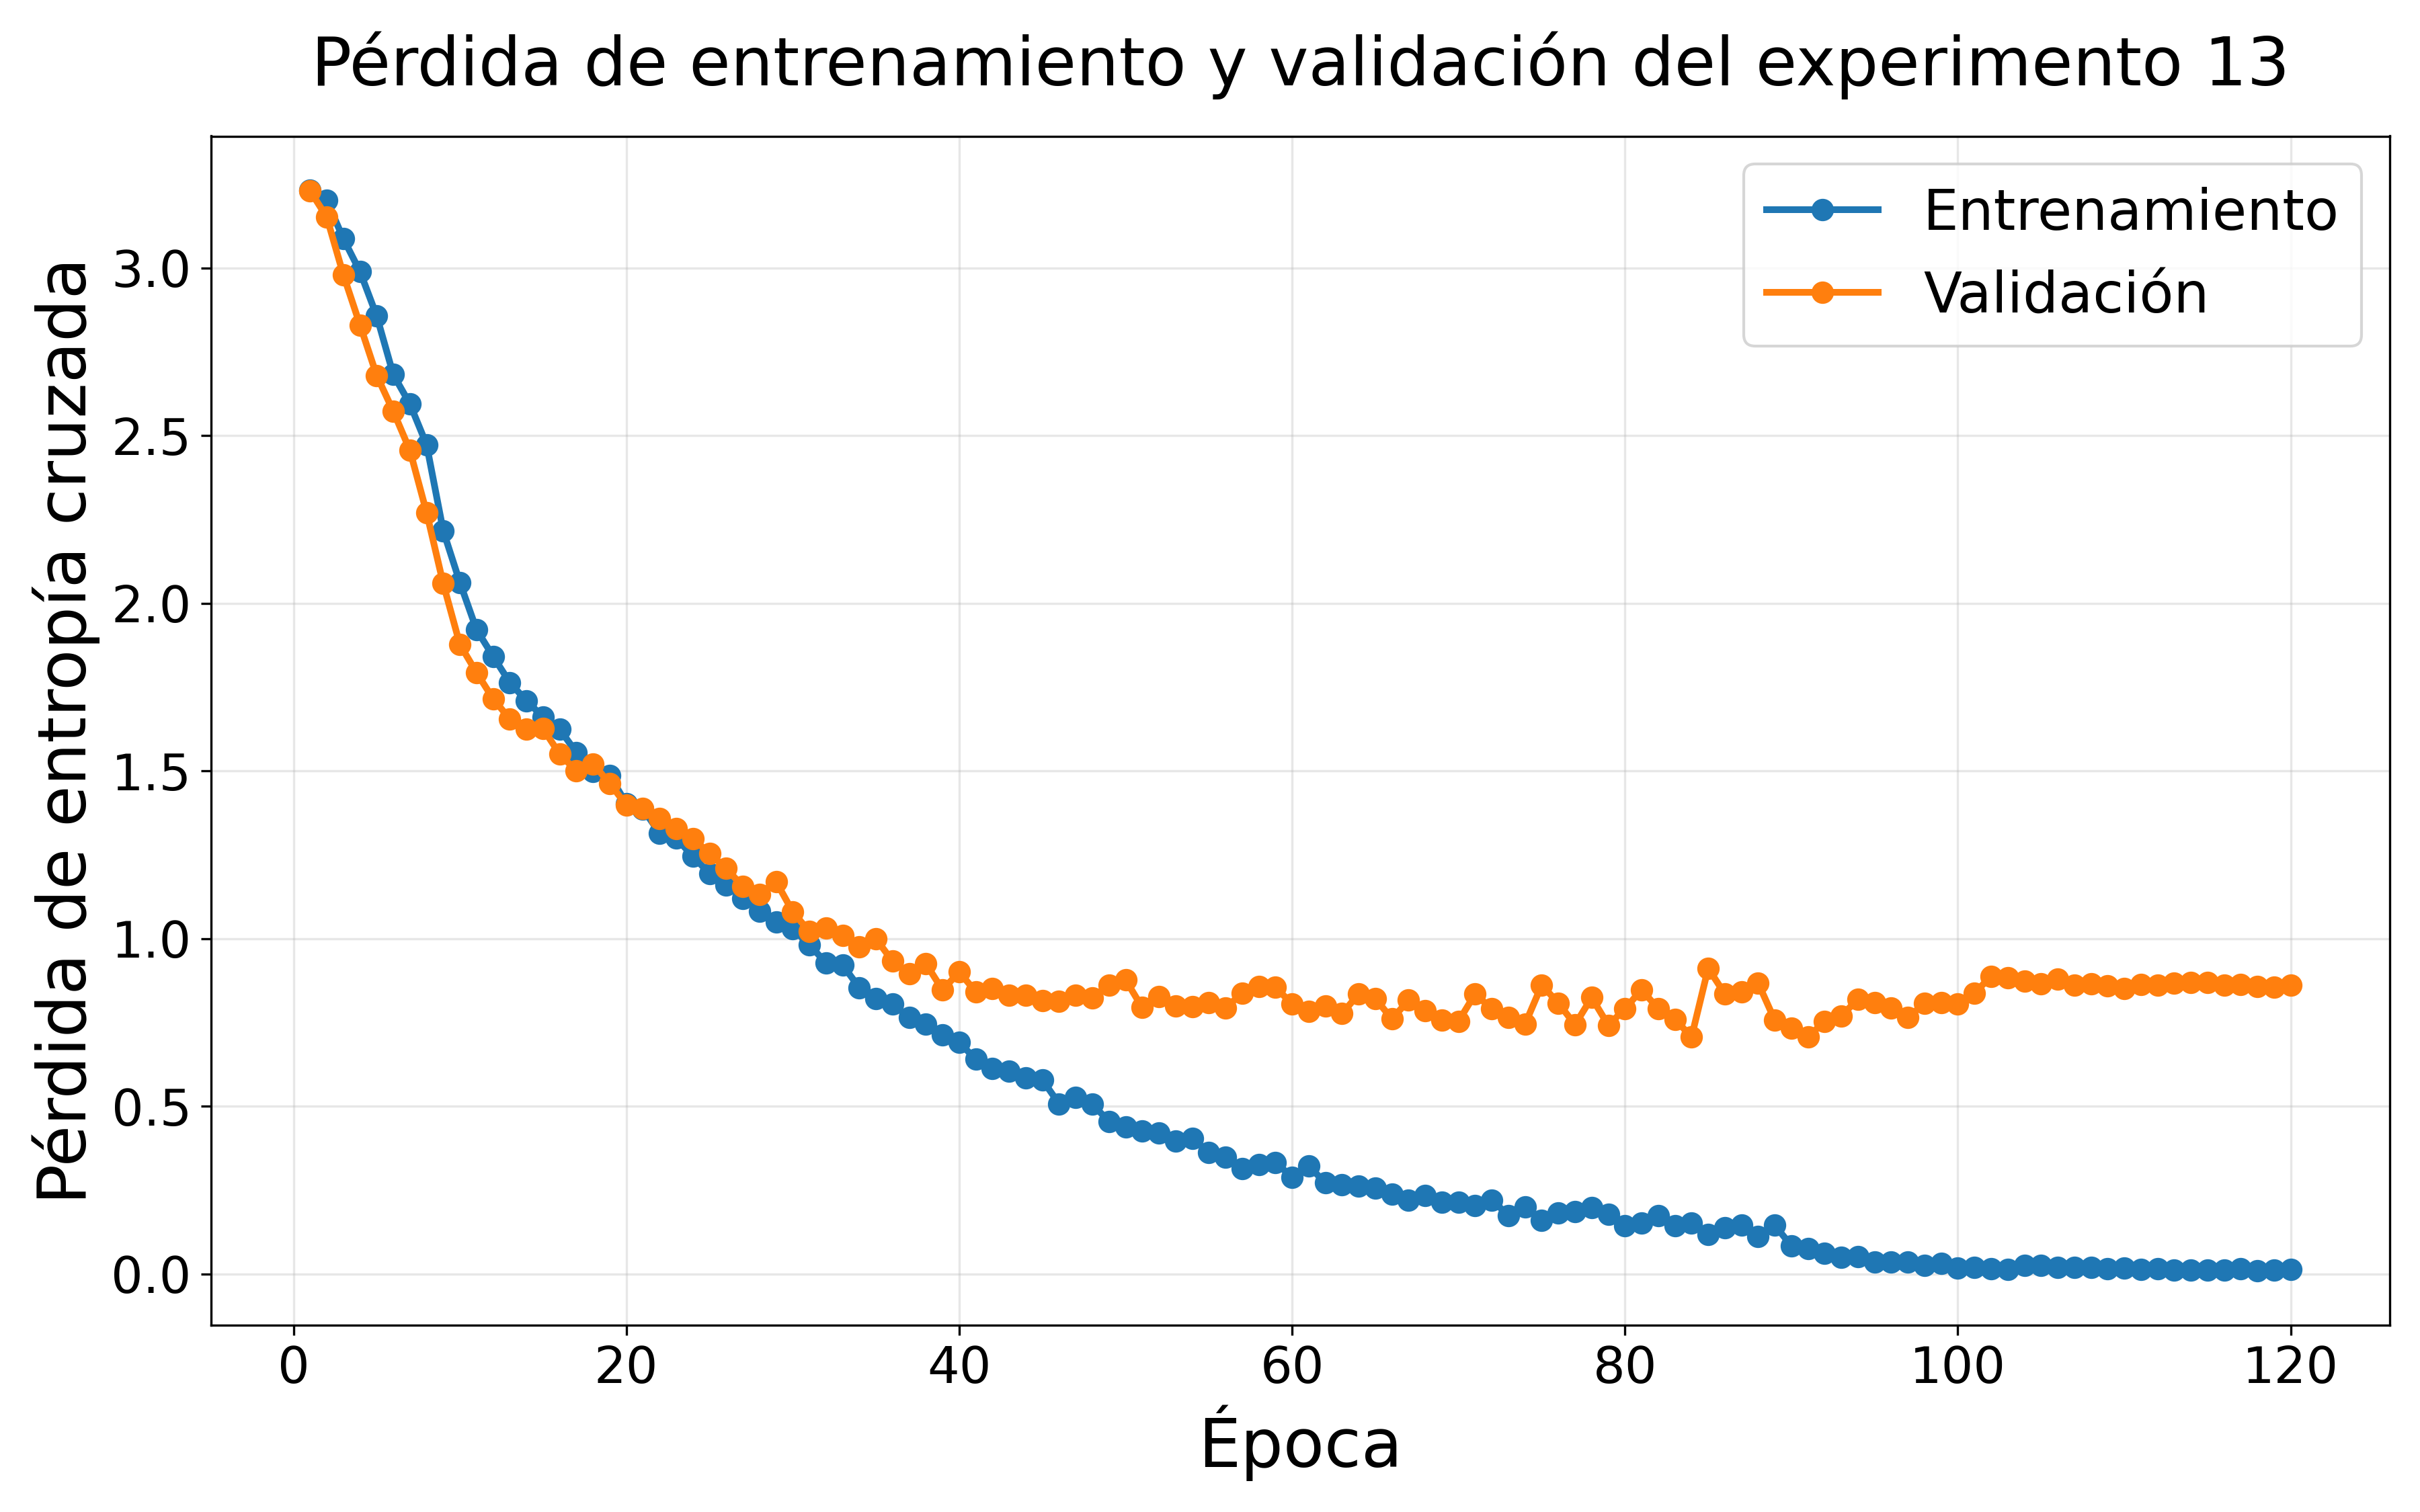
\includegraphics[width=\textwidth]{figures/Experiments_logs/loss_curve_05-08-1400.png}
        \caption{}
        \label{fig:loss_curve_05-08-1400}
    \end{subfigure}
    \hfill
    \begin{subfigure}{0.45\textwidth}
        \centering
        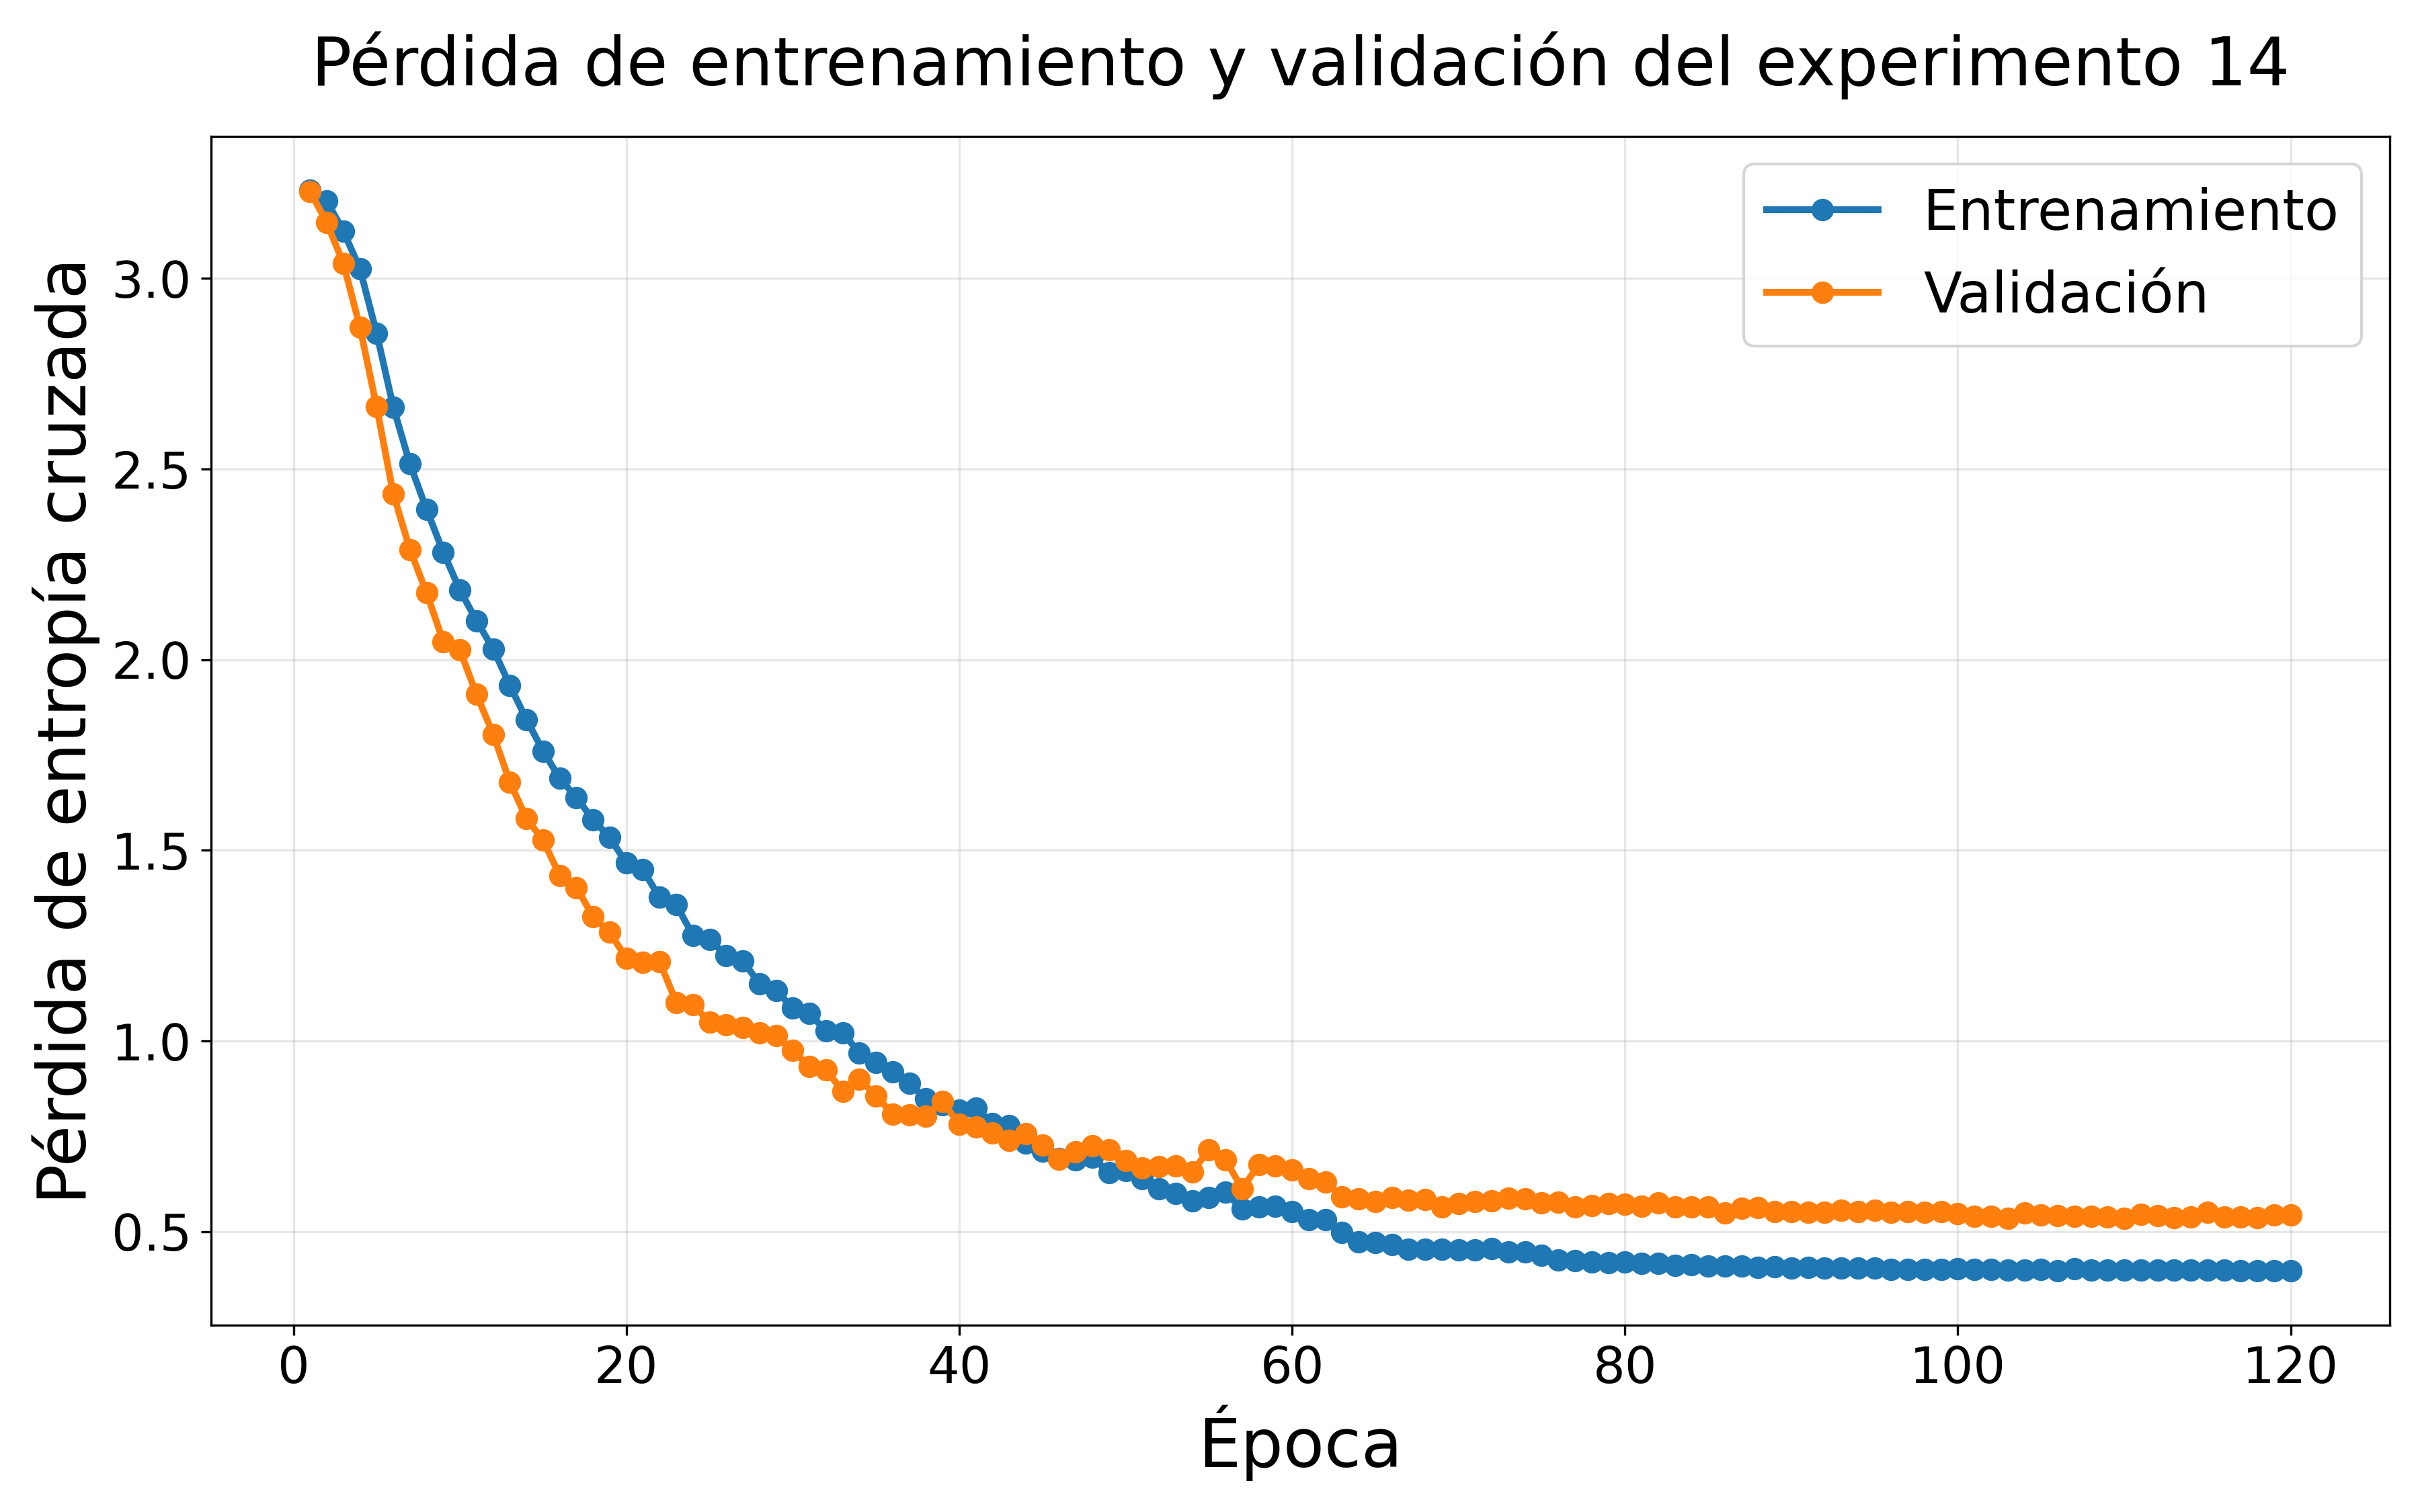
\includegraphics[width=\textwidth]{figures/Experiments_logs/loss_curve_05-11-0958.png}
        \caption{}
        \label{fig:loss_curve_05-11-0958}
    \end{subfigure}

     \vspace{0.4cm}

    \begin{subfigure}{0.45\textwidth}
        \centering
        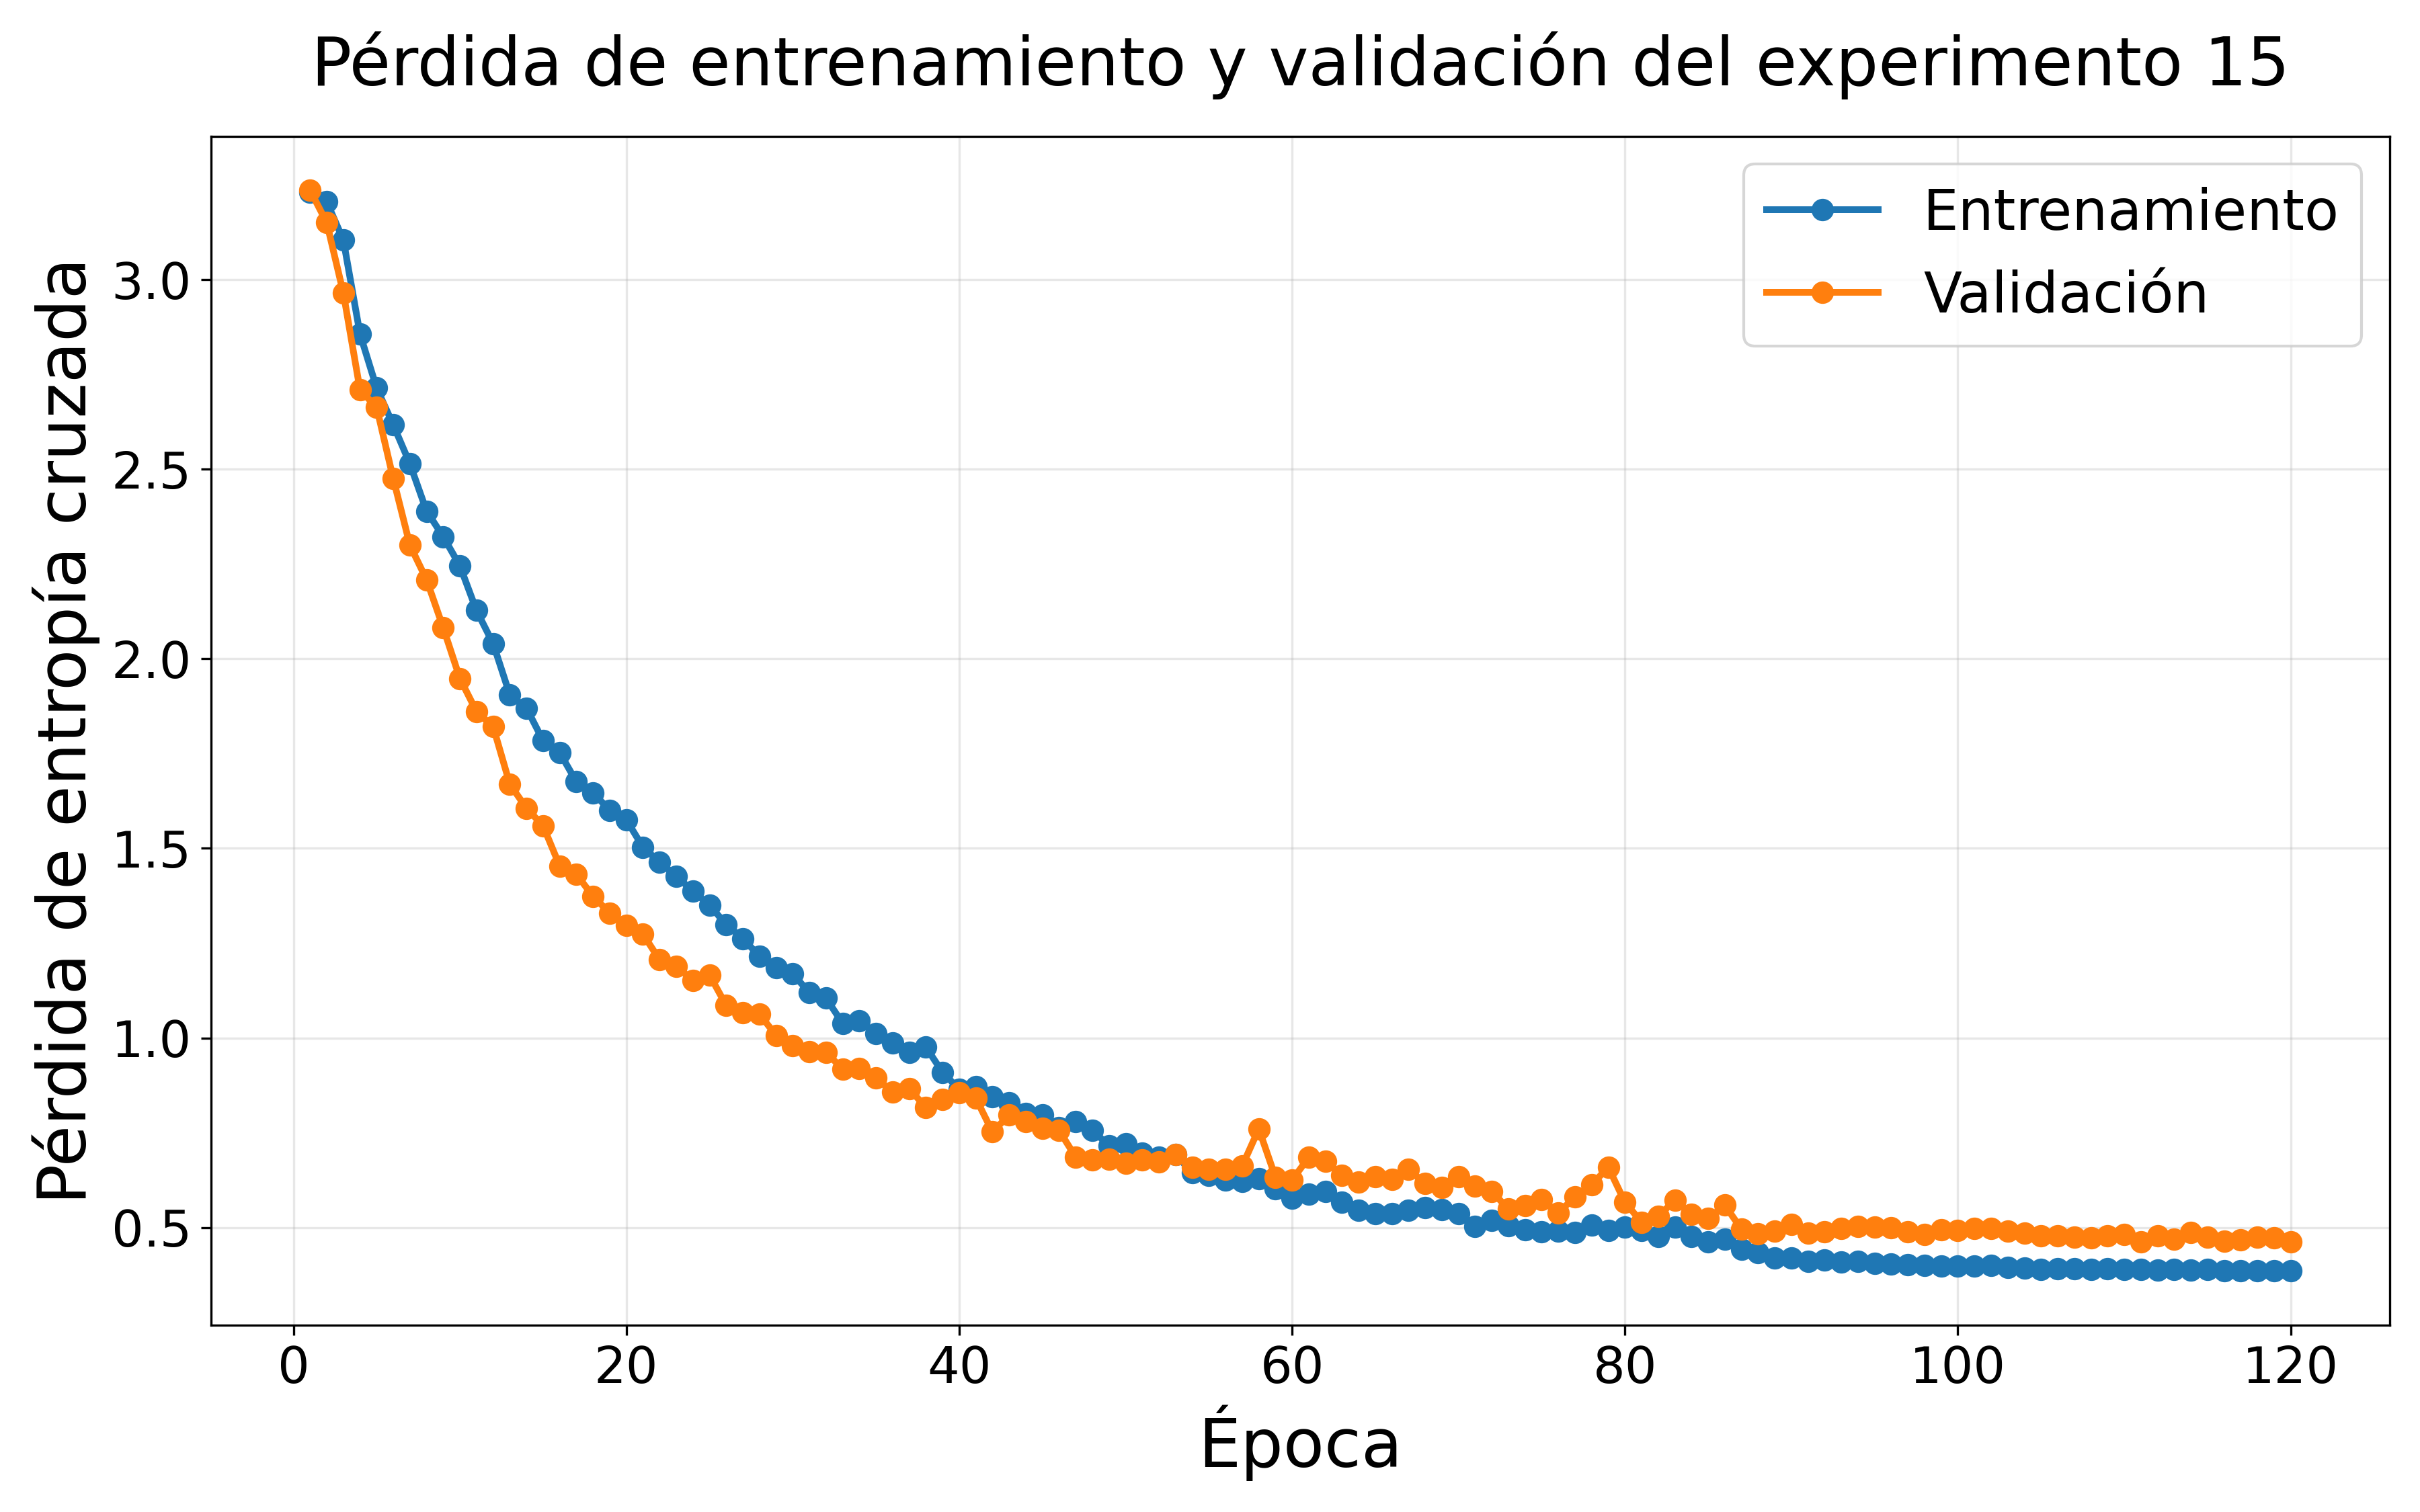
\includegraphics[width=\textwidth]{figures/Experiments_logs/loss_curve_05-11-1101.png}
        \caption{}
        \label{fig:loss_curve_05-11-1101}
    \end{subfigure}

    \caption{Distintos experimentos a los que se le fueron aplicando pequeñas mejoras detalladas en \tabref{tab:ajustes_entrenamiento}. Se puede ver como las curvas de perdida van mejorando con cada experimento.}
    \label{fig:loss_curve-07-11}
\end{figure}

\begin{table}[H]
\centering
\small
\begin{tabularx}{\textwidth}{lXcccc}
\toprule
\textbf{Experimento} & \textbf{Cambio principal} & \textbf{Mejor acc.} & \textbf{Top-5} & \textbf{Mejor loss} & \textbf{Acc. final} \\
\midrule
\texttt{11} & Warmup con configuración 8/8 & 78,46\% & 94,62\% & 1,0915 & 78,03\% \\
\texttt{12} & Subida a dimensión 12/12 & 81,55\% & 95,41\% & 0,8637 & 80,33\% \\
\texttt{13} & Warmup coseno, preservación de aspecto y $L_2$ suave & 86,86\% & 97,77\% & 0,7065 & 86,43\% \\
\texttt{14} & Label smoothing 0,05, seed 42 & 87,08\% & 96,77\% & 0,5221 & 86,93\% \\
\texttt{15} & Repetición del experimento con label smoothing 0,05 & 88,94\% & 97,20\% & 0,4617 & 88,44\% \\
\bottomrule
\end{tabularx}
\caption{Evolución de los ajustes de entrenamiento antes del último cambio de \textit{data augmentation}.}
\label{tab:ajustes_entrenamiento}
\end{table}

El \textit{warmup} ayudó a que el entrenamiento no empezara de forma tan agresiva. Subir \texttt{local\_dim} y \texttt{bond\_dim} a 12 también mejoró bastante, porque la representación que entraba en la TTN y el vector interno de enlace tenían más capacidad.

Después, la combinación de warmup coseno mas la preservación de relación de aspecto de las imágenes recortadas y la implementación de un término de regularización $L_2$, llevó el modelo hasta 86,86\% de precisión. En este punto el modelo ya funcionaba bien, pero seguía habiendo sobreconfianza en los errores. Por eso se incorporó \textit{label smoothing}. Con \texttt{label\_smoothing=0.05} no solo mejoró ligeramente la precisión, sino que bajó de forma clara la pérdida de evaluación y la confianza media cuando el modelo se equivocaba.

\begin{figure}[htbp]
    \centering
    \captionsetup[subfigure]{skip=1pt}
    \captionsetup[figure]{font=footnotesize, skip=3pt}
    
    \begin{subfigure}{0.45\textwidth}
        \centering
        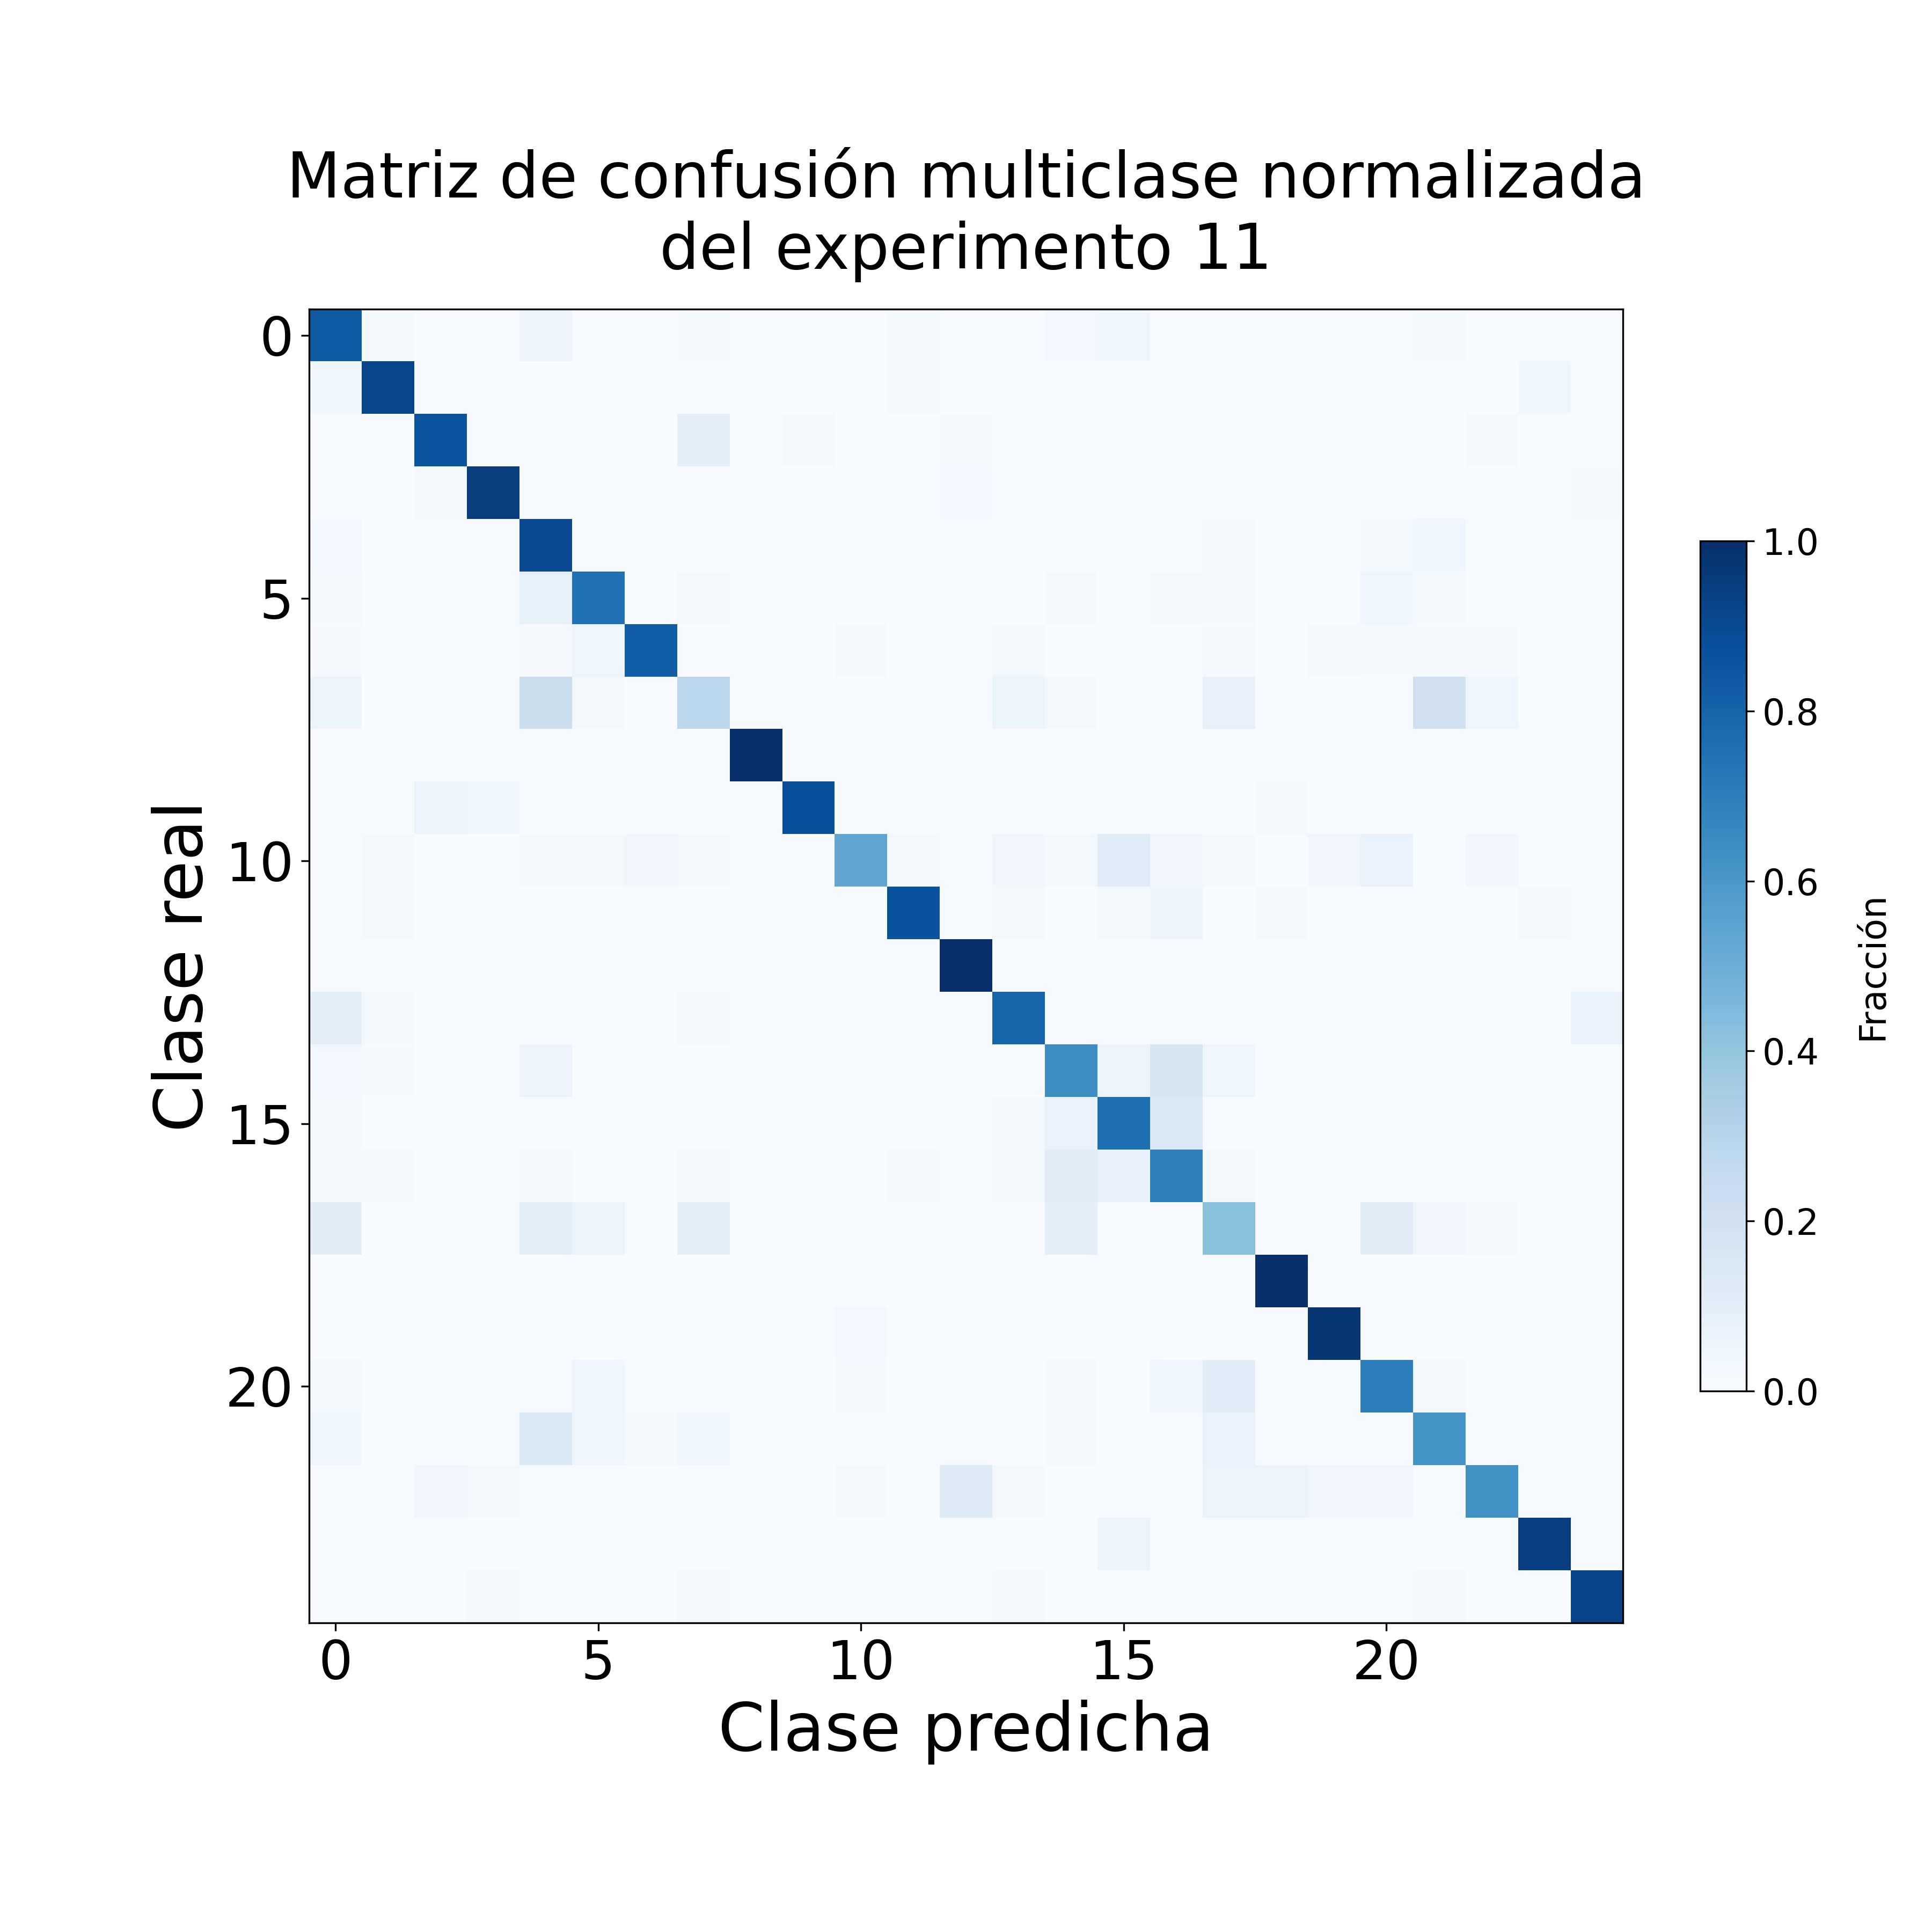
\includegraphics[width=\textwidth]{figures/Experiments_logs/confusion_matrix_05-07-0857.png}
        \caption{}
        \label{fig:confusion_matrix_05-07-0857}
    \end{subfigure}
    \hfill
    \begin{subfigure}{0.45\textwidth}
        \centering
        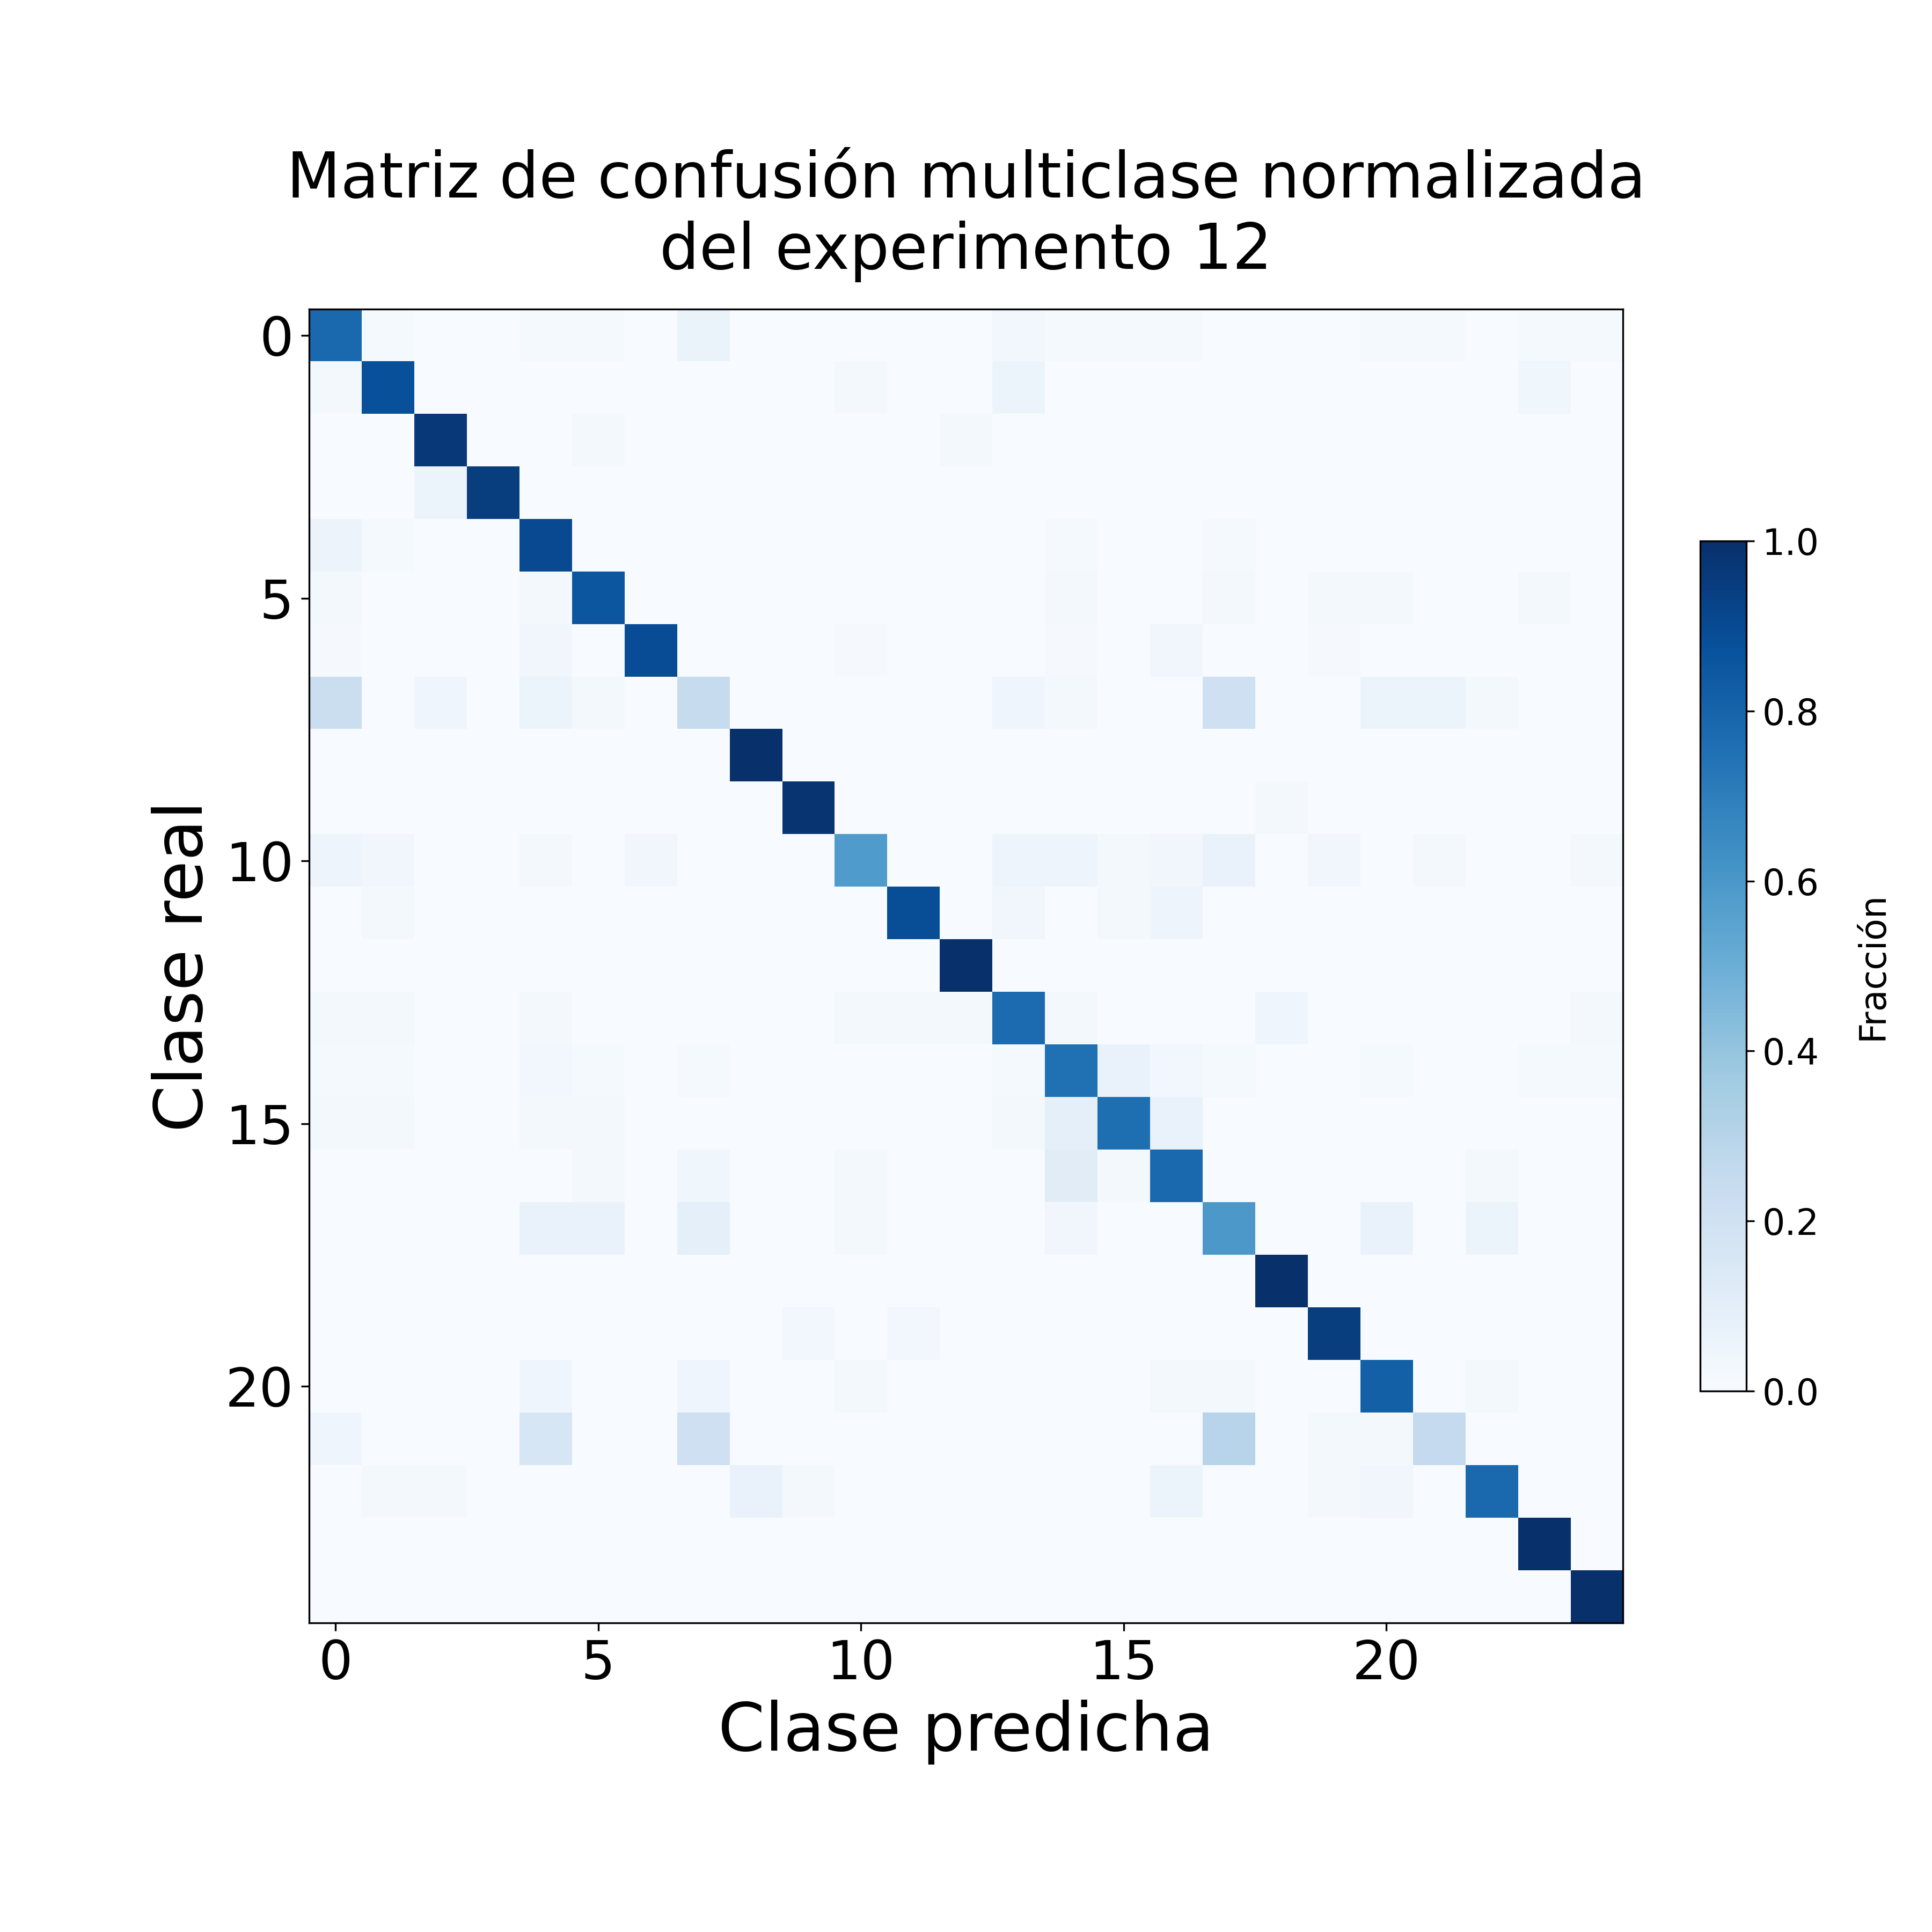
\includegraphics[width=\textwidth]{figures/Experiments_logs/confusion_matrix_05-07-1304.png}
        \caption{}
        \label{fig:confusion_matrix_05-07-1304}
    \end{subfigure}

    \vspace{0.08cm}

    \begin{subfigure}{0.45\textwidth}
        \centering
        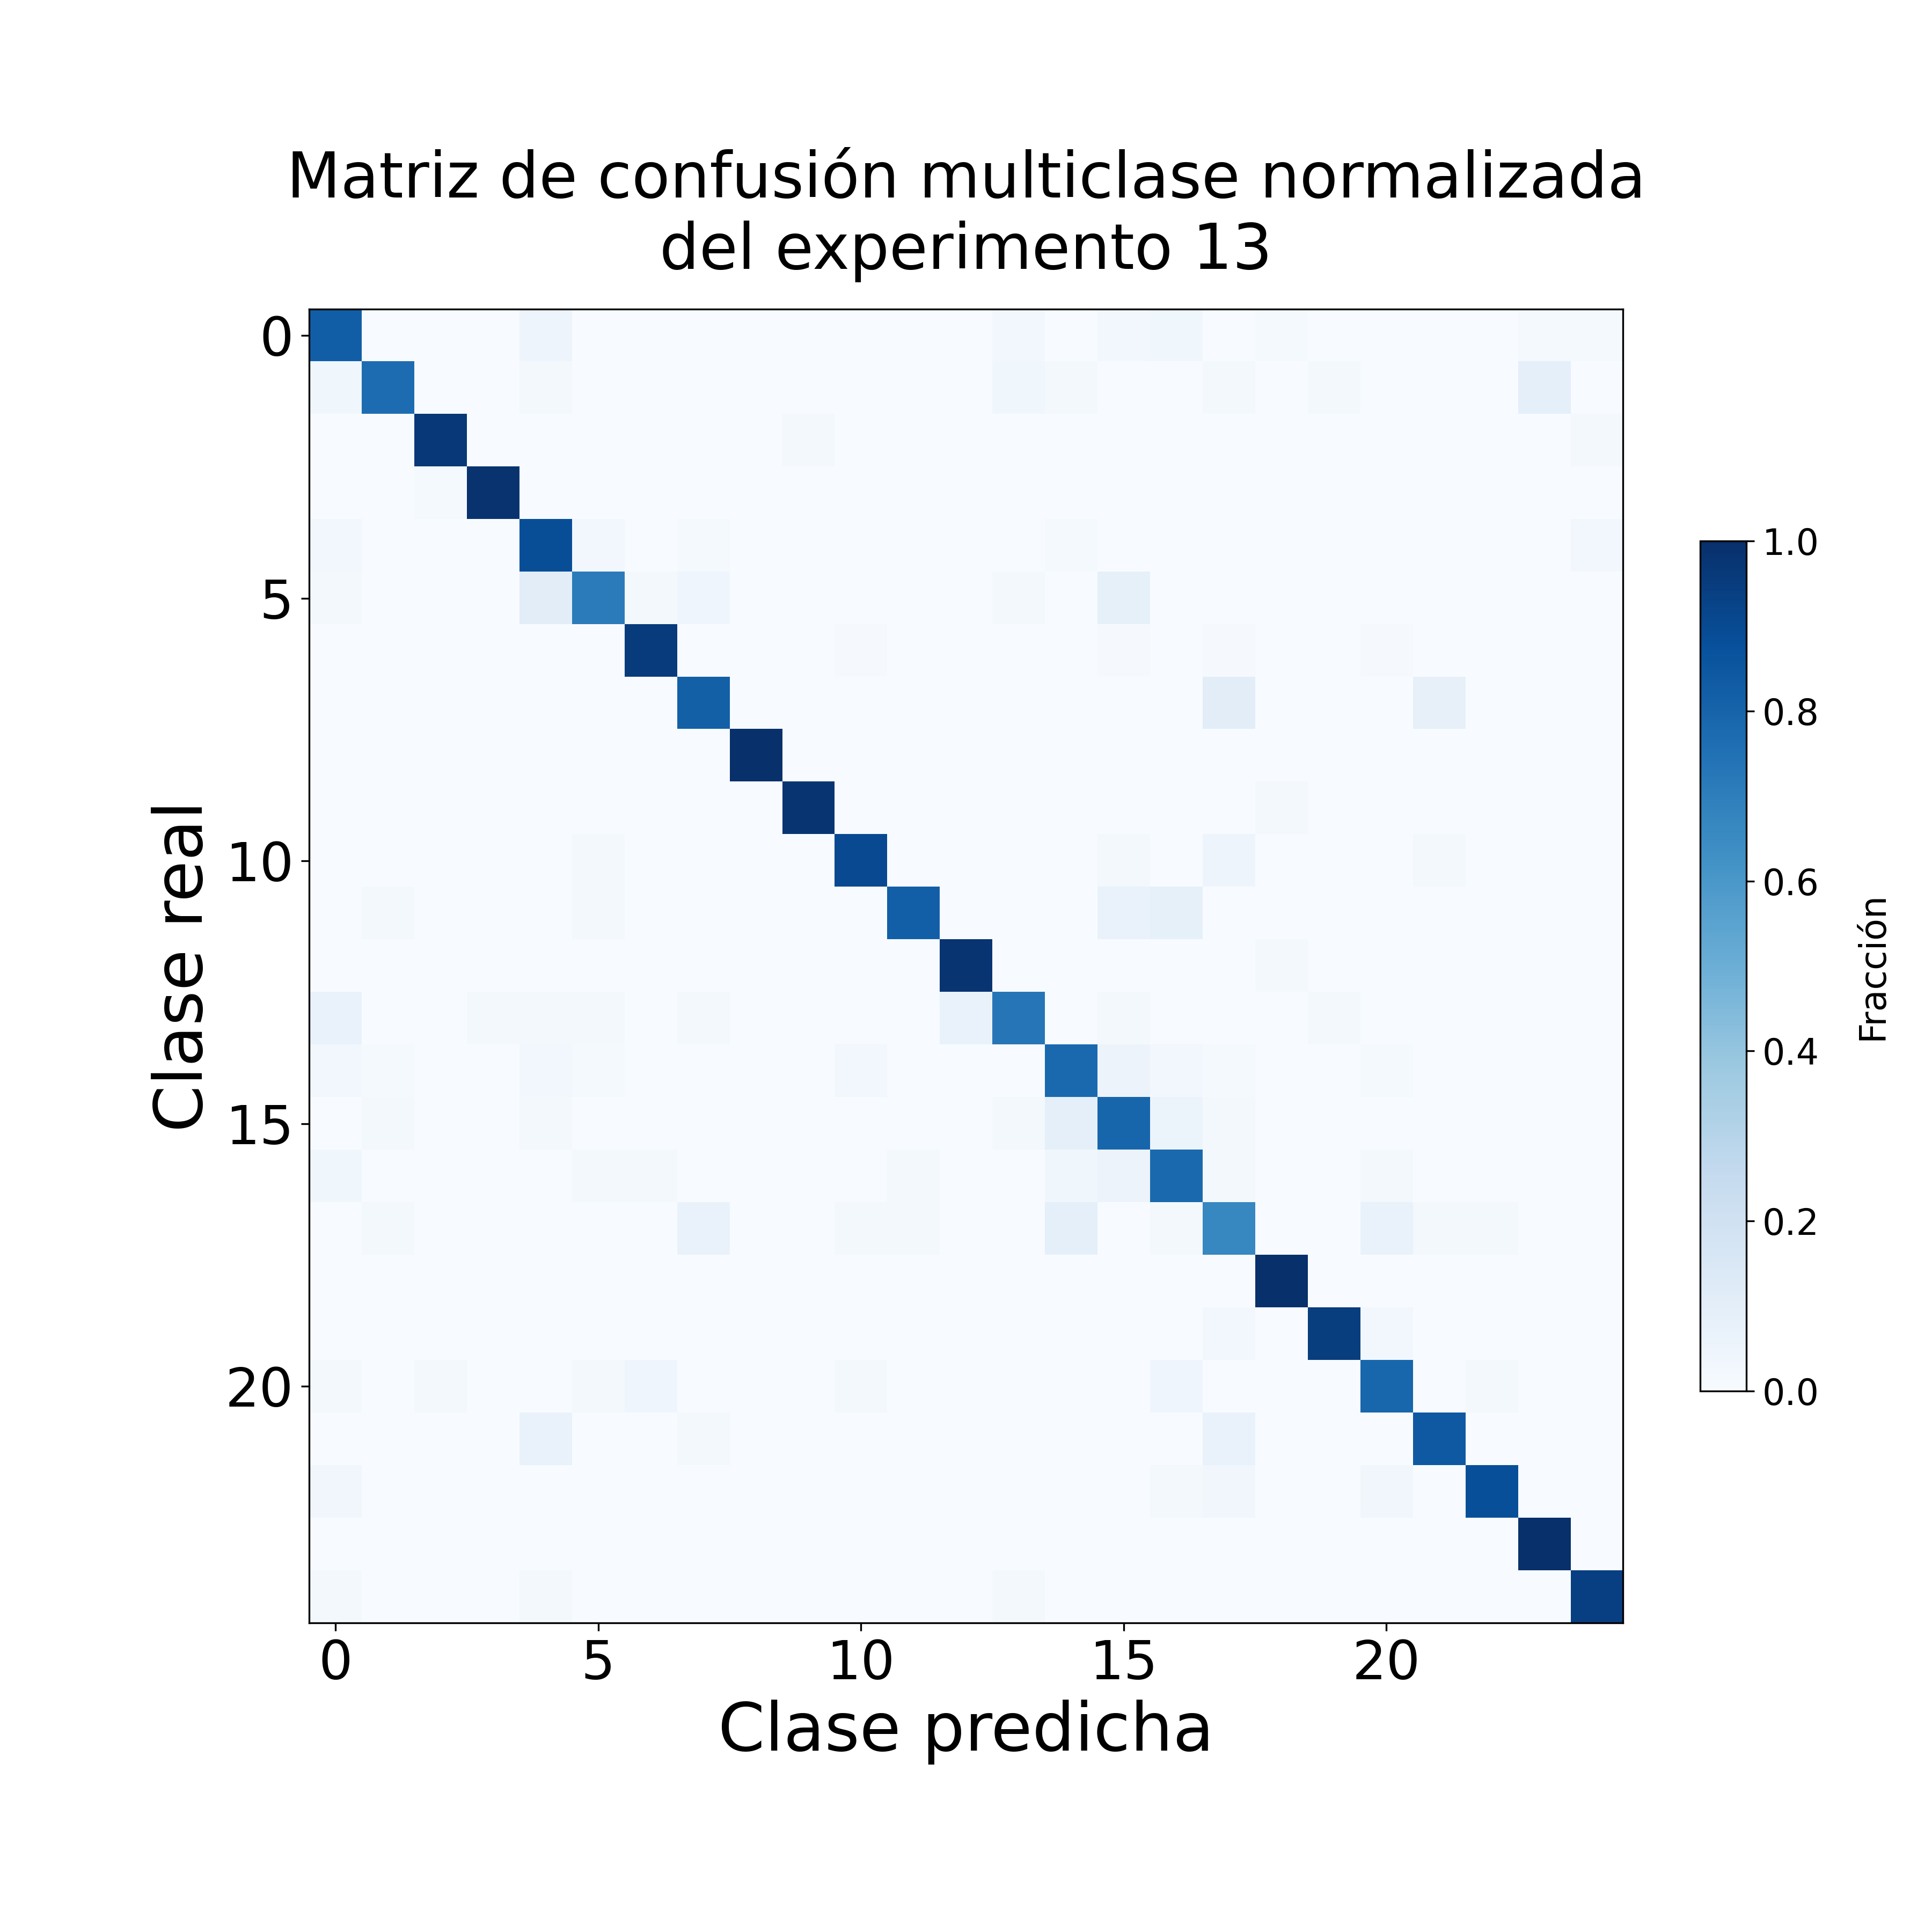
\includegraphics[width=\textwidth]{figures/Experiments_logs/confusion_matrix_05-08-1400.png}
        \caption{}
        \label{fig:confusion_matrix_05-08-1400}
    \end{subfigure}
    \hfill
    \begin{subfigure}{0.45\textwidth}
        \centering
        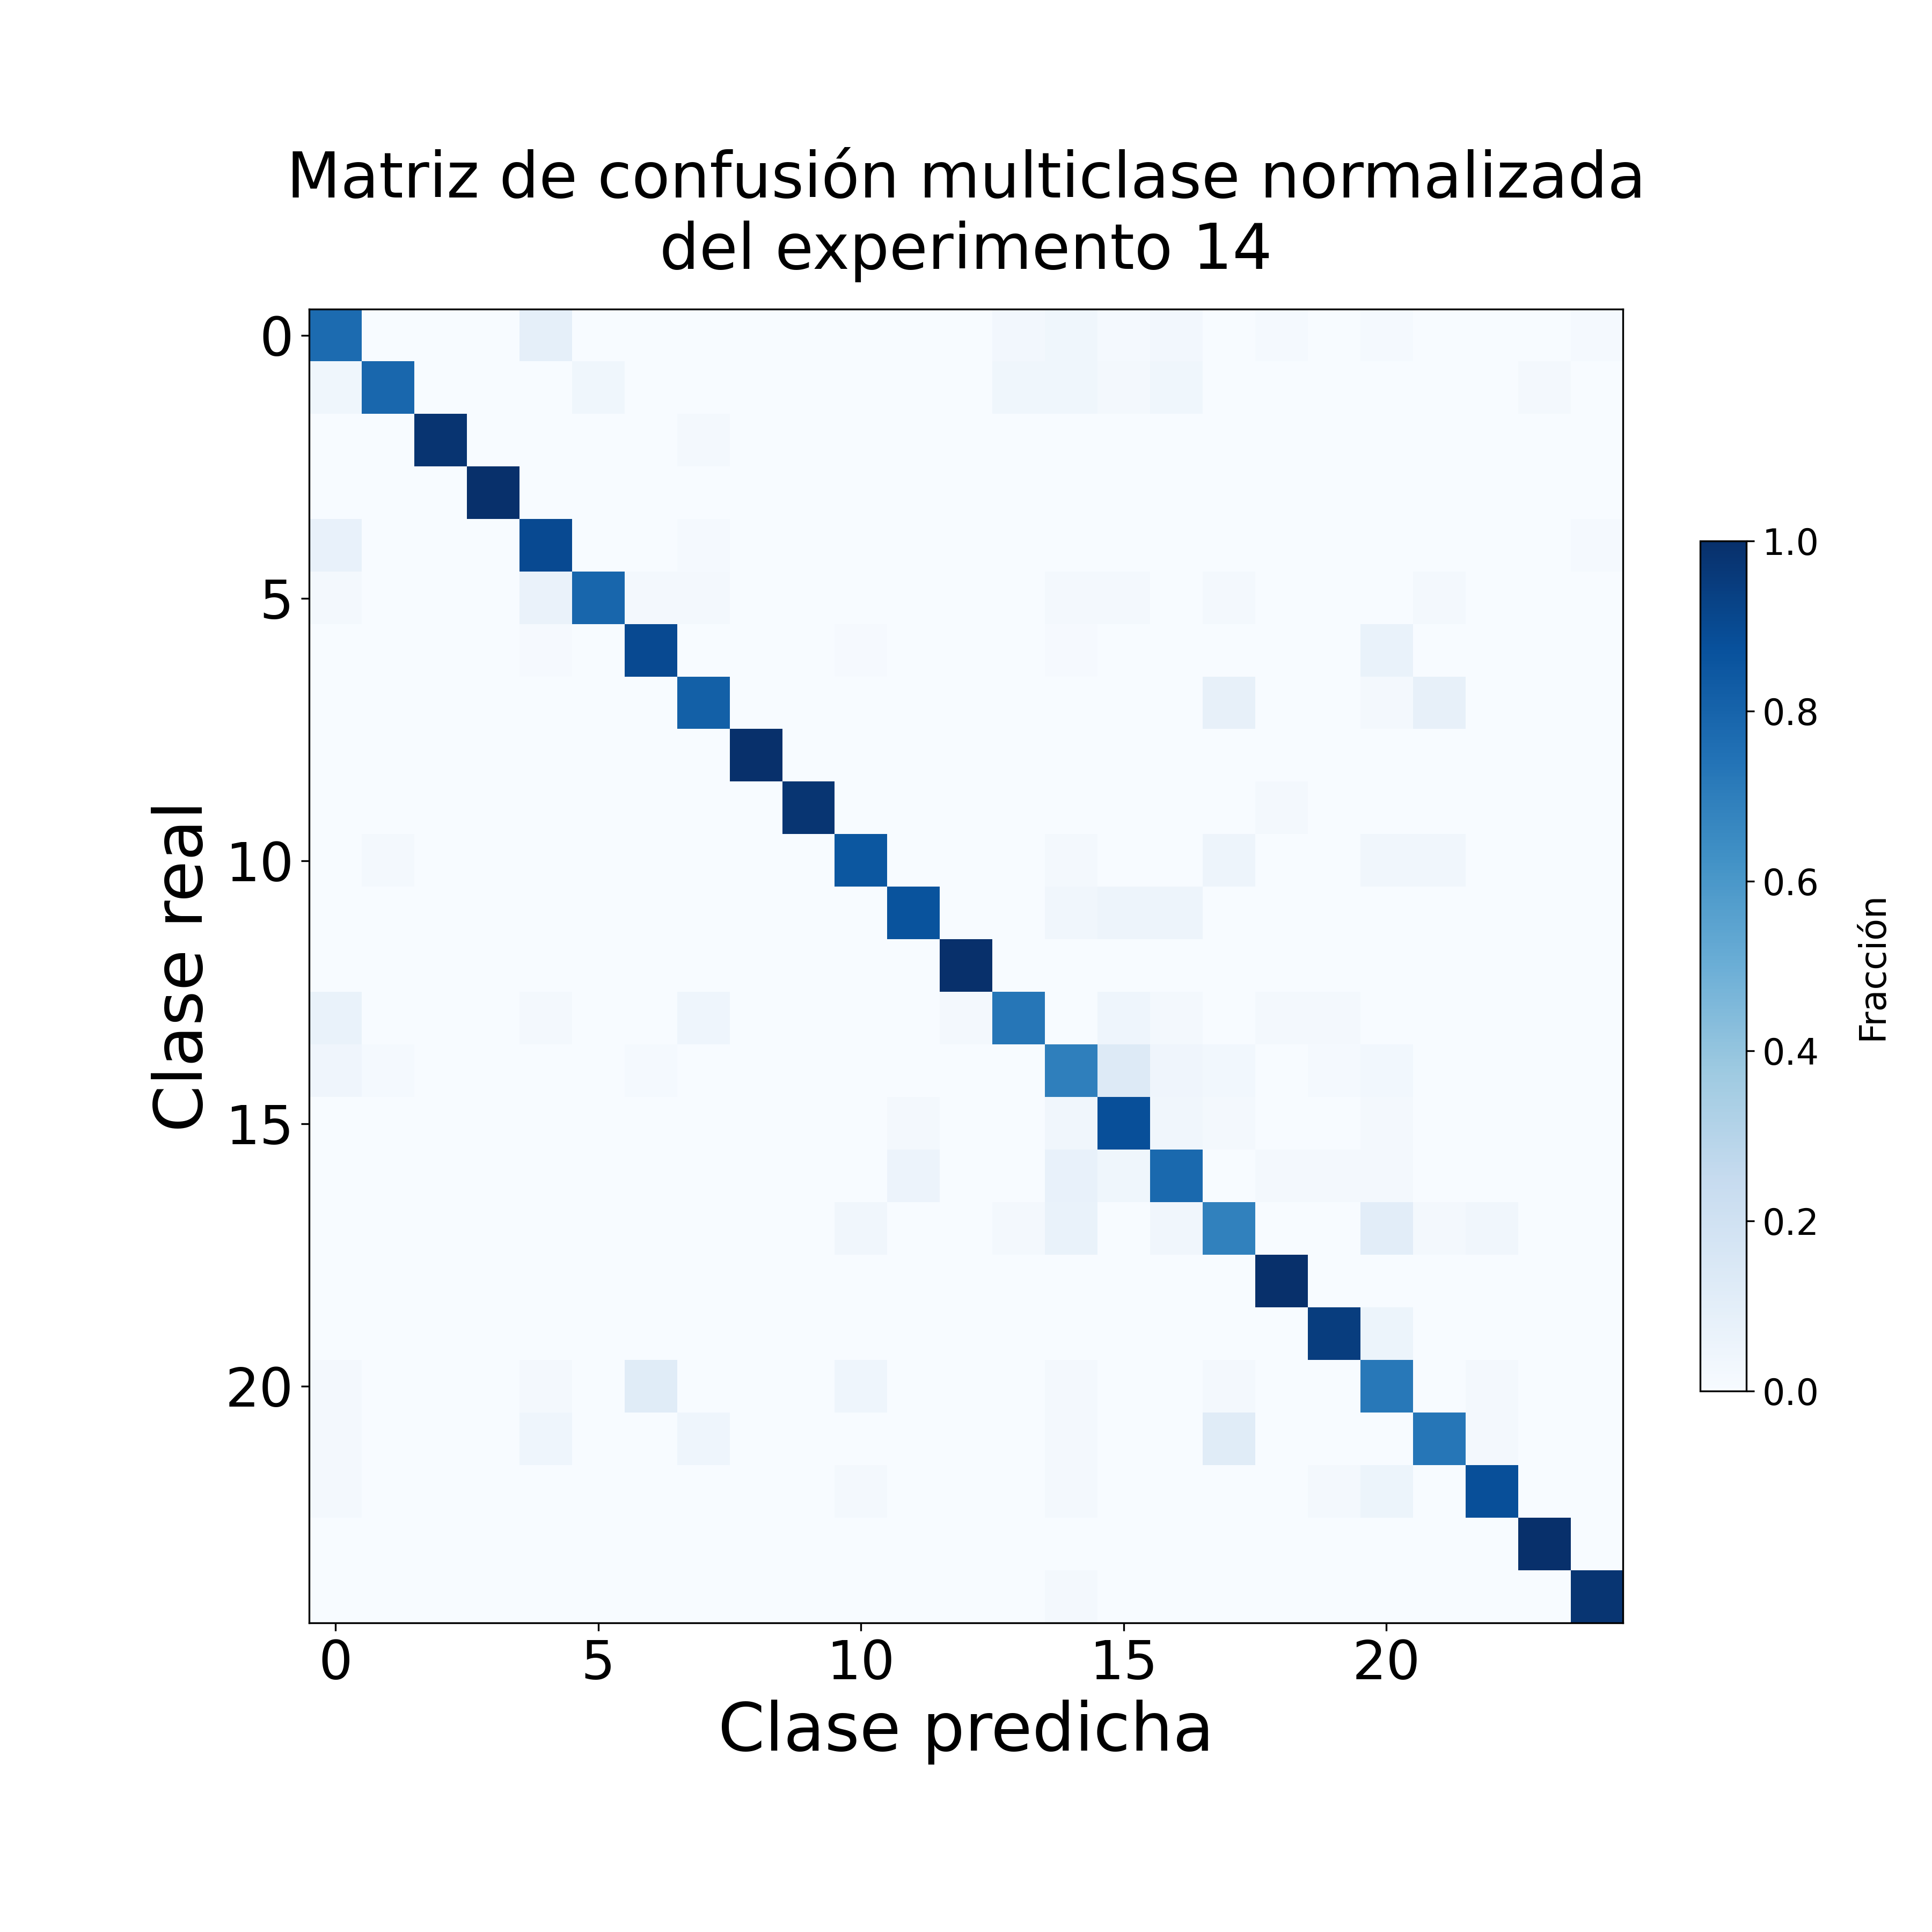
\includegraphics[width=\textwidth]{figures/Experiments_logs/confusion_matrix_05-11-0958.png}
        \caption{}
        \label{fig:confusion_matrix_05-11-0958}
    \end{subfigure}

     \vspace{0.08cm}

    \begin{subfigure}{0.45\textwidth}
        \centering
        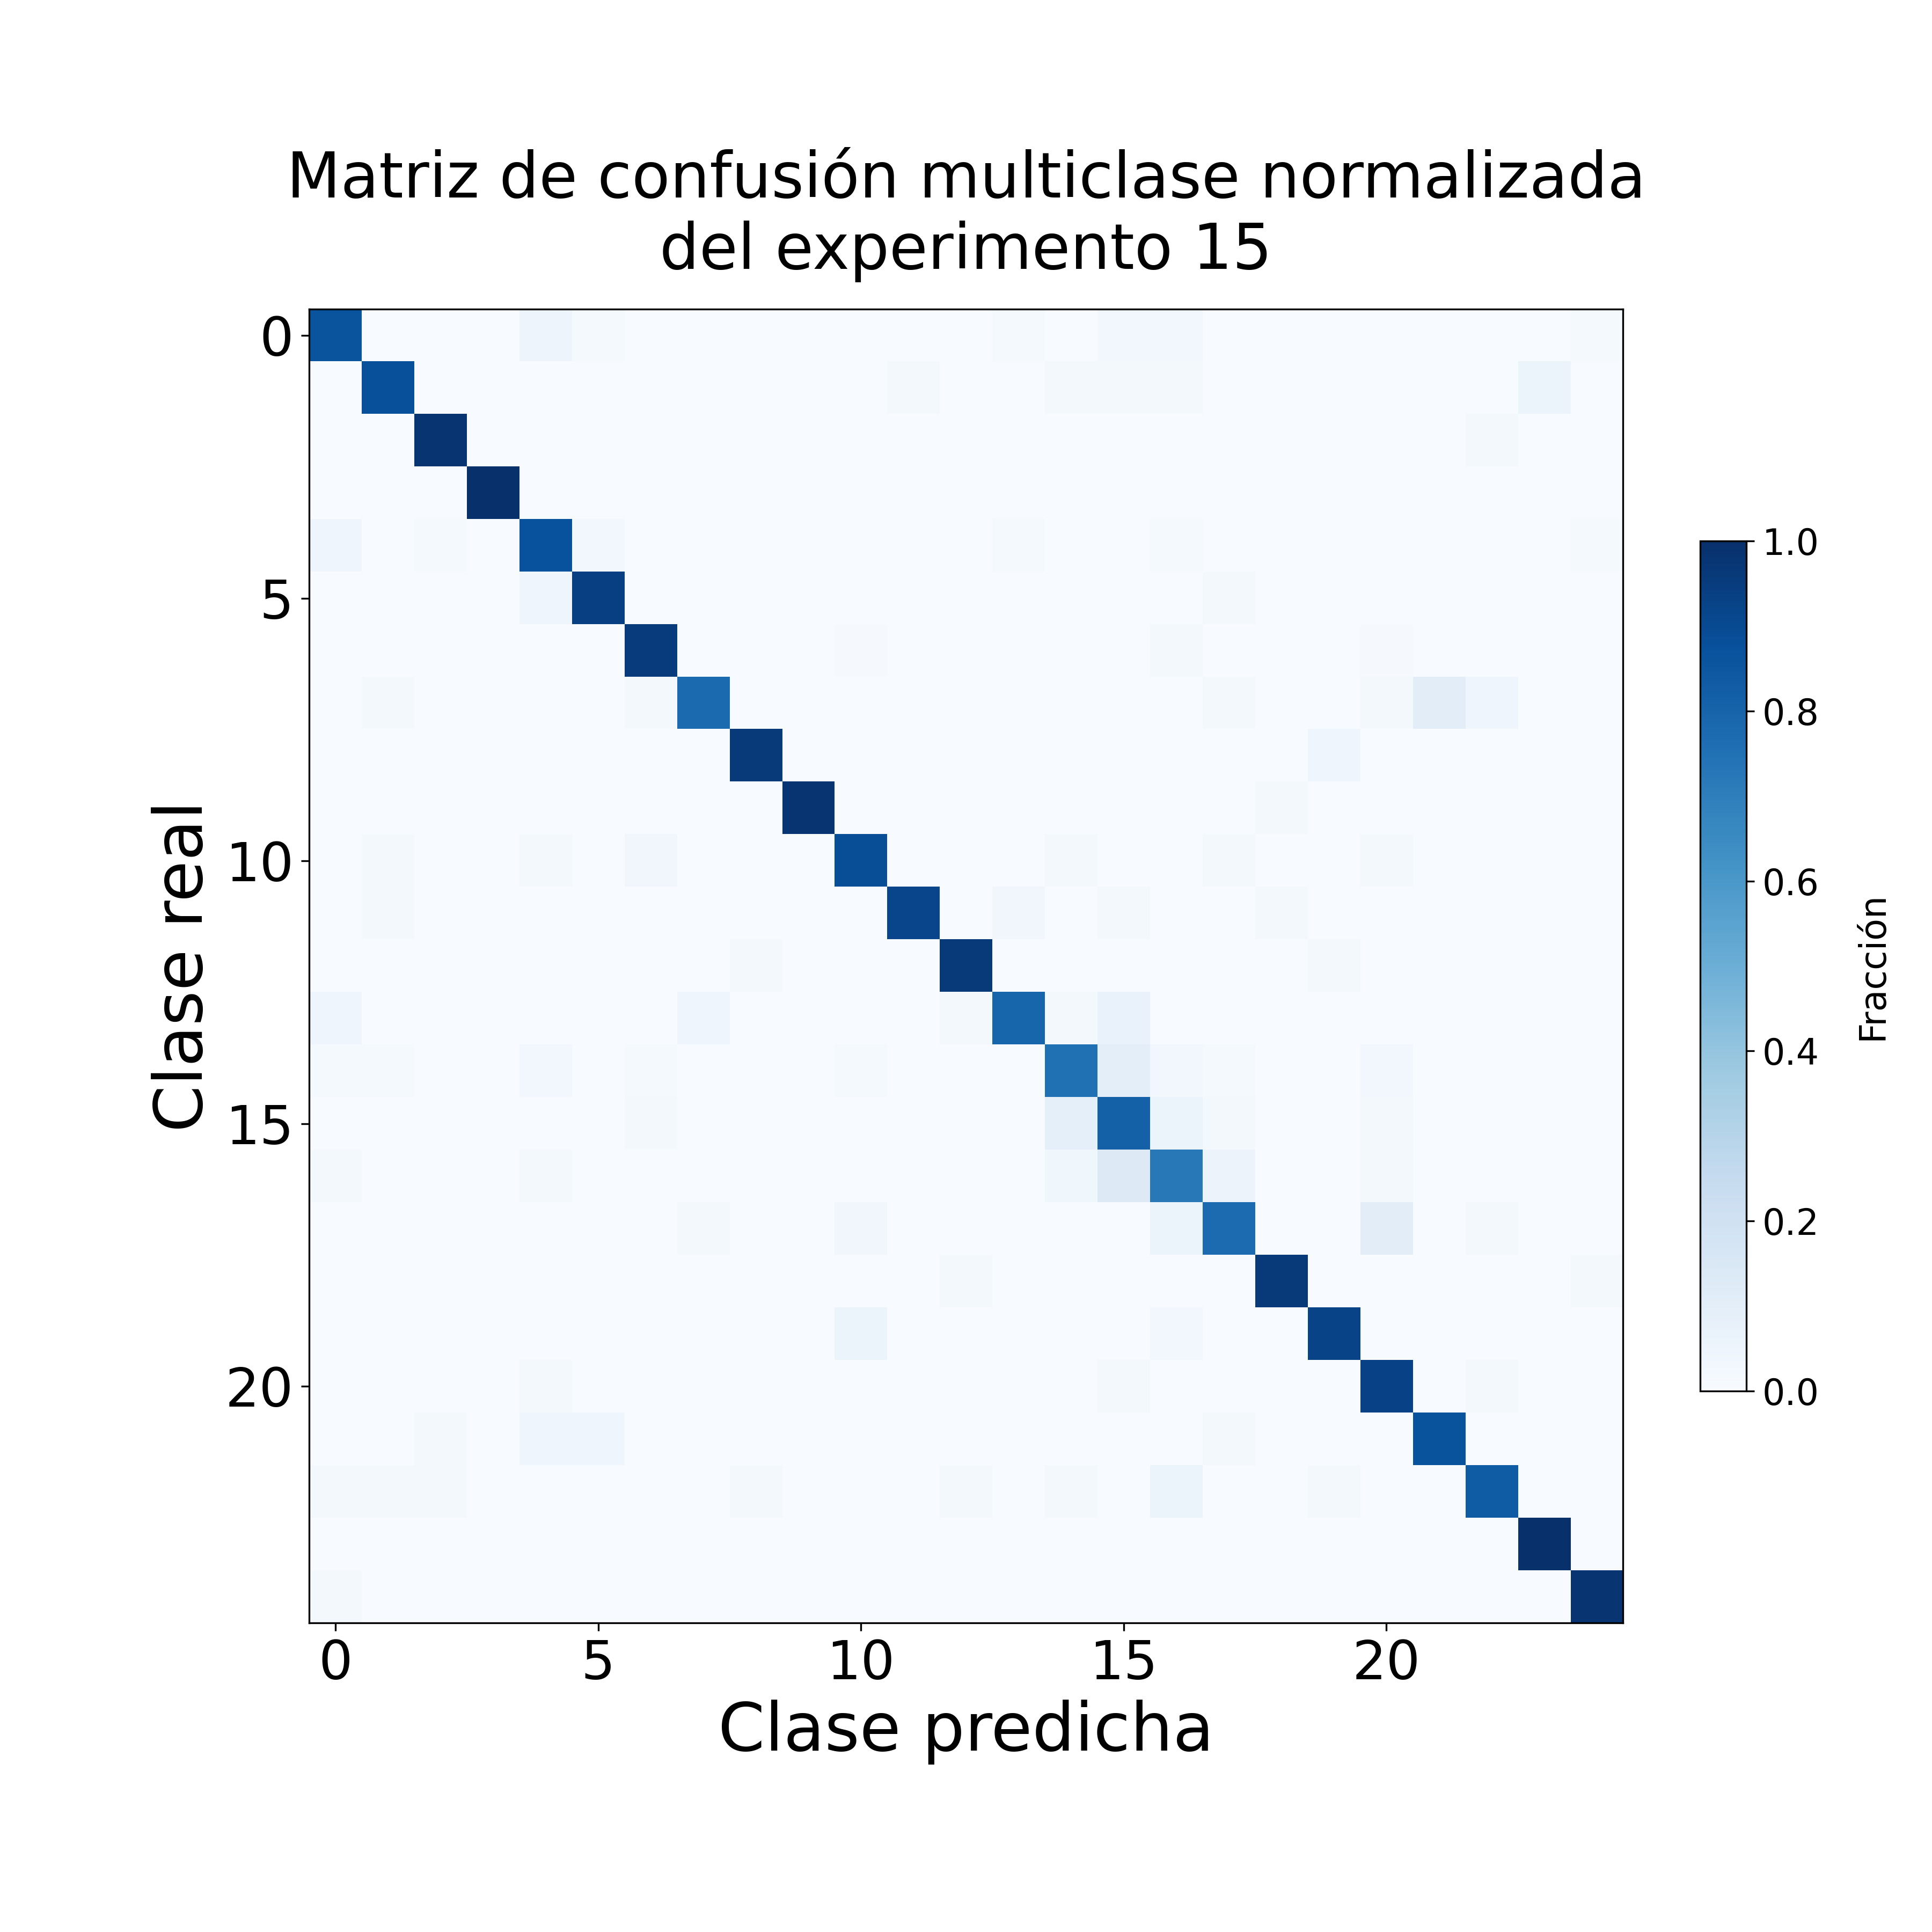
\includegraphics[width=\textwidth]{figures/Experiments_logs/confusion_matrix_05-11-1101.png}
        \caption{}
        \label{fig:confusion_matrix_05-11-1101}
    \end{subfigure}
    
    \caption{Matrices de confusión de distintos experimentos a los que se le fueron aplicando pequeñas mejoras detalladas en \tabref{tab:ajustes_entrenamiento}. Se puede ver como la diagonal se hace más evidente a medida que se aplican los cambios.}
    \label{fig:confusion_matrix-07-11}
\end{figure}

Las clases difíciles seguían siendo bastante coherentes entre experimentos, objetos alargados o muy parecidos entre sí, como \textit{Measuring Cylinder}, \textit{Volumetric Flask}, \textit{Separating Funnel}, \textit{Test Tube}, \textit{Pipette} y las distintas variantes de \textit{Round Bottom Flask}. Esto era una señal importante, los errores no eran aleatorios, sino que estaban concentrados en formas visualmente parecidas.

\subsection{Hipótesis 4}

La cuarta hipótesis fue que el modelo no necesitaba solo más capacidad, sino ver variaciones suaves de esos objetos durante el entrenamiento. Si el modelo confundía clases parecidas por pequeñas diferencias de forma, orientación o visibilidad, entonces una \textit{data augmentation} más adecuada podía ayudar a aprender representaciones más robustas.

Por eso se introdujo una opción de aumento \texttt{light}, con rotaciones pequeñas y borrado aleatorio bajo. No se buscaba deformar agresivamente los objetos, porque en este dataset la geometría importa mucho. La idea era justamente la contraria, simular variaciones más ligeras sin destruir la clase.

\section{Salto con data augmentation light}

El cambio más importante de toda la fase final fue la nueva \textit{data augmentation} suave. Manteniendo la configuración fuerte anterior, se lanzaron cuatro experimentos con seeds distintas:

\begin{table}[H]
\centering
\small
\begin{tabular}{lccccc}
\toprule
\textbf{Experimento} & \textbf{Seed} & \textbf{Mejor acc.} & \textbf{Top-5} & \textbf{Mejor loss} & \textbf{Macro F1} \\
\midrule
\texttt{16} & 55 & 94,54\% & 98,85\% & 0,2684 & 94,64\% \\
\texttt{17} & 42 & 94,19\% & 99,21\% & 0,2503 & 94,26\% \\
\texttt{18} & 69 & 96,05\% & 99,43\% & 0,1997 & 95,94\% \\
\texttt{19} & 111 & 94,26\% & 98,71\% & 0,2634 & 94,28\% \\
\midrule
\textbf{Media} & -- & \textbf{94,76\%} & -- & -- & \textbf{94,78\%} \\
\bottomrule
\end{tabular}
\caption{Resultados con \texttt{augmentation\_name = light}.}
\label{tab:light_augmentation}
\end{table}

\begin{figure}[H]
    \centering

    \begin{subfigure}{0.45\textwidth}
        \centering
        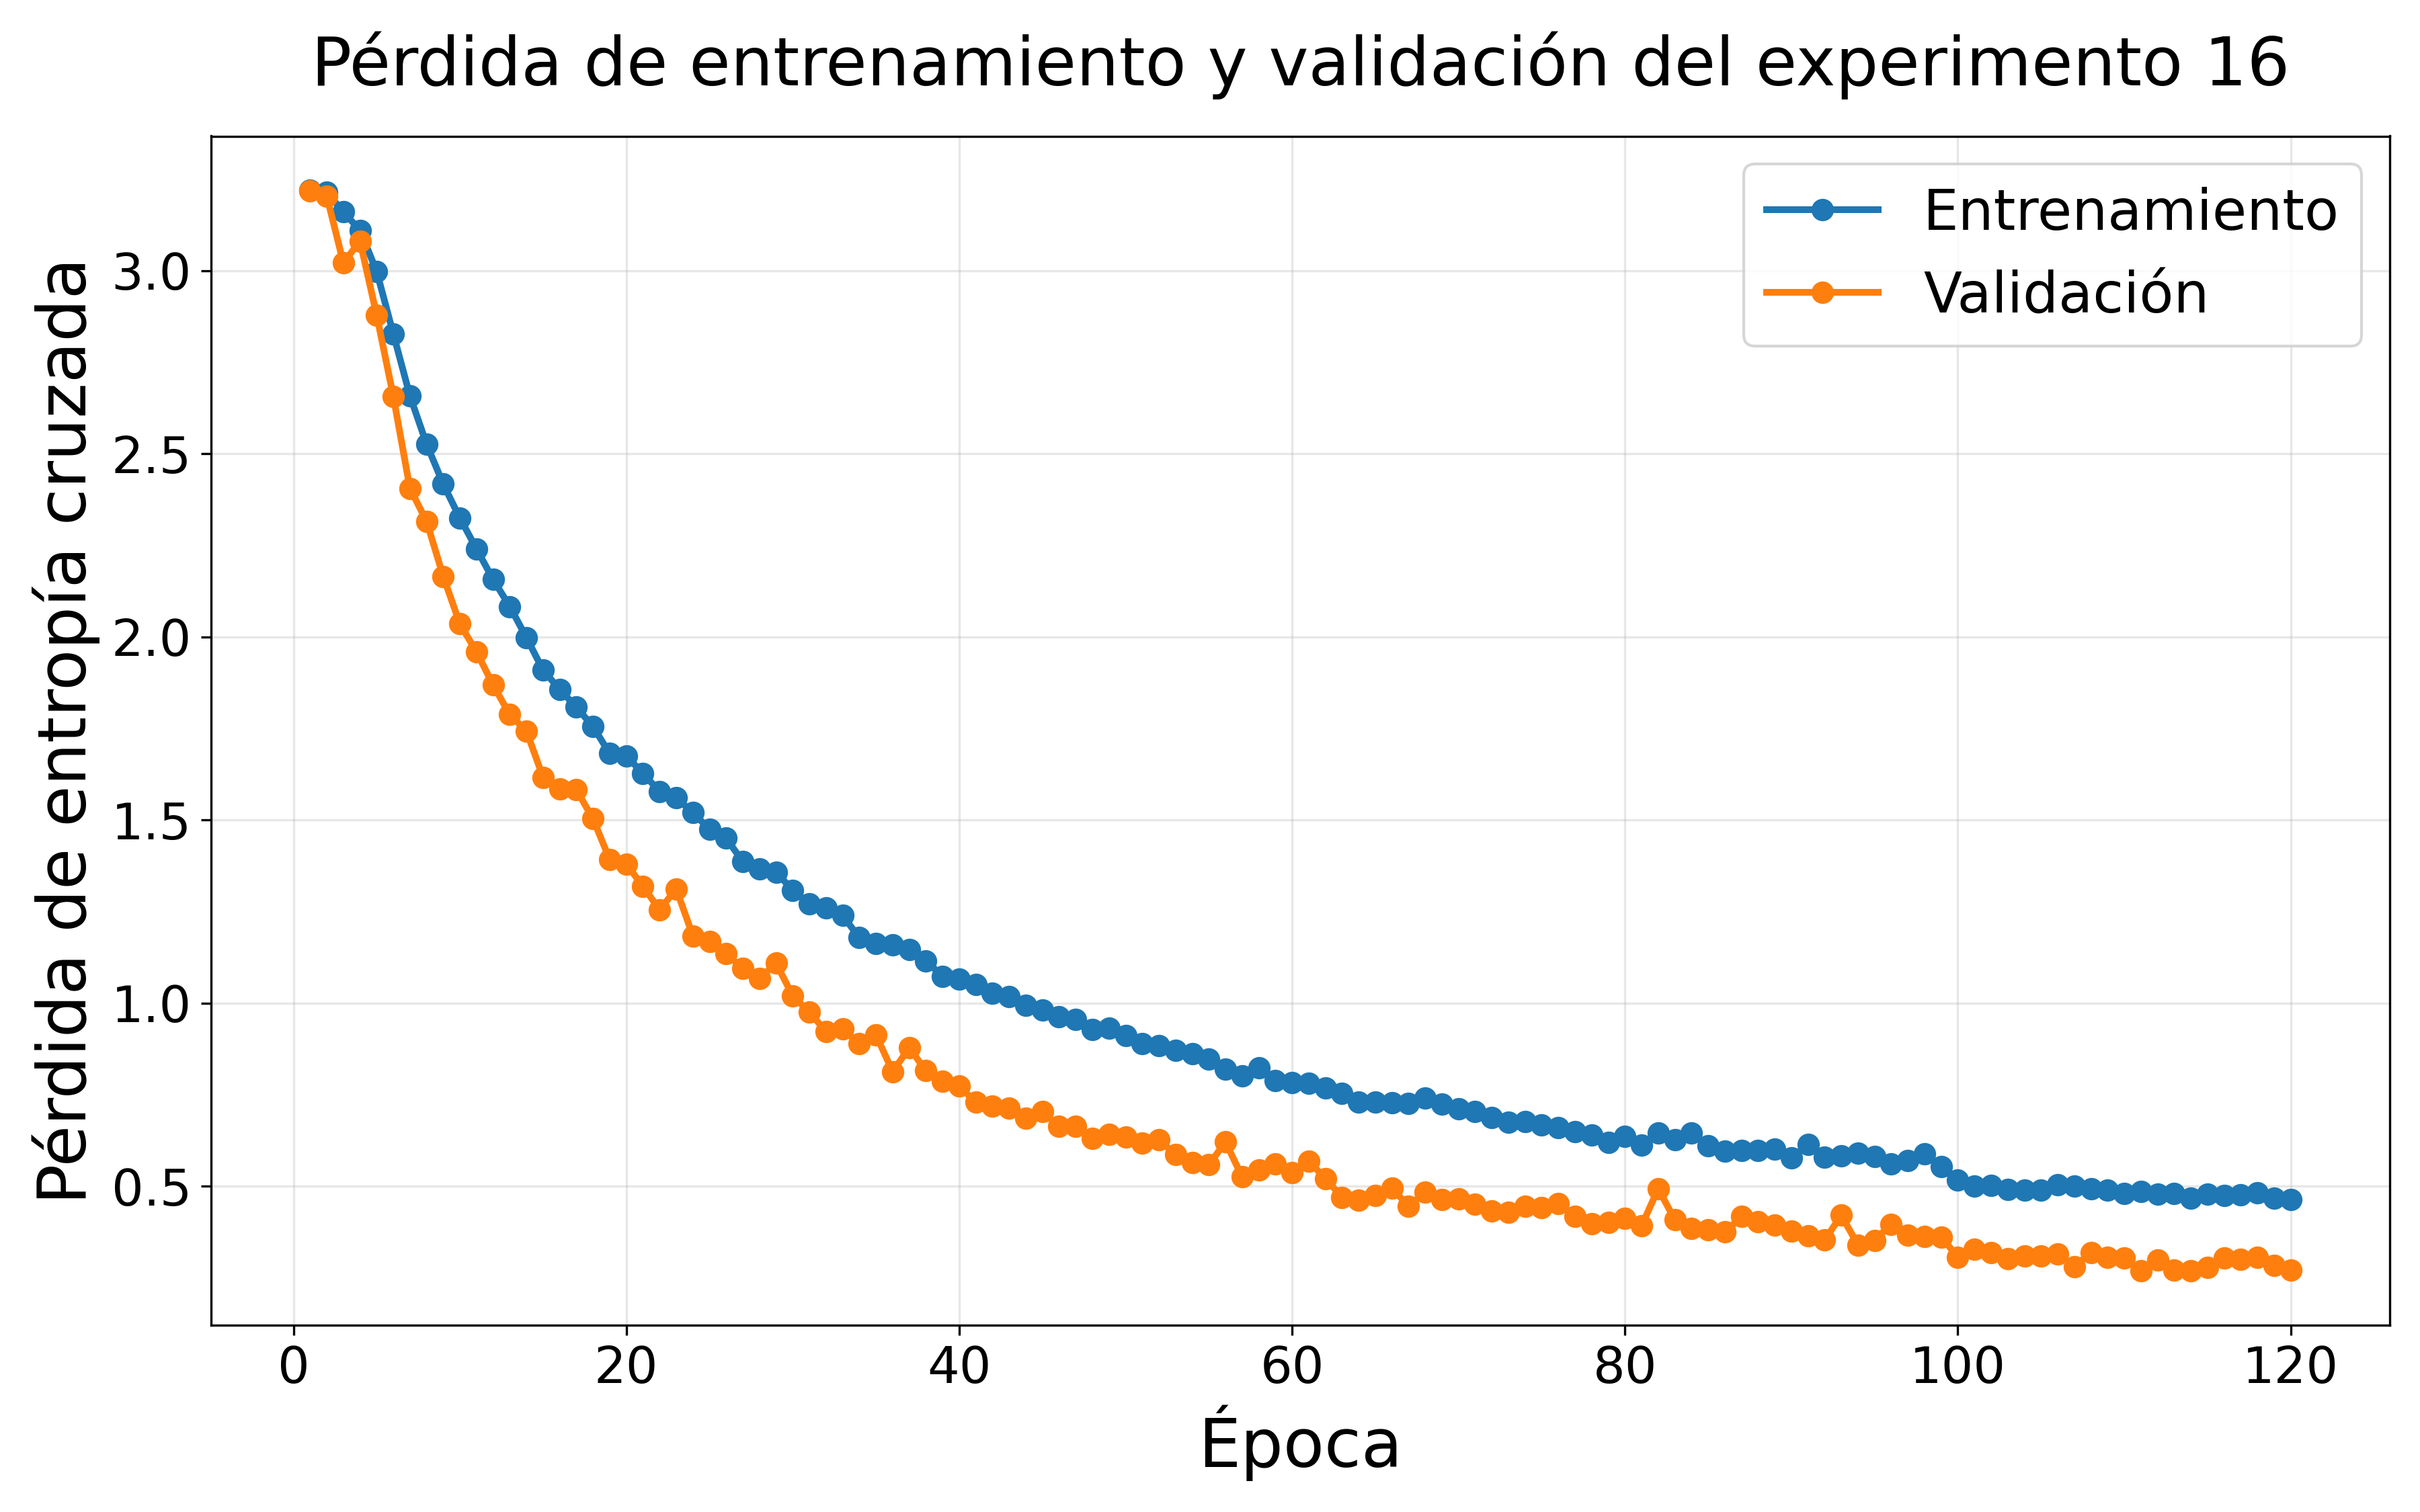
\includegraphics[width=\textwidth]{figures/Experiments_logs/loss_curve_05-14-1025.png}
        \caption{}
        \label{fig:loss_curve_05-14-1025}
    \end{subfigure}
    \hfill
    \begin{subfigure}{0.45\textwidth}
        \centering
        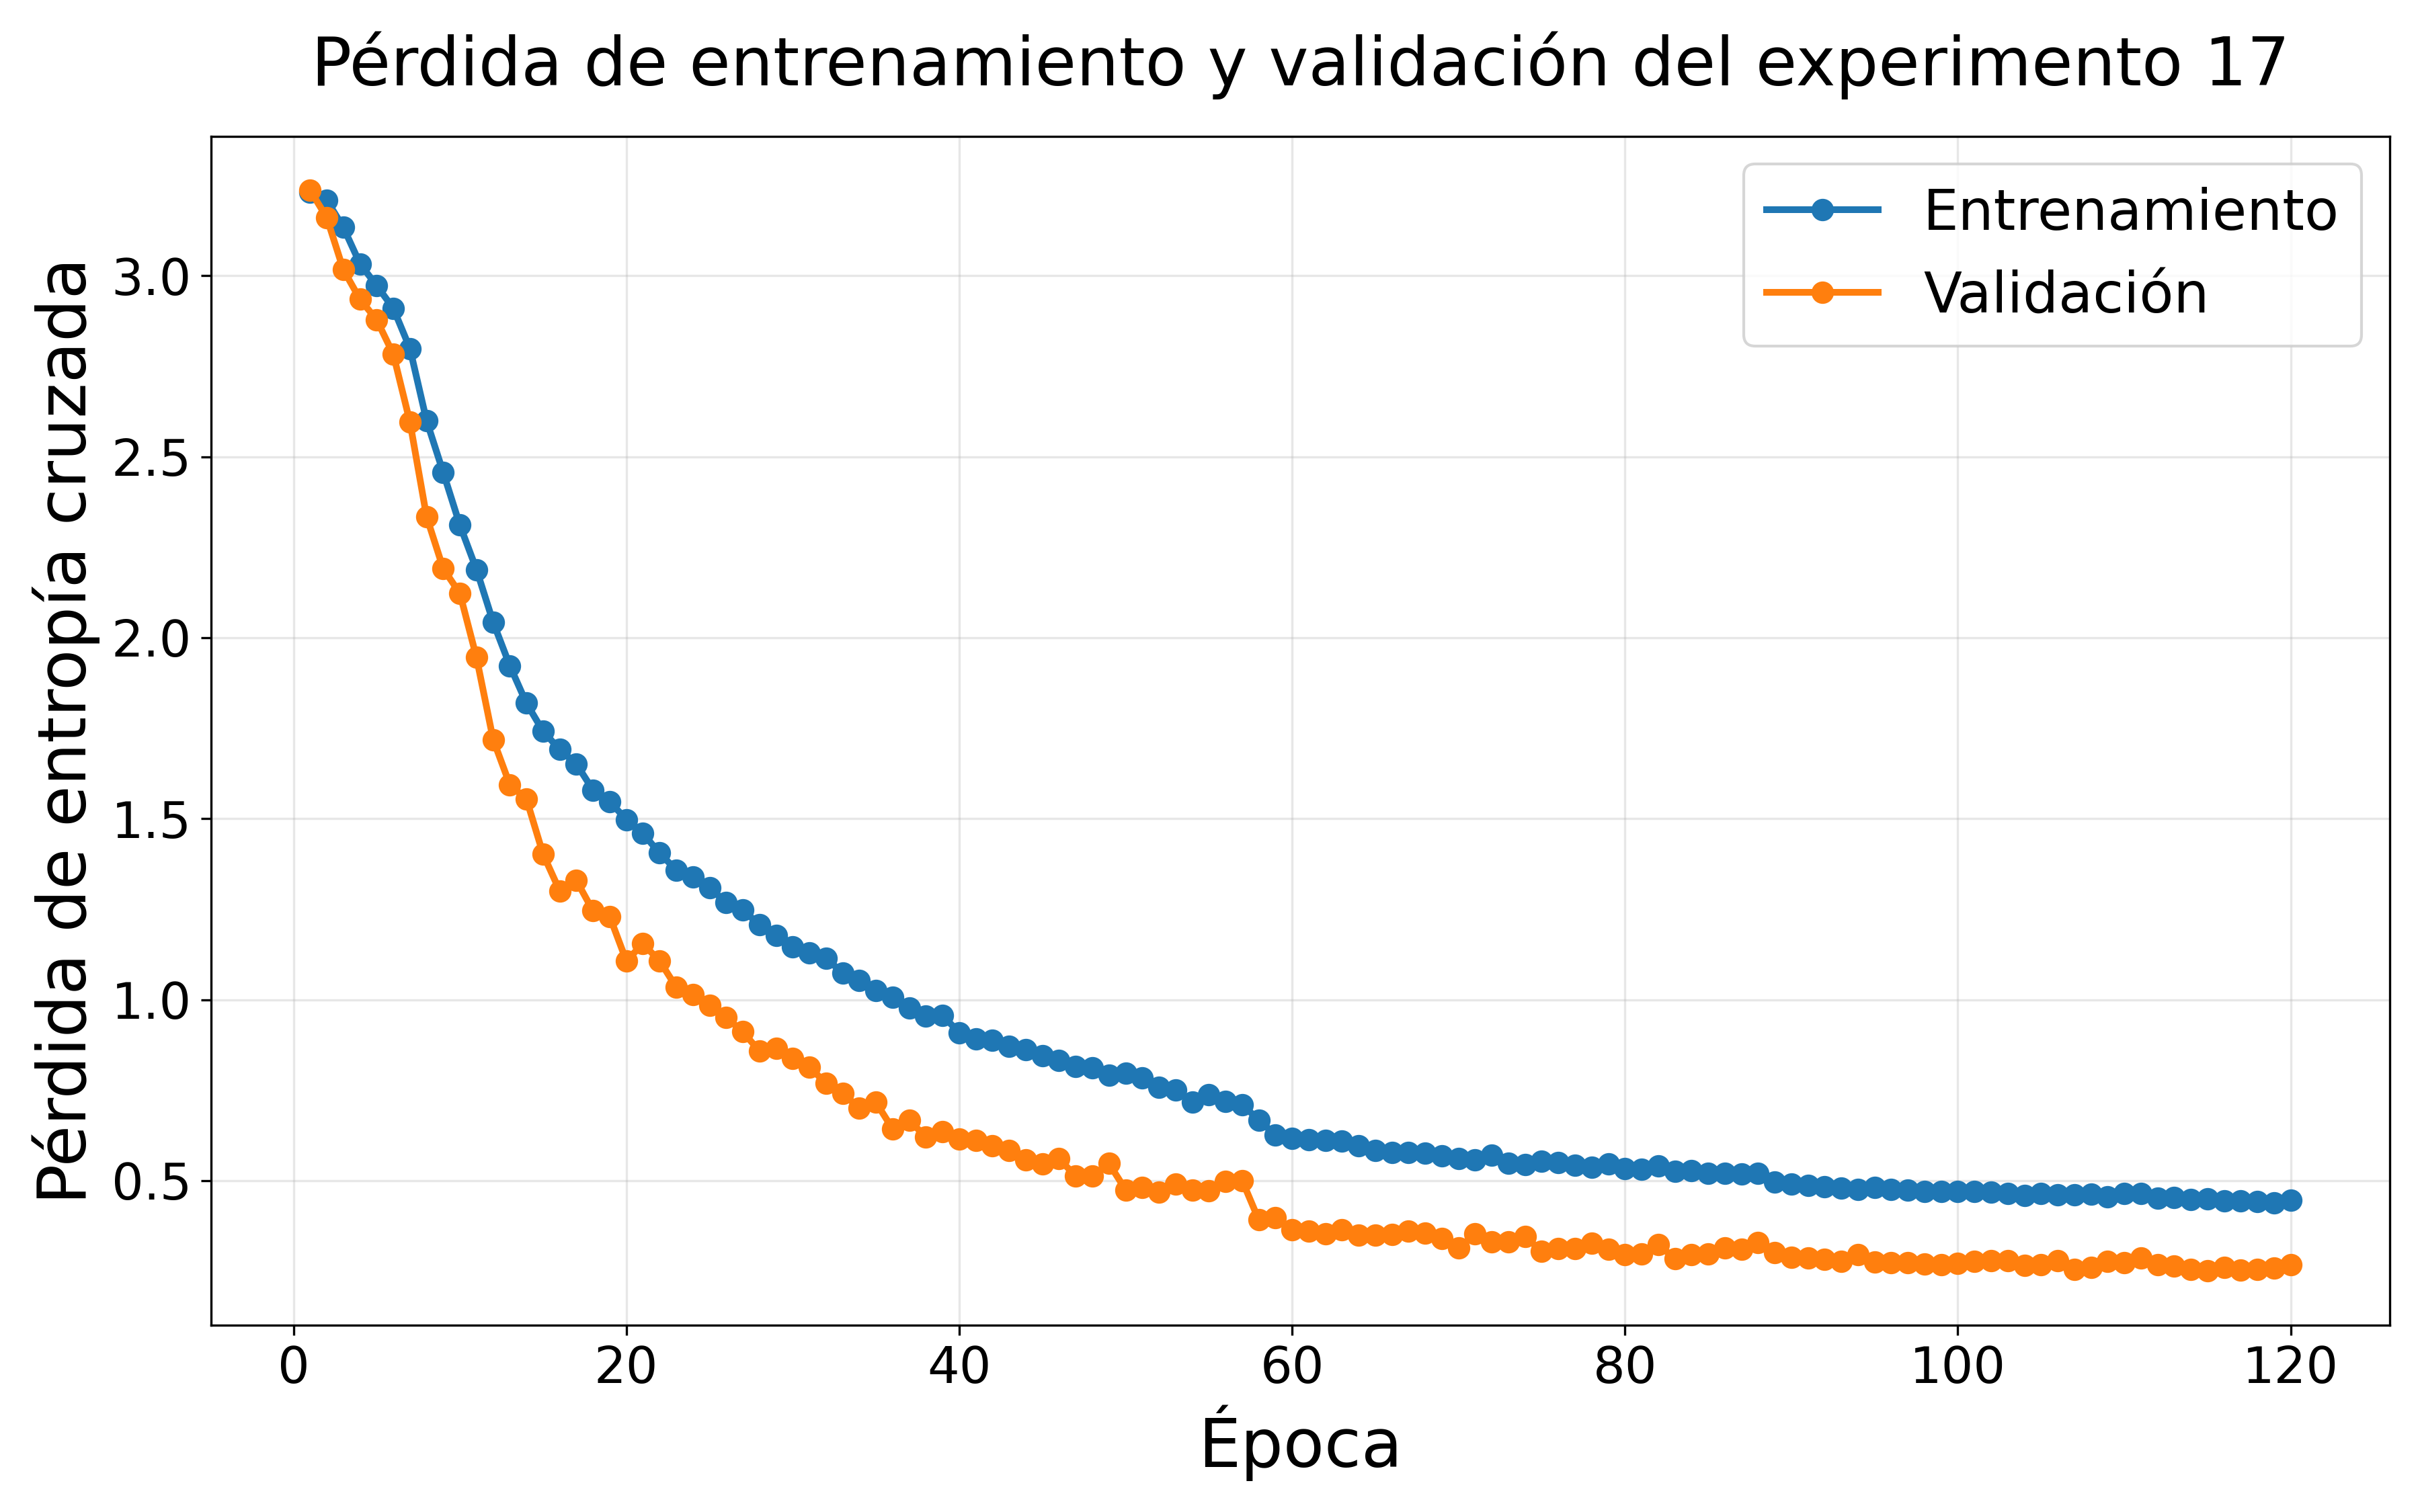
\includegraphics[width=\textwidth]{figures/Experiments_logs/loss_curve_05-14-1026.png}
        \caption{}
        \label{fig:loss_curve_05-14-1026}
    \end{subfigure}

    \vspace{0.4cm}

    \begin{subfigure}{0.45\textwidth}
        \centering
        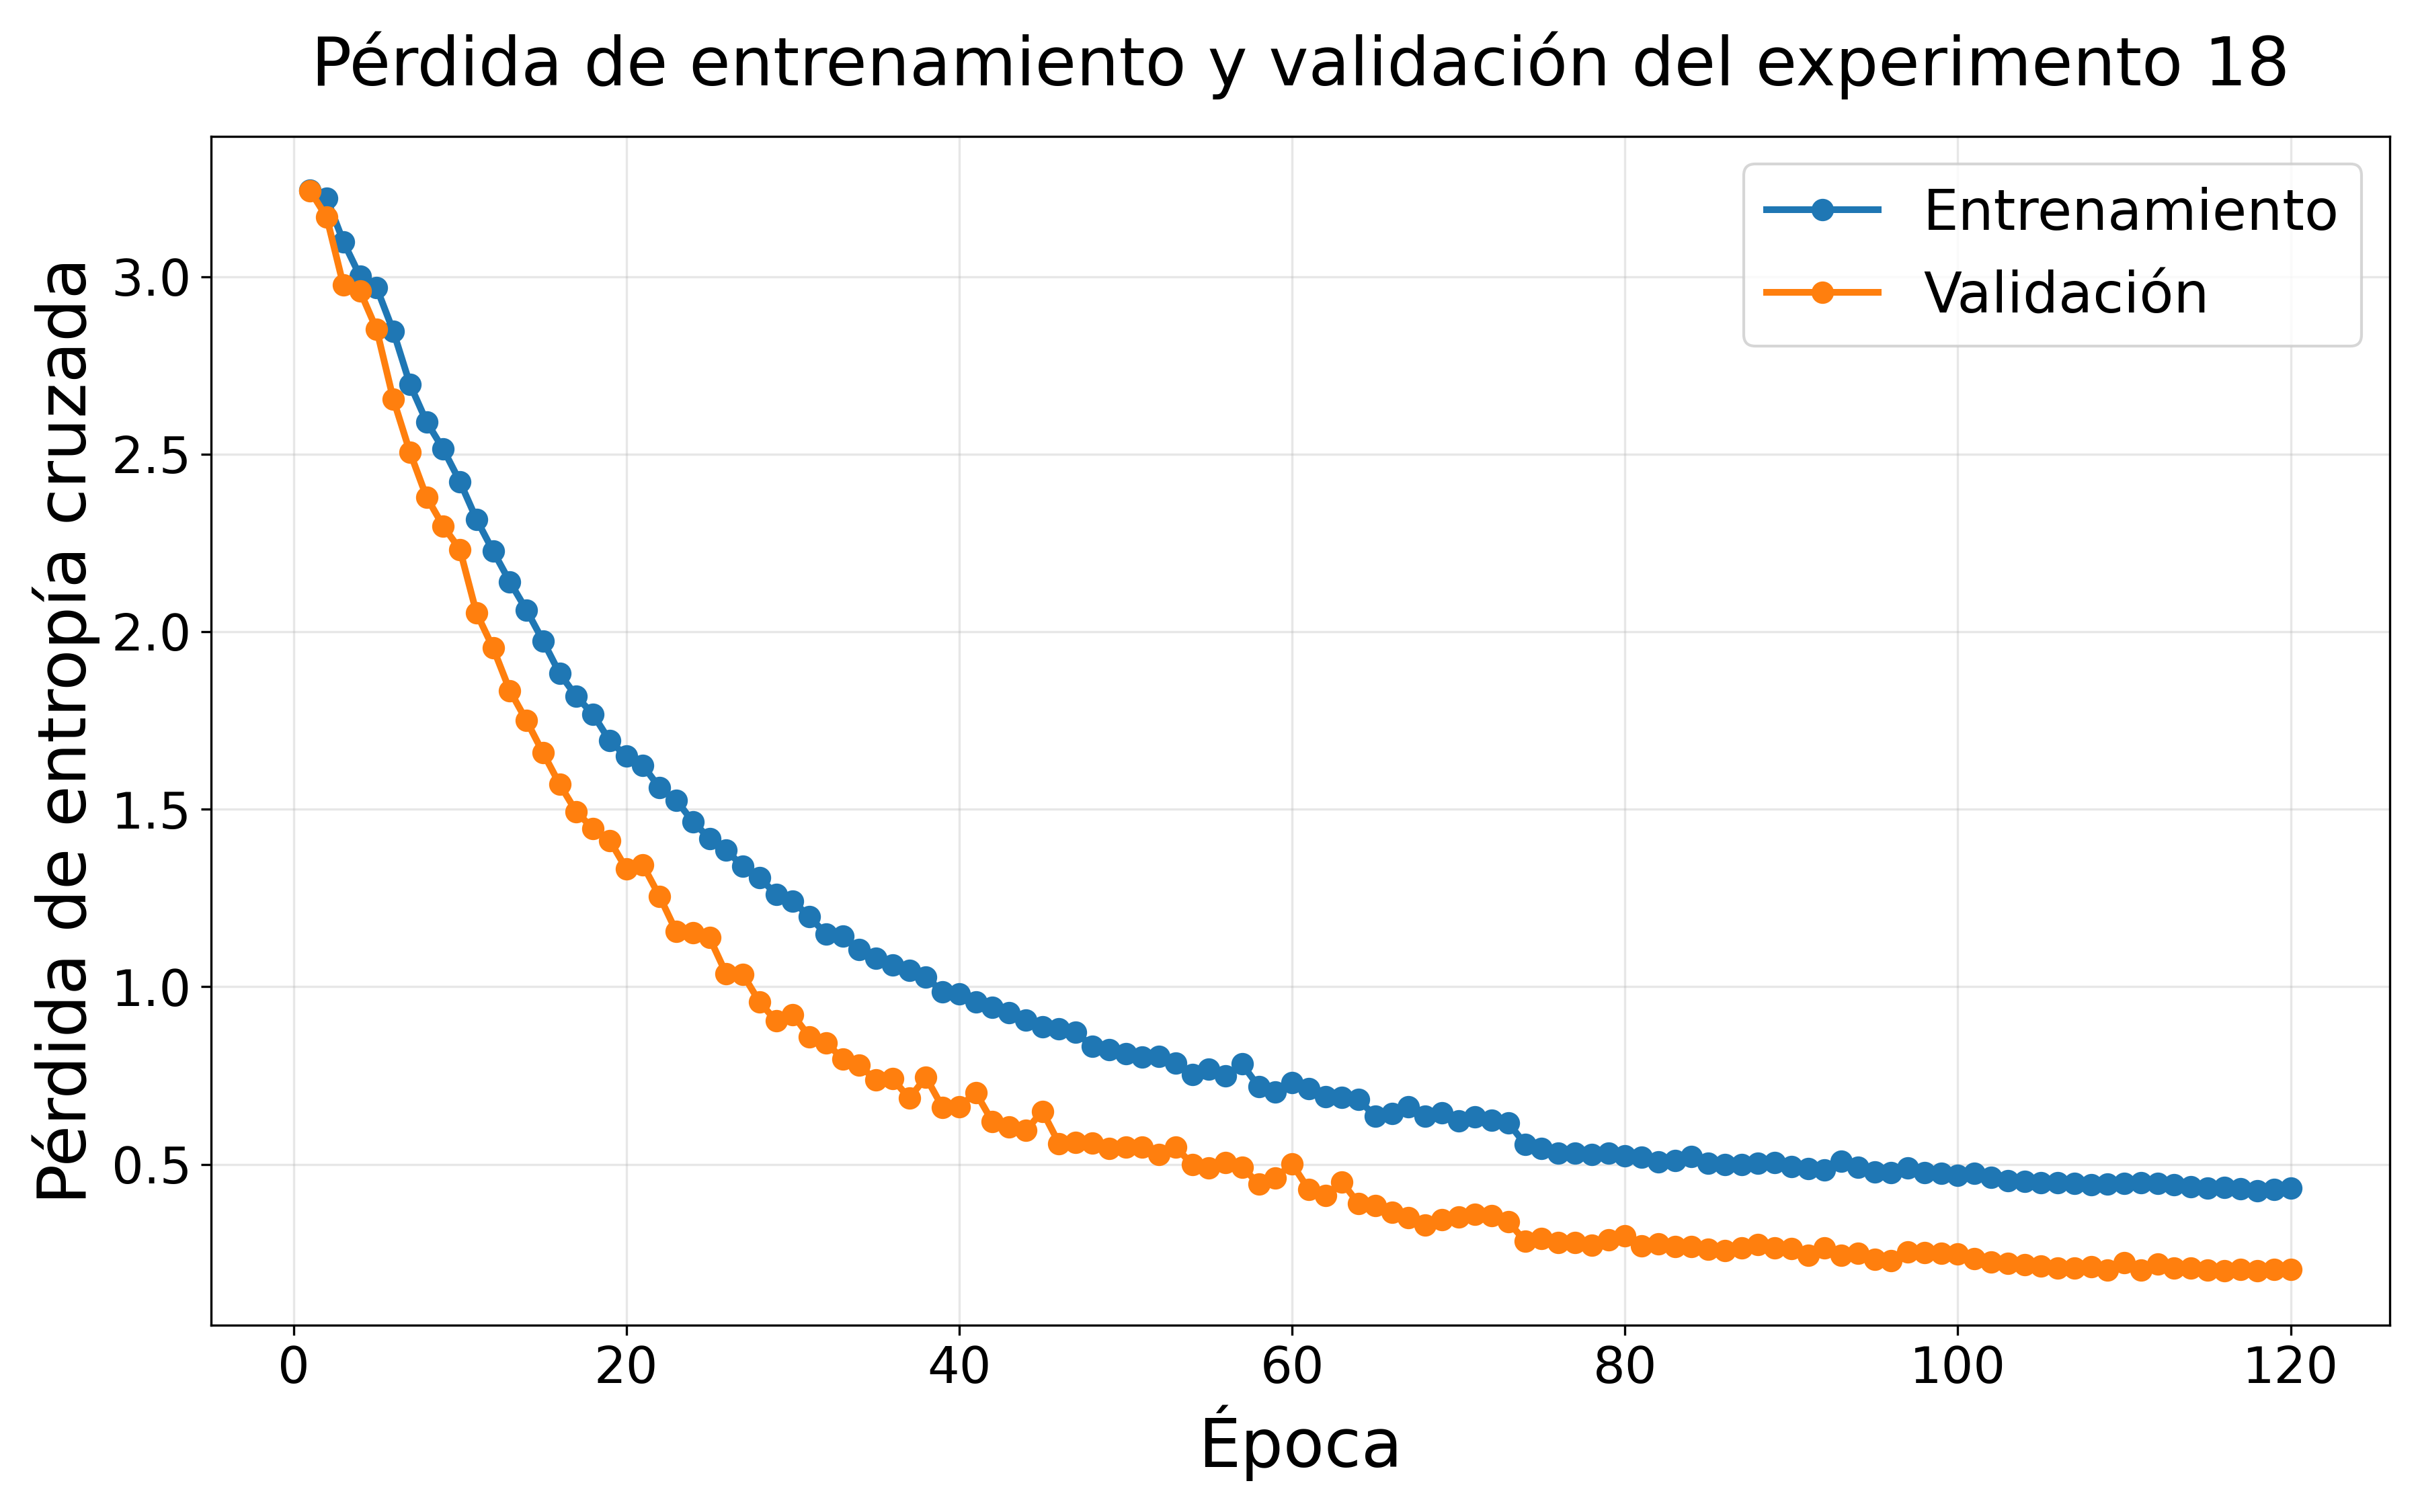
\includegraphics[width=\textwidth]{figures/Experiments_logs/loss_curve_05-14-1106.png}
        \caption{}
        \label{fig:loss_curve_05-14-1106}
    \end{subfigure}
    \hfill
    \begin{subfigure}{0.45\textwidth}
        \centering
        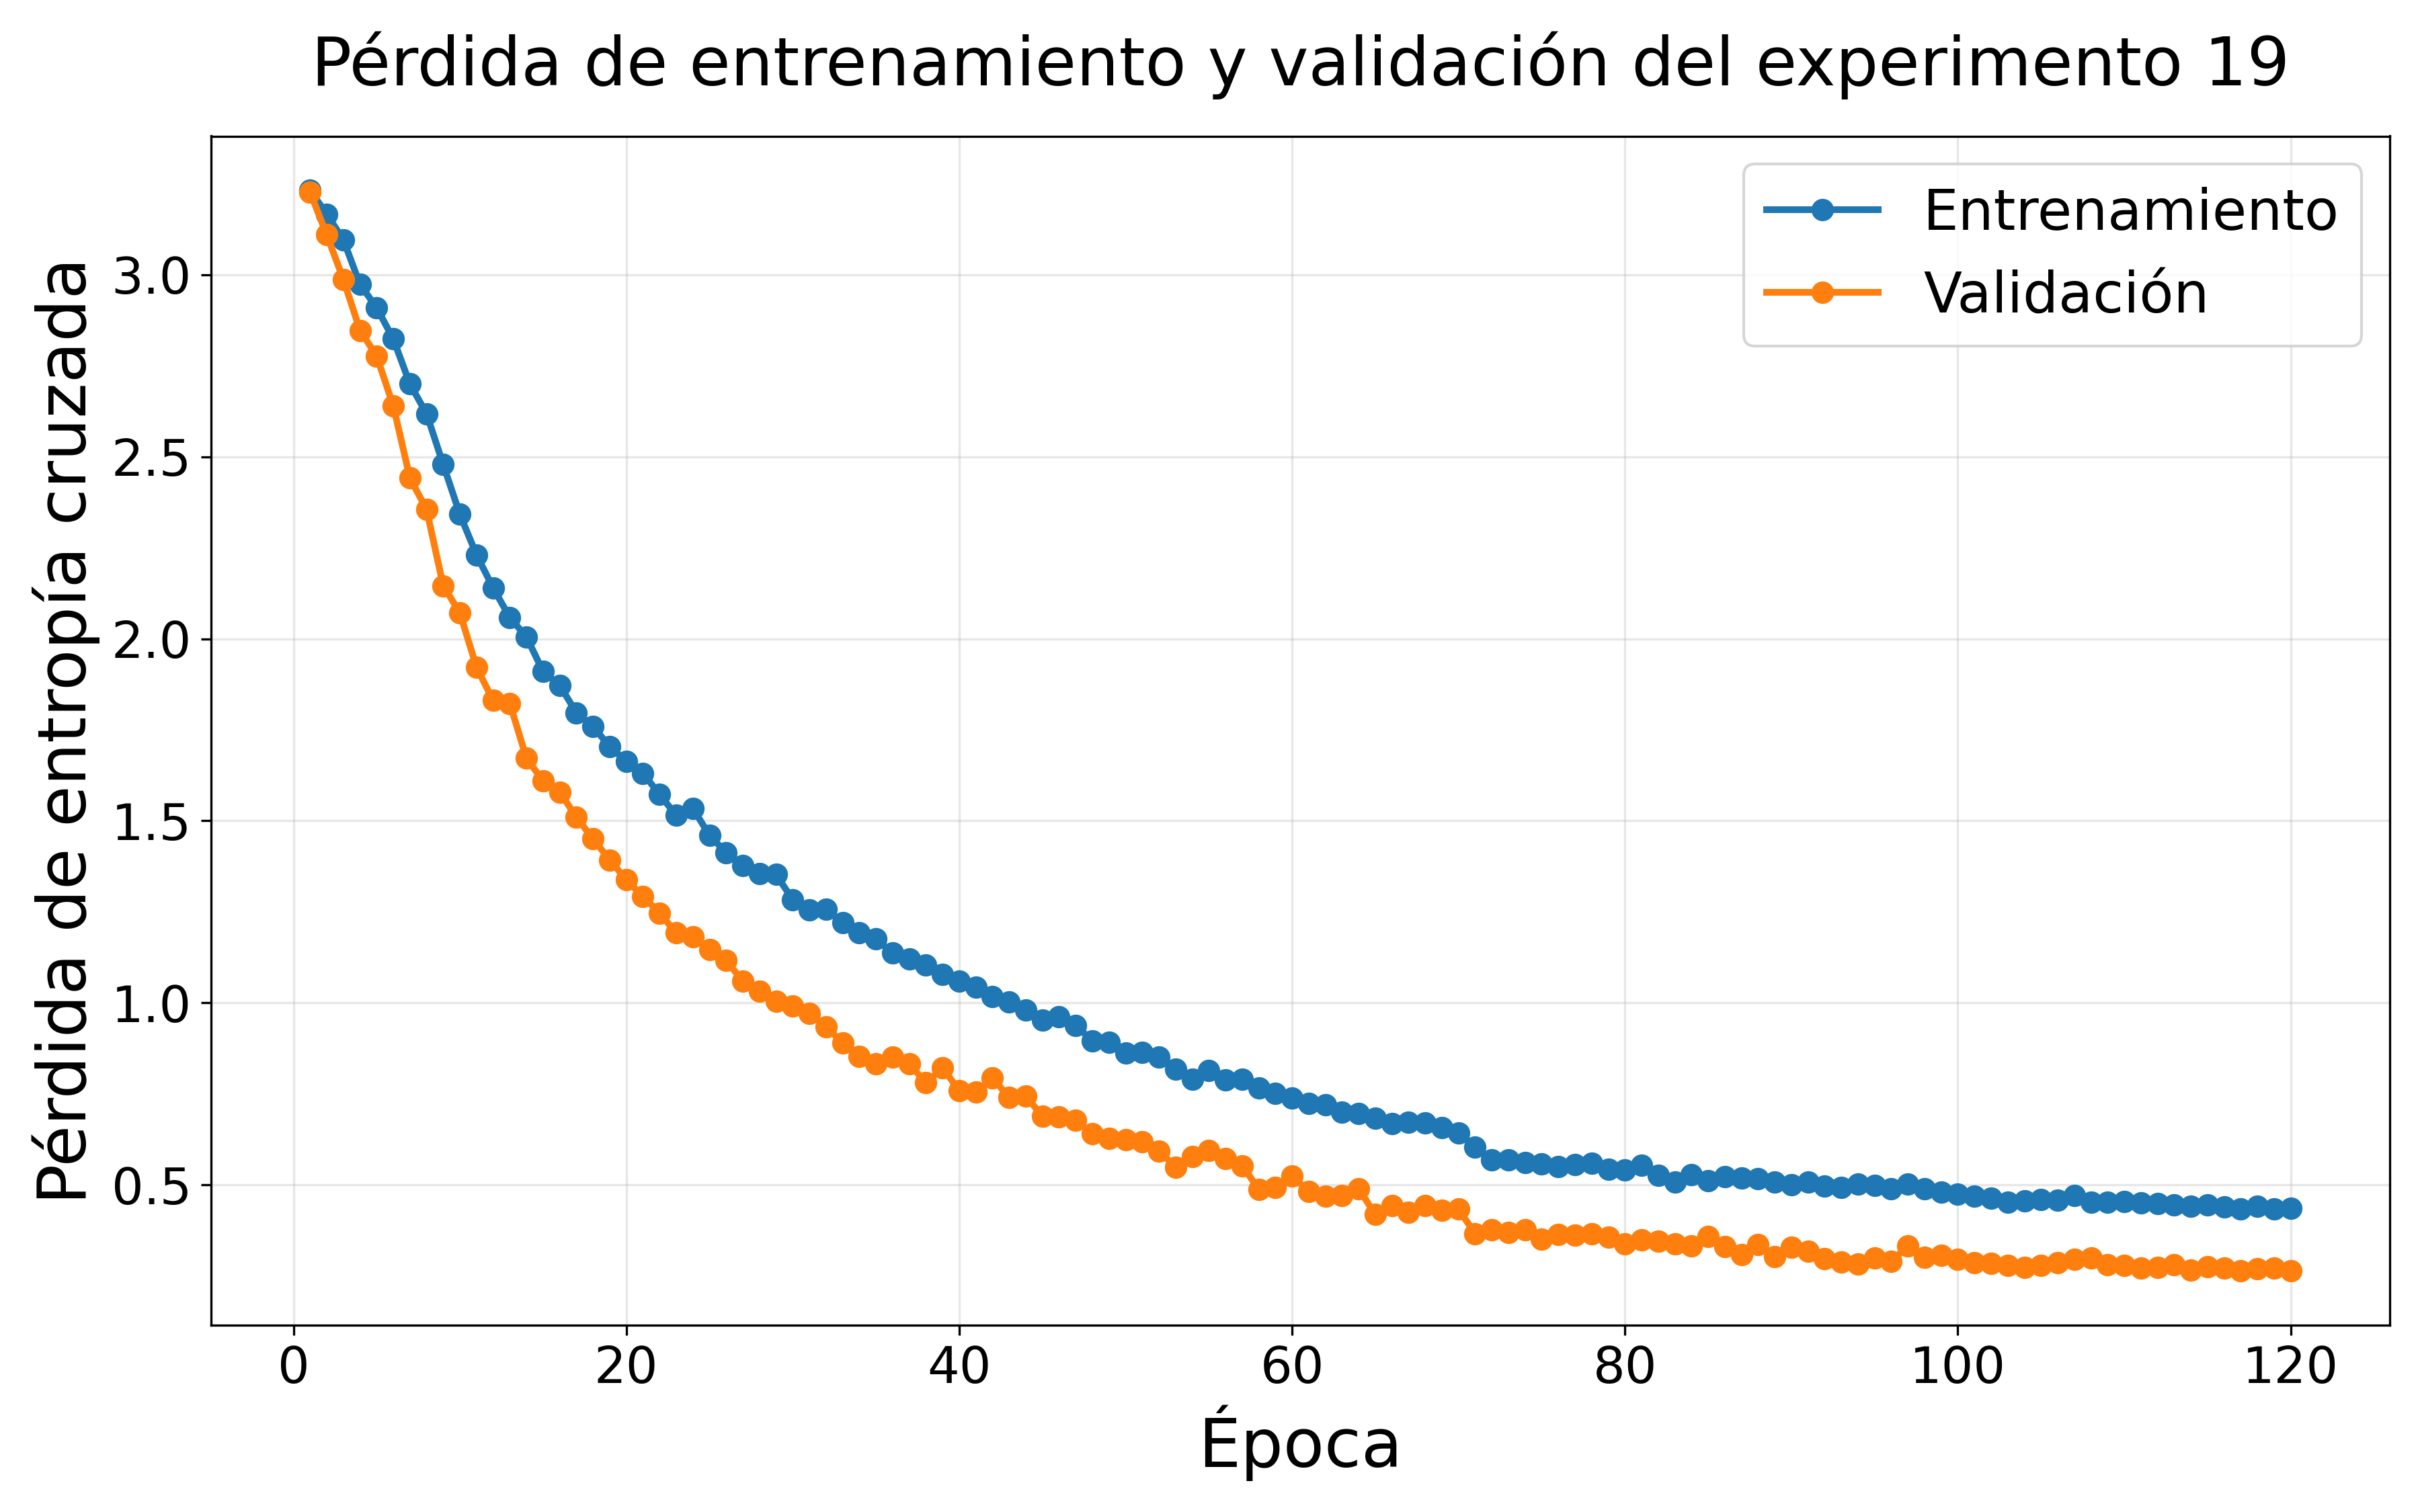
\includegraphics[width=\textwidth]{figures/Experiments_logs/loss_curve_05-14-1107.png}
        \caption{}
        \label{fig:loss_curve_05-14-1107}
    \end{subfigure}

    \caption{Experimentos realizados con el cambio del \textit{data augmentation}}
    \label{fig:loss_curve_05-14}
\end{figure}

Este fue el salto más grande del proyecto. Antes de esta modificación, el mejor resultado estaba alrededor de 88,94\%. Con \textit{data augmentation light}, los cuatro experimentos superaron el 94\%, y la mejor llegó a 96,05\%. Estos resultados confirman las hipótesis 4; la preparación de datos y la regularización visual fueron decisivas.

\section{Mejor modelo obtenido}

El experimento con mejores resultados es el número 18. La configuración principal fue la siguiente. \textit{Seed} 69, dimensión 12/12, embedding AIM, \texttt{HybridCustomTTN}, cabeza lineal, \textit{learning rate} 0,00025, warmup coseno de 5 épocas, label smoothing 0,05, regularización $L_2$ suave, preservación de relación de aspecto y aumento de datos \texttt{light}.

\begin{table}[H]
\centering
\small
\begin{tabular}{lc}
\toprule
\textbf{Métrica} & \textbf{Valor} \\
\midrule
Accuracy top-1 & 96,05\% \\
Accuracy top-5 & 99,43\% \\
Macro precision & 96,12\% \\
Macro recall & 95,82\% \\
Macro F1 & 95,94\% \\
Weighted F1 & 96,05\% \\
\texttt{classification\_mAP} & 98,41\% \\
Eval loss final & 0,2037 \\
\bottomrule
\end{tabular}
\caption{Métricas principales del mejor modelo sobre ChemEq25.}
\label{tab:mejor_modelo}
\end{table}

\begin{figure}[htbp]
    \centering

    \begin{subfigure}{0.45\textwidth}
        \centering
        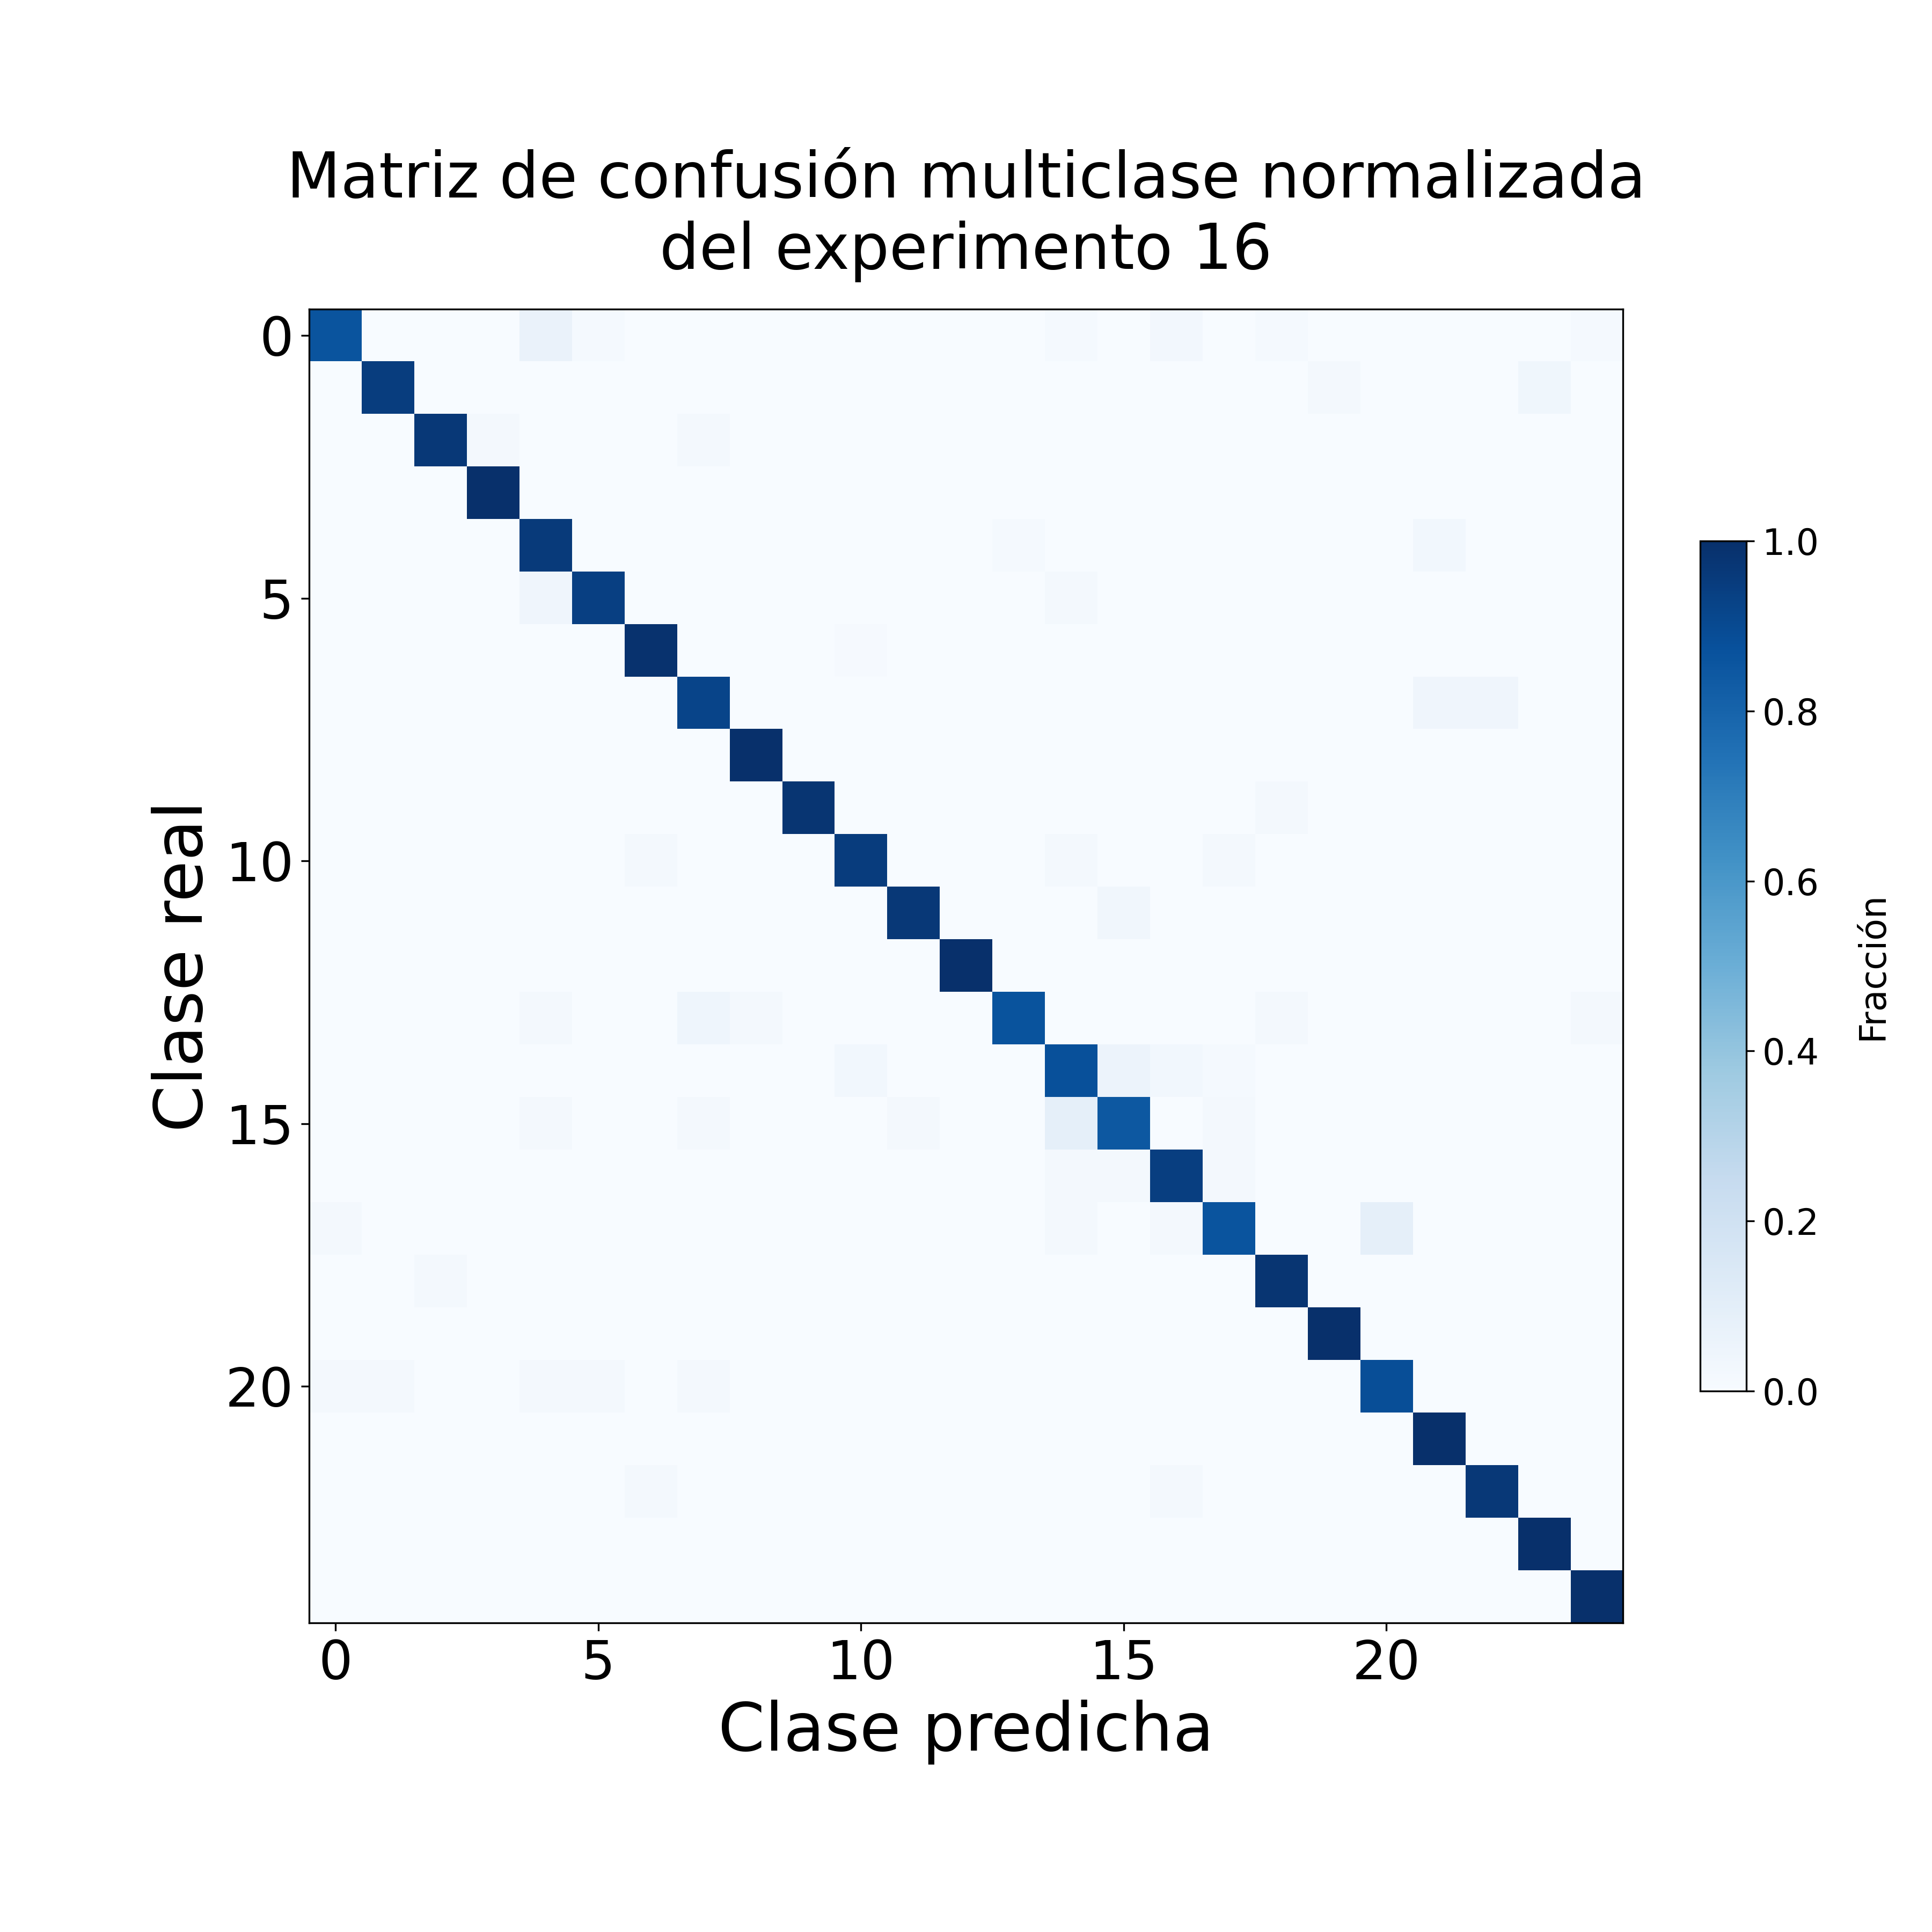
\includegraphics[width=\textwidth]{figures/Experiments_logs/confusion_matrix_05-14-1025.png}
        \caption{}
        \label{fig:confusion_matrix_05-14-1025}
    \end{subfigure}
    \hfill
    \begin{subfigure}{0.45\textwidth}
        \centering
        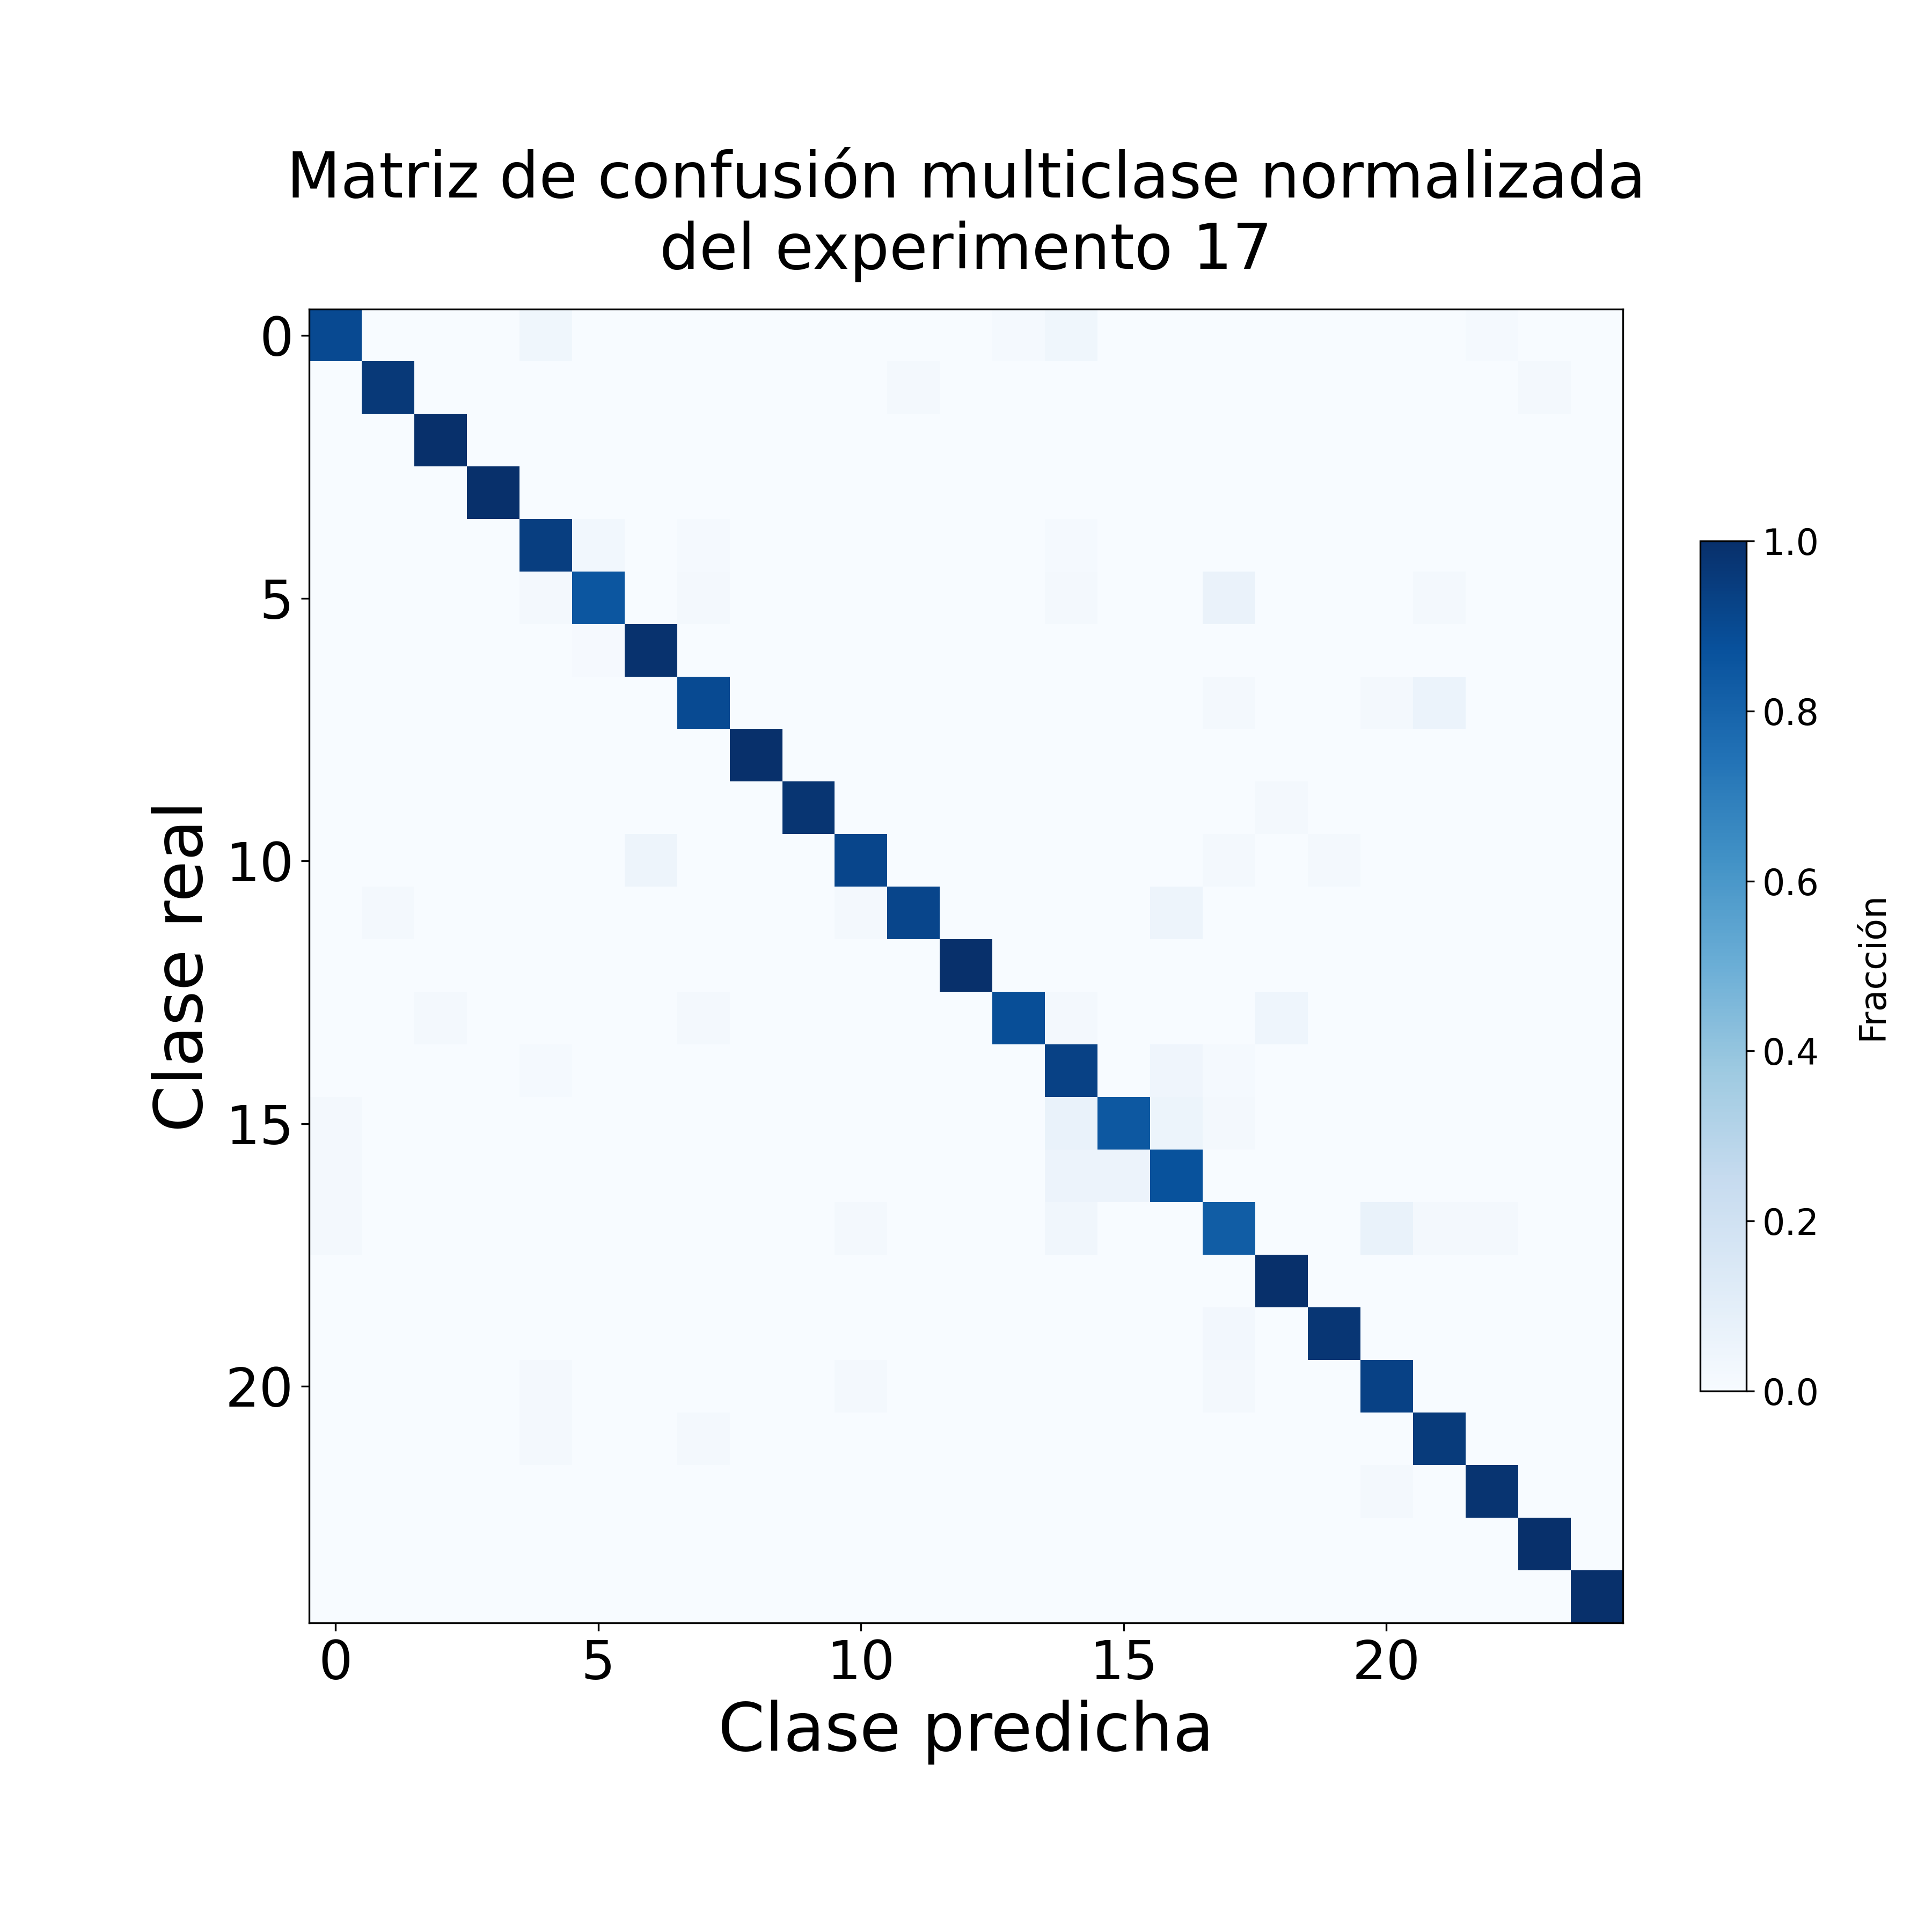
\includegraphics[width=\textwidth]{figures/Experiments_logs/confusion_matrix_05-14-1026.png}
        \caption{}
        \label{fig:confusion_matrix_05-14-1026}
    \end{subfigure}

    \vspace{0.4cm}

    \begin{subfigure}{0.45\textwidth}
        \centering
        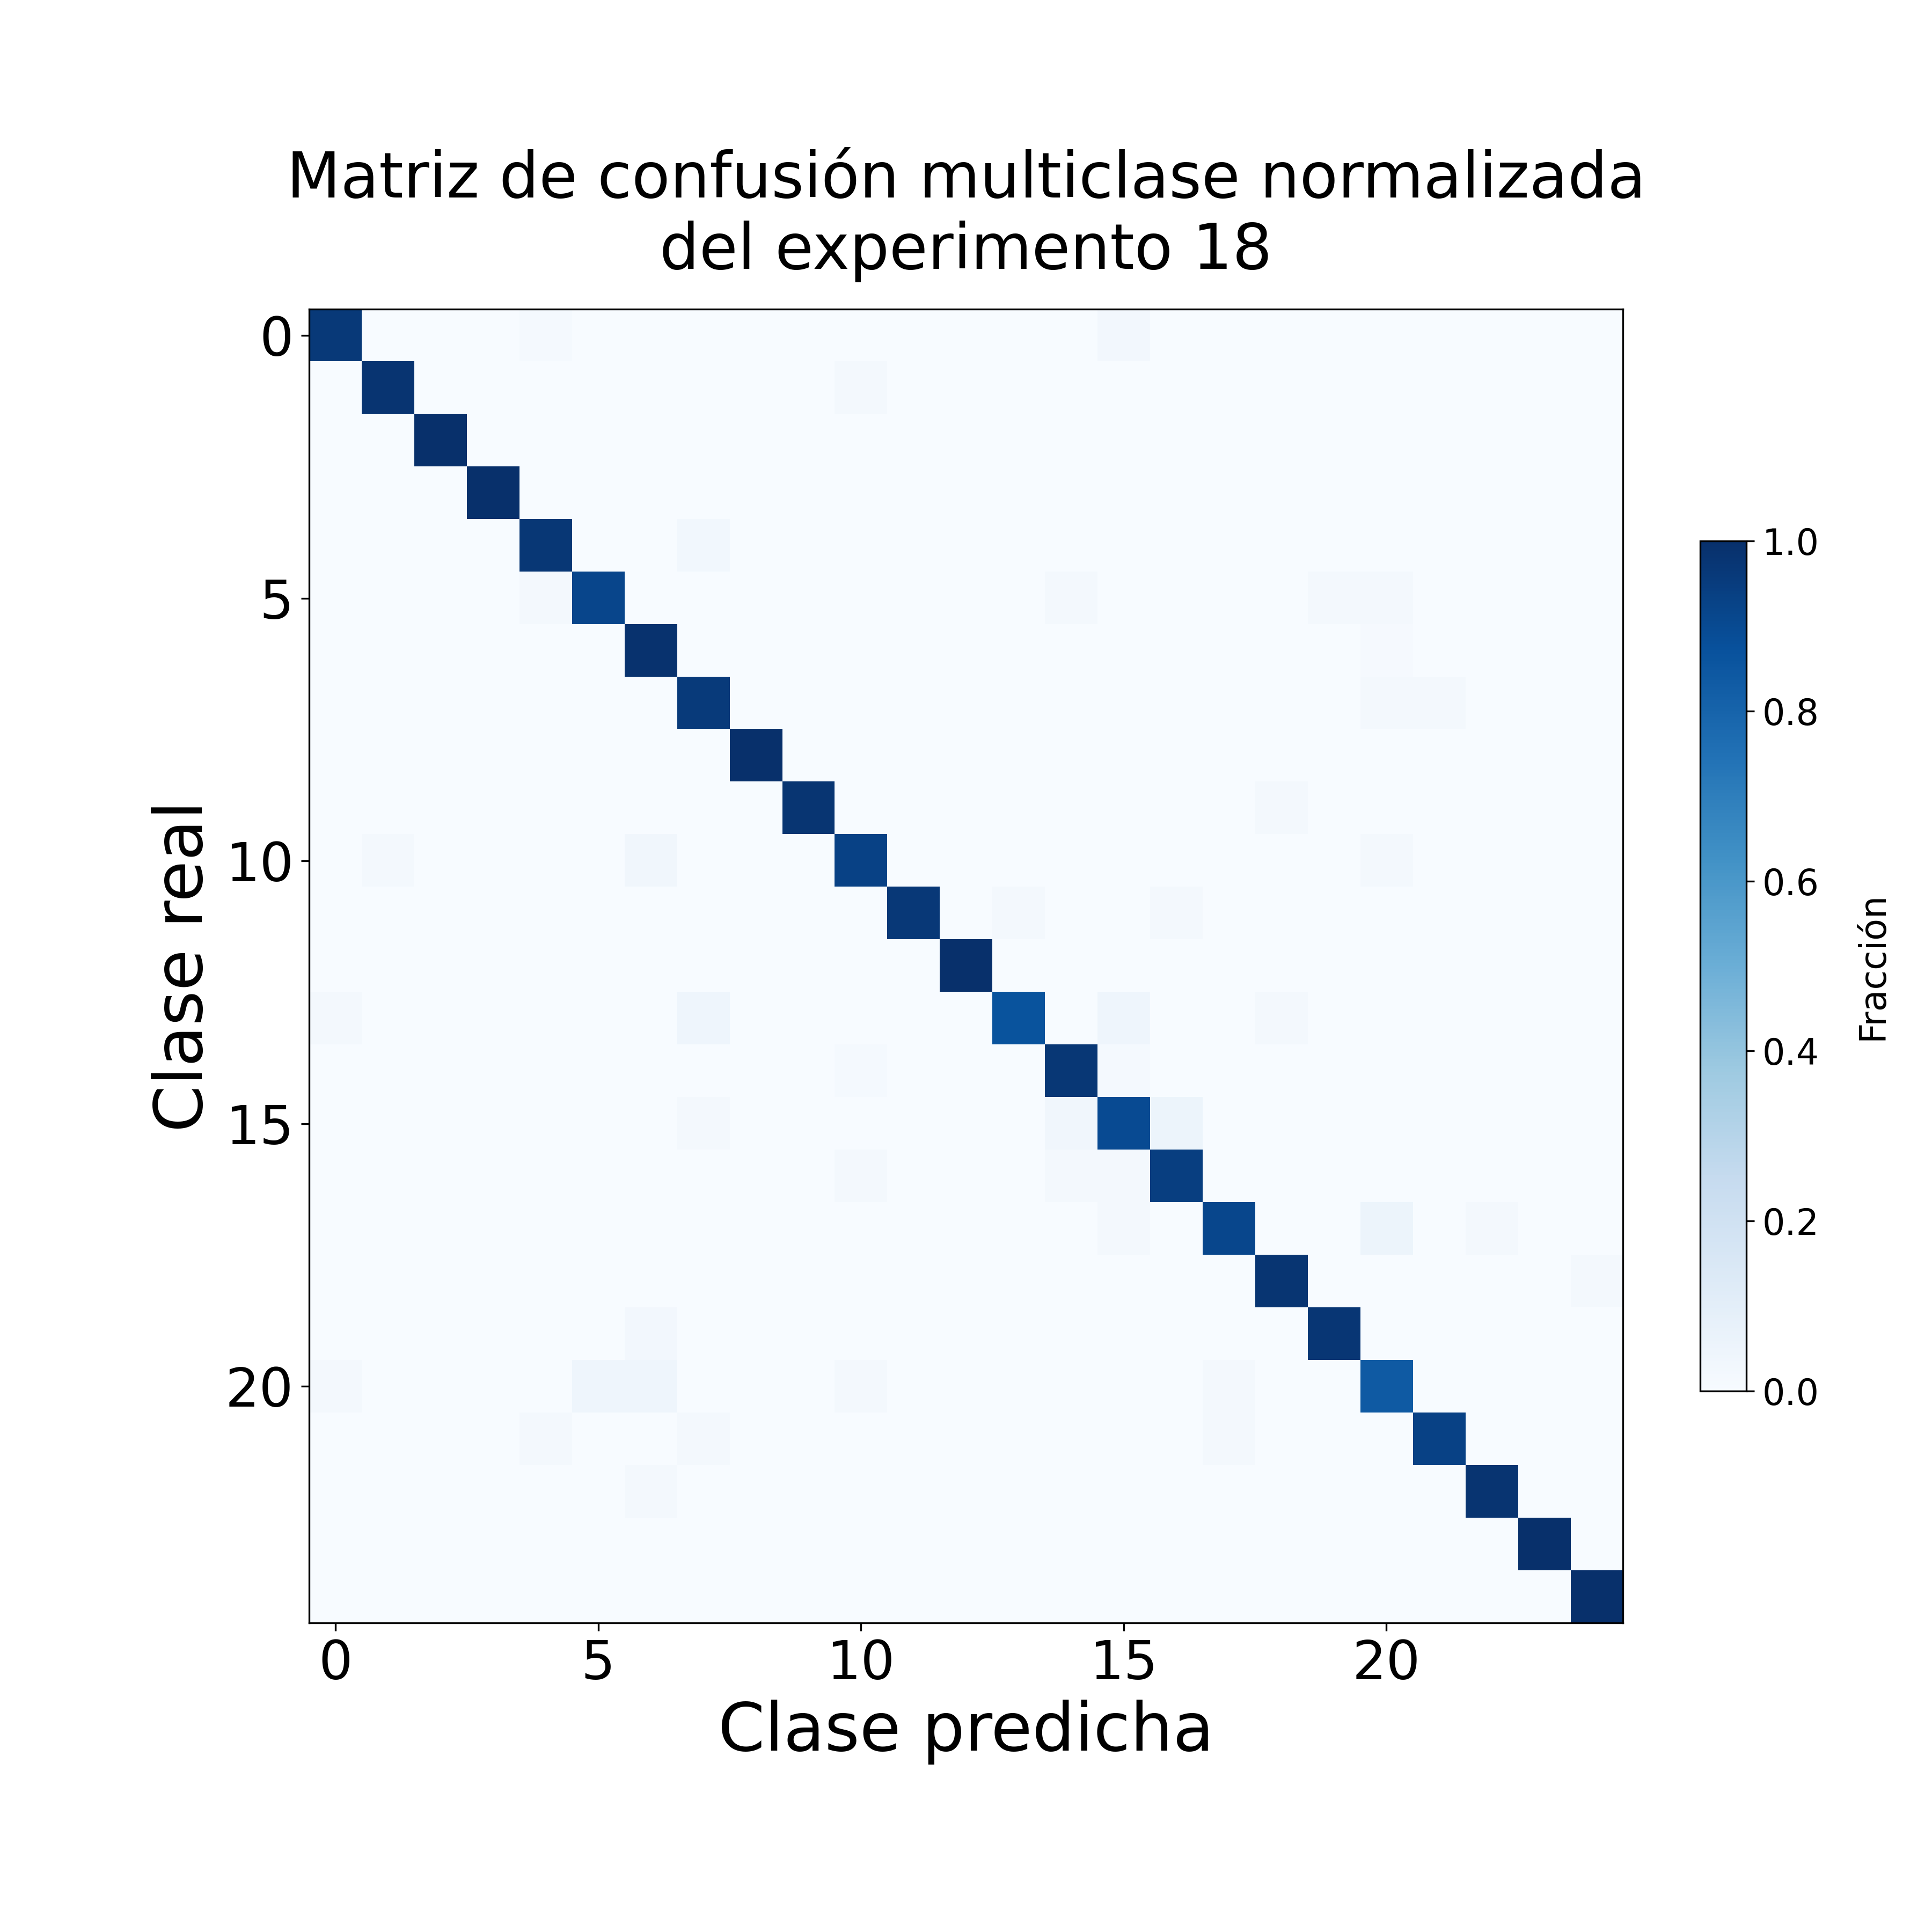
\includegraphics[width=\textwidth]{figures/Experiments_logs/confusion_matrix_05-14-1106.png}
        \caption{}
        \label{fig:confusion_matrix_05-14-1106}
    \end{subfigure}
    \hfill
    \begin{subfigure}{0.45\textwidth}
        \centering
        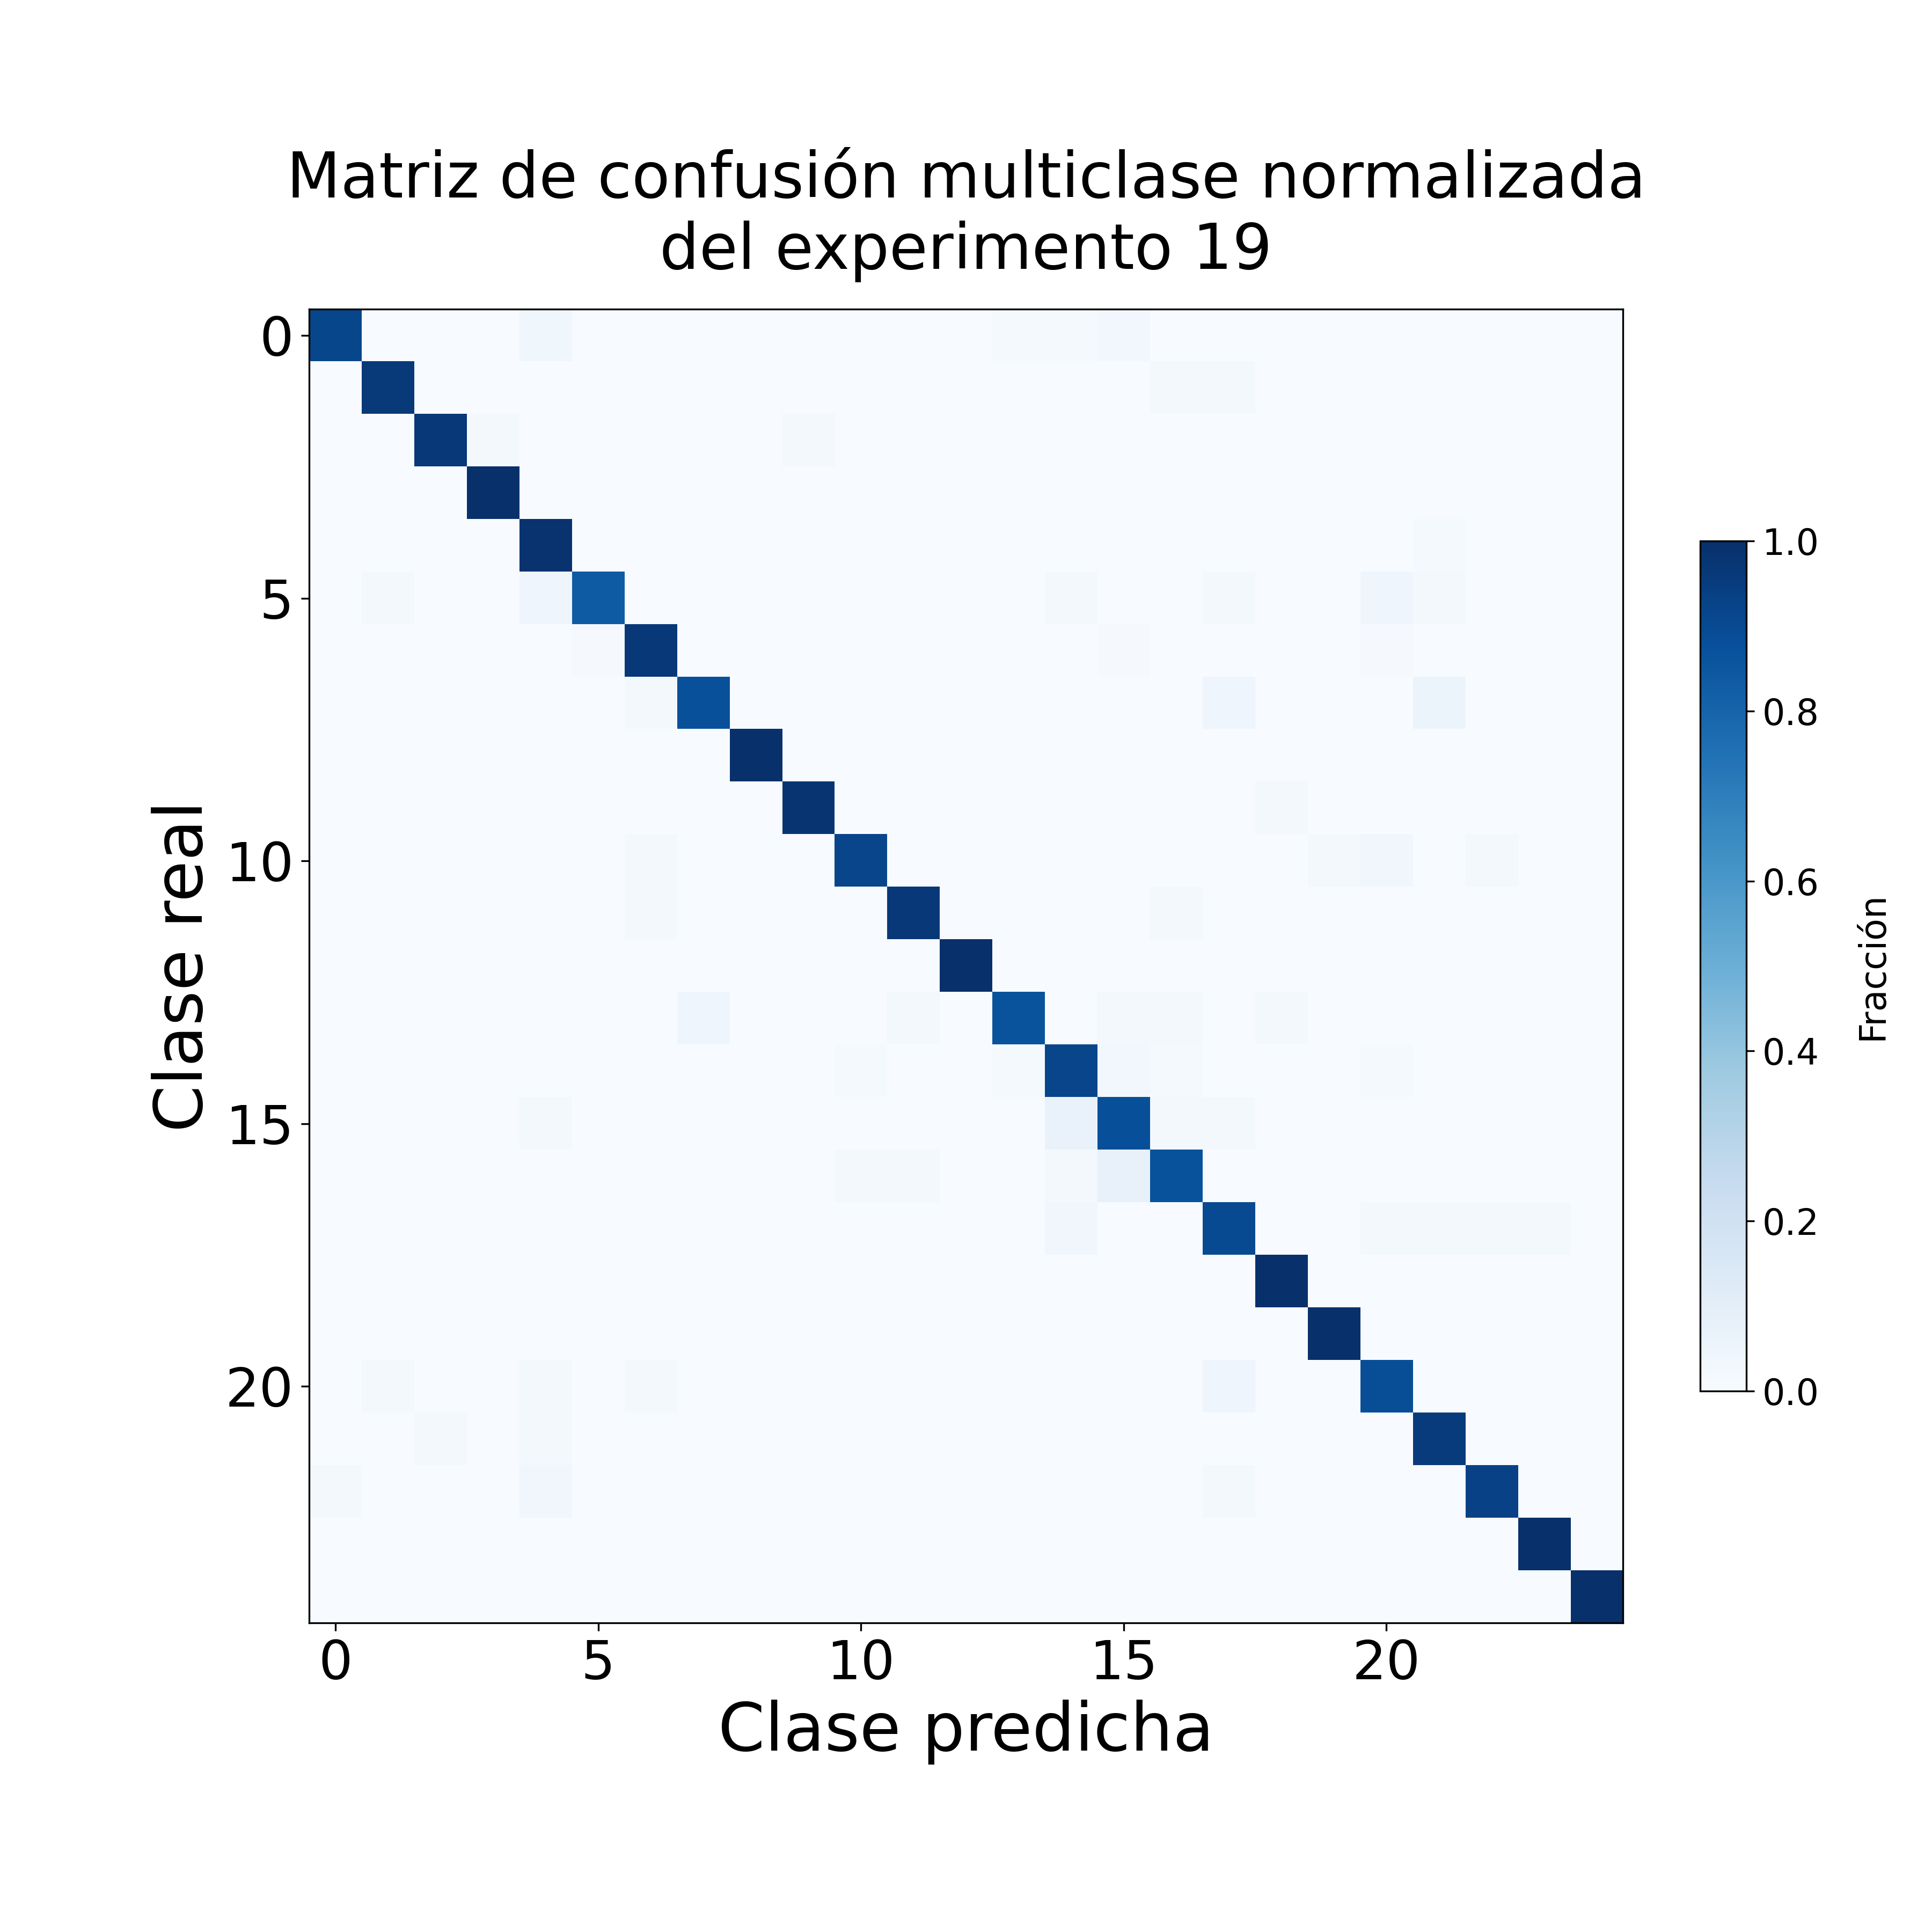
\includegraphics[width=\textwidth]{figures/Experiments_logs/confusion_matrix_05-14-1107.png}
        \caption{}
        \label{fig:confusion_matrix_05-14-1107}
    \end{subfigure}

    \caption{Matrices de confusión de los experimentos después de aplicar \textit{data augmentation}}
    \label{fig:confusion_matrix-05-14}
\end{figure}

Las matrices de confusión $\bigr($\figref{fig:confusion_matrix-05-14}$\bigl)$ muestran una diagonal muy marcada. Esto significa que el modelo clasifica correctamente la gran mayoría de los recortes. Los errores que quedan se concentran en clases visualmente parecidas. En el mejor experimento, las clases con F1 más bajo siguieron siendo algunas de las más difíciles del dataset, especialmente las relacionadas con objetos alargados o con geometría muy parecida.

El top-5 de 99,43\% también es importante. Quiere decir que, cuando el modelo no acierta la primera predicción, casi siempre tiene la clase correcta entre las cinco más probables. Esto sugiere que la representación aprendida por AIM + TTN contiene mucha información útil, aunque todavía haya confusiones finas entre clases muy similares.

La métrica \texttt{classification\_mAP} fue 98,41\%. Esta métrica se calculó como una media de precisión one-vs-rest sobre las probabilidades de clase. No debe confundirse con el \textit{mAP@50} de detección del paper de ChemEq25, porque aquí no se evalúan cajas ni IoU. Aun así, es una señal muy fuerte de que el ranking de probabilidades del clasificador es muy bueno.

\section{Variabilidad por seed y límite de las pruebas finales}

Después de alcanzar el 96,05\%, se lanzó una \textit{seed sweep} con la misma configuración para comprobar la robustez del modelo.

\begin{table}[H]
\centering
\small
\begin{tabular}{lccccc}
\toprule
\textbf{Experimento} & \textbf{Seed} & \textbf{Mejor acc.} & \textbf{Top-5} & \textbf{Macro F1} & \textbf{Acc. final} \\
\midrule
\texttt{20} & 17 & 92,96\% & 98,42\% & 92,88\% & 91,89\% \\
\texttt{21} & 88 & 93,40\% & 98,78\% & 93,41\% & 92,39\% \\
\texttt{22} & 123 & 92,25\% & 98,56\% & 92,33\% & 91,17\% \\
\texttt{23} & 314 & 93,54\% & 98,49\% & 93,57\% & 93,18\% \\
\midrule
\textbf{Media} & -- & \textbf{93,04\%} & -- & \textbf{93,05\%} & -- \\
\bottomrule
\end{tabular}
\caption{Seed sweep posterior al mejor resultado.}
\label{tab:seed_sweep}
\end{table}

Ninguno de los experimentos superó a \texttt{ChemEq\_exp15}. Todas quedaron entre 92,25\% y 93,54\%, por debajo del mejor experimento del 14 de mayo. Esto muestra que la \textit{seed} tiene un efecto fuerte.

También se probó aumentar la capacidad a \texttt{local\_dim=14} y \texttt{bond\_dim=14}, pero en esa prueba el resultado cayó a 88,16\%. Esto refuerza una idea importante: en este proyecto, más capacidad no siempre significa mejor generalización. Los cambios que más ayudaron fueron los que mejoraron la información visual y la regularización, no simplemente aumentar dimensiones.

\section{Resumen de la evolución experimental}

La evolución completa del proyecto se resume en la siguiente tabla:

\begin{table}[H]
\centering
\small
\begin{tabularx}{\textwidth}{lXc}
\toprule
\textbf{Fase} & \textbf{Cambio principal} & \textbf{Mejor accuracy} \\
\midrule
Flowers, CustomTTN inicial & TTN propia sin transformaciones intermedias & 3,58\% \\
Flowers, HybridCustomTTN & Transformaciones no lineales entre niveles & 13,60\% \\
Flowers, AIM + augmentation & Front-end AIM y aumento de datos & 33,96\% \\
ChemEq25 inicial & Cambio al dataset principal por crops & 57,00\% \\
ChemEq25 con LR menor & Optimización más estable & 75,23\% \\
ChemEq25 ajustado & Warmup, 12/12, regularización y label smoothing & 88,94\% \\
ChemEq25 final & \textit{Data augmentation light} y mejor seed & 96,05\% \\
\bottomrule
\end{tabularx}
\caption{Resumen global de la evolución experimental del proyecto.}
\label{tab:resumen_evolucion}
\end{table}

La lectura final es que el modelo basado en TN sí consiguió aprender una tarea visual real. El mejor resultado, 96,05\% de accuracy y 95,94\% de macro F1 en ChemEq25, demuestra que la arquitectura AIM + \texttt{HybridCustomTTN} es una alternativa viable para clasificación de imágenes de material de laboratorio.